\chapter{Desenvolvimento do sistema de suporte à decisão} \label{chap:desenvolvimento}  % ##   5

Este capítulo visa apresentar todo o processo realizado para o desenvolvimento do sistema de suporte à decisão. O propósito desta aplicação é auxiliar o coordenador do curso de Ciência da Computação da UENF na alocação interativa de turmas, professores e salas. O auxílio é dado através de duas formas: a primeira é a \hyperref[par:Solução inicial]{criação automatizada da grade baseada no histórico das grades anteriores}, a segunda é a \hyperref[sec:conflitos]{identificação de conflitos}, como a alocação de uma turma grande demais para a capacidade da sala, com o objetivo de auxiliar no aprimoramento da grade inicialmente gerada.

Inicia-se com a apresentação de \hyperref[sec:projetos]{projetos anteriores} que serviram de base para o desenvolvimento do presente trabalho. Em seguida, será apresentado o \hyperref[sec:LGPD]{acesso aos dados acadêmicos da instituição} e as dificuldades encontradas para a sua obtenção. Posteriormente, será apresentado o processo de \hyperref[sec:prototipagem]{prototipagem} do sistema, onde foram criados os designs iniciais das telas do sistema. Em seguida, será apresentado o processo de \hyperref[sec:programação]{programação do sistema}, que foi dividido em três grandes categorias que visavam entregar o sistema de forma gradual e funcional.

Por fim, será apresentado o cerne do sistema que é a \hyperref[sec:conflitos]{identificação e visualização de conflitos}, ou seja, os casos em que a alocação dos recursos gera algum comportamento minimamente indesejável como por exemplo a alocação de uma sala a duas turmas ao mesmo tempo. Serão apresentados os tipos de conflitos que o sistema é capaz de identificar, como eles são visualizados e como o sistema lida com cada um deles. Conclui-se então com a apresentação do \hyperref[sec:preenchimento]{preenchimento do banco de dados} com dados reais.

\section{Projetos anteriores} \label{sec:projetos}                                      % ###  5.1

Antes do desenvolvimento do presente trabalho, outros projetos já foram idealizados e até mesmo desenvolvidos. Dentre eles, dois se destacam por terem sido os precursores do atual projeto. O primeiro deles, que foi idealizado, mas não desenvolvido, almejava apresentar uma \hyperref[ssec:andamento]{visualização da progressão dos alunos na grade curricular}. O segundo, que foi desenvolvido, realizava o \hyperref[ssec:demanda]{cálculo da demanda}, ou seja, calculava quantos e quais eram os alunos que poderiam se inscrever nas disciplinas. Ambos os projetos se mostram como abordagens paralelas de auxiliar no planejamento do curso de Ciência da Computação da UENF, sendo eles também sistemas de suporte à decisão, mesmo que em menor escala.

Deve-se comentar também sobre os dois trabalhos anteriores desenvolvidos por \citeonline{SanyaSantos2013} e \citeonline{RicardoSilveira2014} que iniciaram os estudos sobre a alocação de turmas no curso de Ciência da Computação na UENF, que foram \hyperref[sec:anteriores]{citados previamente}.

\subsection{Andamento dos alunos} \label{ssec:andamento}                                % #### 5.1.1

% Como interesse próprio, c
Cogitou-se o desenvolvimento de uma plataforma onde se pudesse ver em que ponto os alunos se encontram em relação à grade curricular de seus cursos. Para isso, seria necessária a obtenção dos dados dos alunos, seja por parte dos mesmos, do coordenador ou por integração com o sistema acadêmico. Com estes dados, seria possível criar uma interface que mostrasse o andamento dos alunos, quais matérias já foram cursadas, quais estão sendo cursadas e quais ainda faltam. Além disso, seria possível mostrar quais matérias são pré-requisitos para outras. Assim, o aluno e a coordenação poderiam ter uma visão geral de seu andamento e de quais matérias ele precisará cursar para se formar.
% Esse projeto não saiu do mundo das ideias, entretanto, lá permaneceu sendo maturado.

\begin{MyCenteredFigure} \caption{Andamento do aluno no Sistema Acadêmico} \label{fig:andamento}
  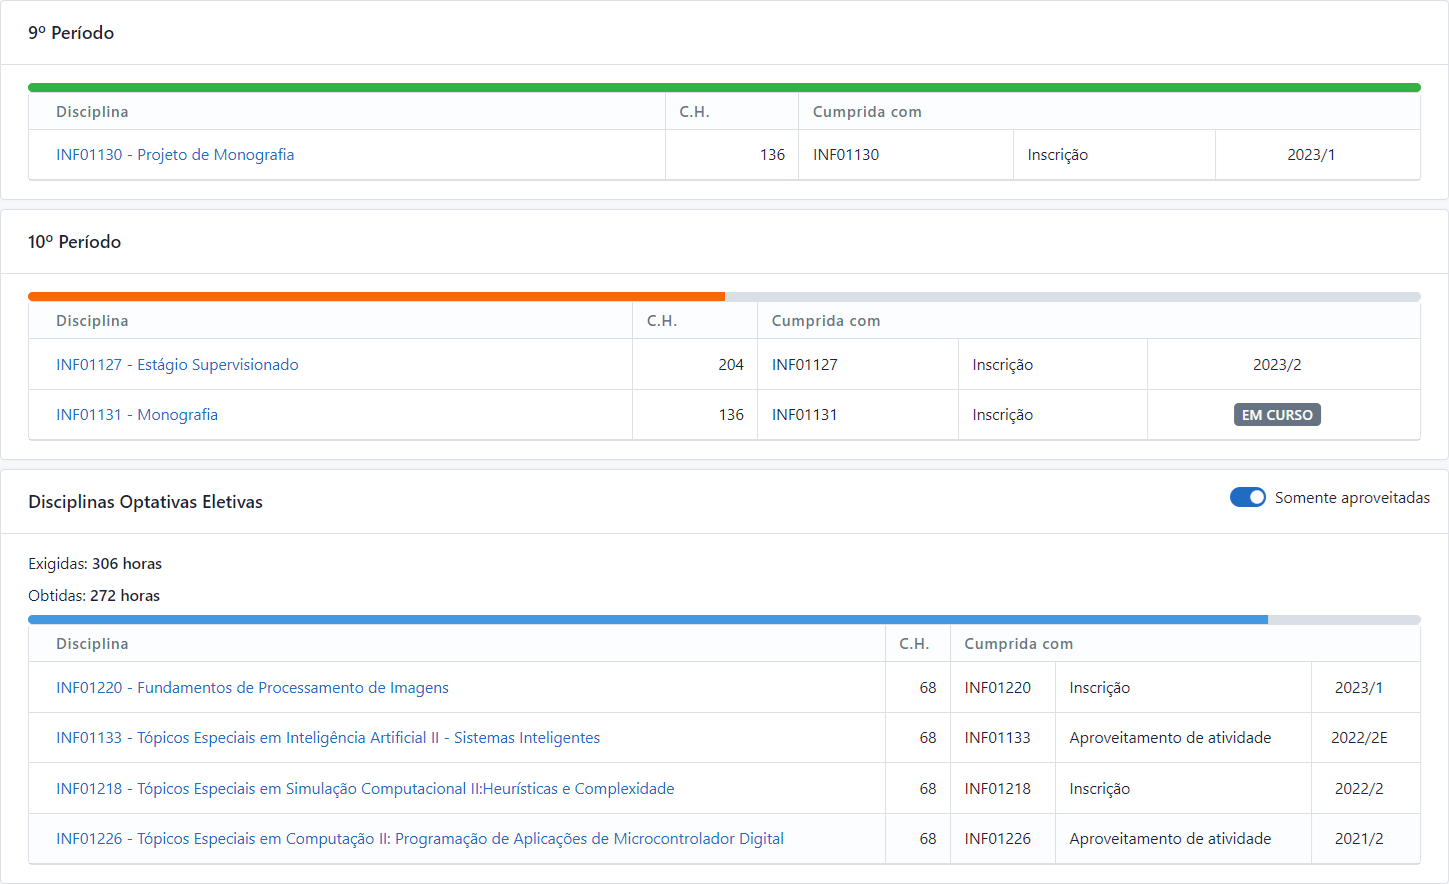
\includegraphics[width=\textwidth]{files/img/2.02!5-desenvolvimento/2.02!5.1-anteriores/Progressão}
\end{MyCenteredFigure}

Anos após a concepção dessa funcionalidade, o Sistema Acadêmico da UENF passou a disponibilizar uma funcionalidade semelhante, como pode ser visto na \autoref{fig:andamento}. Nela, é possível ver o andamento do aluno por período, incluindo as disciplinas Eletivas Livres e Eletivas Optativas. Entretanto, essa visualização tabular não ilustra o andamento de todos os alunos simultaneamente, sendo necessário navegar individualmente por cada um deles.

\subsection{Cálculo de demanda} \label{ssec:demanda}                                    % #### 5.1.2

Durante o intervalo entre os semestres, os alunos precisam se inscrever nas matérias que desejam cursar no semestre seguinte. Para isso, é necessário que o coordenador saiba quantos alunos estão interessados em cada matéria para que ele possa definir quantas turmas serão abertas. Com este fim em mente, o coordenador dispõe de algumas alternativas como estimar quantos alunos se inscreverão em cada disciplina, checar manualmente no sistema acadêmico quais alunos podem fazer cada matéria, ou então obter diretamente dos alunos através de um formulário em quais disciplinas cada um dos alunos tem a intenção de cursar.

O método que o atual Coordenador de Ciência da Computação utiliza consiste em baixar o extrato de todos os alunos do curso e tabelar no Excel qual é o andamento de cada um dos alunos, para que assim, através da análise manual, pudesse ver qual é o andamento de cada um e quantos alunos demandam quais disciplinas.

Entretanto, todas essas alternativas são trabalhosas e propensas a erros. Sendo assim, foi pensado em uma forma de automatizar esse processo. Foi então elaborado um código em \LinkToURL{\LinkPython}{Python} que atualmente \LinkToURL{\LinkProjetoDemanda}{se encontra no GitHub}. Este código tem como entrada os extratos de matrícula dos alunos e como saída a listagem das disciplinas demandadas e a listagem dos alunos que demandam cada disciplina.

\lstinputlisting[language={Python}, captionpos={t}, label={code:demand}, caption={Obter demanda por extratos em PDF}]{files/codigos/demanda.py}

Este código foi desenvolvido em 8 etapas, vistas no \autoref{code:demand}, cada uma com um arquivo separado. Para alcançar a lista das demandas, é necessário primeiro obter a lista dos arquivos em formato PDF que serão processados, em seguida extrair seus dados com a biblioteca \LinkToURL{\LinkPDFMiner}{\textit{PDFMiner}}, estruturar os dados obtidos, filtrar os dados estruturados, obter a demanda de cada disciplina, juntar as demandas de cada disciplina e salvar os dados obtidos em um arquivo de texto.

Embora o código cumpra com seu objetivo, apresenta algumas características limitantes. A primeira é que os PDFs precisam ser obtidos manualmente, um por um, pelo coordenador, sendo ela por si só uma tarefa extenuante, o que não é desejado. Além disso, o seu uso não é muito intuitivo, sendo necessário que o usuário lide com o prompt de comando e instale as dependências necessárias, o que acaba trazendo uma dificuldade a mais ao usuário. O código também apresenta limitações por sistema operacional, não sendo garantido o seu funcionamento em sistemas operacionais diferentes do Windows.

\section{Acesso aos dados acadêmicos da instituição} \label{sec:LGPD}                   % ###  5.2

Em sua concepção original, o presente trabalho visaria integrar o sistema desenvolvido com o atual sistema acadêmico da UENF. Essa abordagem foi descartada devido às dificuldades encontradas por parte do setor administrativo da UENF que, devido à \LinkToURL{\LinkLGPD}{Lei Geral de Proteção dos Dados (LGPD)}, não podem divulgar dados dos alunos, mesmo anonimizados.

Para confirmação das informações recebidas, a LGPD foi estudada e cogitou-se que o presente estudo pudesse estar amparado pela alínea b do inciso 2º do artigo 4º do capítulo 1 da Lei Nº 13.709, de 14 de agosto de 2018. Informando este que esta lei, a LGPD, não se aplica ao tratamento de dados pessoais realizado para fins exclusivamente acadêmicos. Segundo o \LinkToURL{\LinkLGPDEstudoTécnico}{Estudo Técnico sobre o tratamento de dados pessoais para fins acadêmicos}, é reforçado que ``o tratamento de dados pessoais para fins acadêmicos deve ser sempre lícito''.

Apesar das possibilidades de meios legalmente válidos para a aquisição dos dados, optou-se por abandonar a integração com o Sistema Acadêmico e o uso de dados reais dos alunos já existentes na plataforma. Rumando-se então para uma abordagem de inserção manual de dados por parte dos usuários do sistema.

\section{Prototipagem} \label{sec:prototipagem}                                         % ###  5.3

A criação de protótipos, seguindo a abordagem tomada por \citeonline{Andre2018}, se mostra como essencial para que se mantenha a constante satisfação por parte dos \textit{stakeholders}. Isso se dá com o intuito de saber quais mudanças eles sugerem ao desenvolvimento do projeto, assim reduzindo a necessidade de retrabalho e de não alcançar as expectativas do projeto. Para este fim, foram feitos os designs iniciais das telas do sistema usando o software de design \LinkToURL{\LinkFigma}{Figma}, designs esses que representam apenas o esboço, e não um sistema funcional. Esse esboço serviu como uma base visual de como o sistema estaria no final.

\subsection{Protótipos de componentes} \label{ssec:componentes}                         % #### 5.3.1

Antes de seguir com a descrição das telas, é válido descrever os componentes que foram utilizados na construção dos protótipos. Os componentes principais são os cartões de turma (\autoref{fig:cartão_de_turma}) e as caixas de seleção (\autoref{fig:selects}).

A \autoref{fig:cartão_de_turma} mostra os cartões de turma que foram utilizados para representar as turmas criadas. O objetivo desses cartões é de apresentar de forma compacta o máximo possível de informações relevantes ao usuário. Considerando o caráter iterativo do desenvolvimento, foram criados diversas versões dos cartões, todos eles visando a apresentação de informações de forma clara, objetiva e intuitiva por parte do usuário.

Essas informações relevantes são as informações relacionadas à identificação da disciplina, do professor e da sala. Além dessas, são apresentadas informações adicionais como a quantidade de alunos que podem se inscrever na disciplina e alertas de possíveis conflitos. Em todas as versões dos cartões de turma, o código da disciplina está no canto superior esquerdo. No canto inferior direito está a quantidade de alunos que podem se inscrever na disciplina e, à sua esquerda, aqueles alunos que apresentam algum tipo de impedimento, como por exemplo ter alguma outra turma que ele possa se inscrever no mesmo horário.

\begin{MyCenteredFigure} \caption{Protótipos de cartões de turma} \label{fig:cartão_de_turma}
  \begin{subfigure}[b]{0.45\textwidth} \centering
    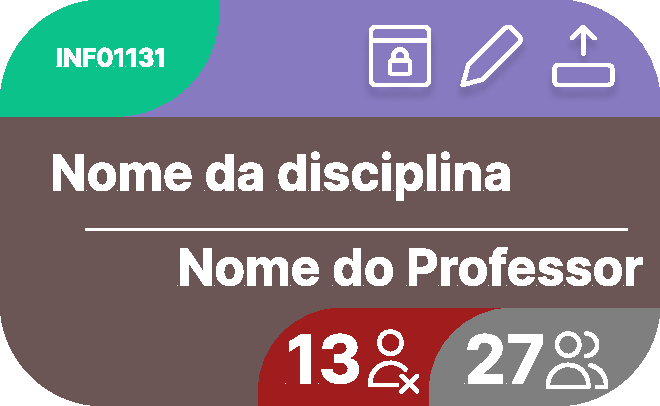
\includegraphics[width=\textwidth]{files/img/2.02!5-desenvolvimento/2.02!5.3-prototipagem/5.3.1-componentes/Cartões/PadraoClassCards}
    \caption{Turma padrão} \label{fig:TurmaPadrão}
  \end{subfigure}
  \hfill
  \begin{subfigure}[b]{0.45\textwidth} \centering
    
\includegraphics[width=\textwidth]{files/img/2.02!5-desenvolvimento/2.02!5.3-prototipagem/5.3.1-componentes/Cartões/Professor SuperiorClassCards}
    \caption{Turma com professor no topo} \label{fig:TurmaTopo}
  \end{subfigure}

  \begin{subfigure}[b]{0.45\textwidth} \centering
    
\includegraphics[width=\textwidth]{files/img/2.02!5-desenvolvimento/2.02!5.3-prototipagem/5.3.1-componentes/Cartões/Smaller ColapsadaClassCards}
    \caption{Turma colapsadas} \label{fig:TurmaColapsada}
  \end{subfigure}
  \hfill
  \begin{subfigure}[b]{0.45\textwidth} \centering
    
\includegraphics[width=\textwidth]{files/img/2.02!5-desenvolvimento/2.02!5.3-prototipagem/5.3.1-componentes/Cartões/SmallestClassCards}
    \caption{Turma com tamanho reduzido} \label{fig:TurmaColapsadaReduzida}
  \end{subfigure}
\end{MyCenteredFigure}

Nestes cartões, estão presentes também três botões: \textbf{travar}, \textbf{editar} e \textbf{expandir}/\textbf{recolher}. O botão de \textbf{travar} tem como função fixar a turma no horário em que ela se encontra, impedindo que ela seja movida. O botão de \textbf{editar} tem como função abrir um painel onde é possível alterar as informações da turma. O botão de \textbf{expandir}/\textbf{recolher} tem como função expandir ou recolher o cartão, mostrando ou escondendo informações adicionais. Em cada uma das versões dos cartões, a posição dos botões foram alteradas.

Outras informaçõe que também tiveram sua posição alterada foram o nome do professor, o nome da disciplina e o código da sala.

Cada uma dessas versões dos cartões de turma se mostra com um propósito específico. O cartão padrão (\autoref{fig:TurmaPadrão}) é um dos maiores cartões, o que facilita a visualização do usuário às informações importantes, o mesmo pode ser dito para o cartão com o professor no topo (\autoref{fig:TurmaTopo}), esse, por sua vez, distribui a posição dos botões. Já os botões colapsados (\autoref{fig:TurmaColapsada}) e o cartão com tamanho reduzido (\autoref{fig:TurmaColapsadaReduzida}) prezam por uma maior economia de espaço, sendo úteis para quando o usuário deseja visualizar mais turmas ao mesmo tempo, como é o caso da visualização da grade horária, e por isso informam também o código da sala em que estão alocados.

\begin{MyCenteredFigure} \caption{Protótipos de caixas de seleção} \label{fig:selects}
  \begin{subfigure}[b]{0.45\textwidth} \centering
    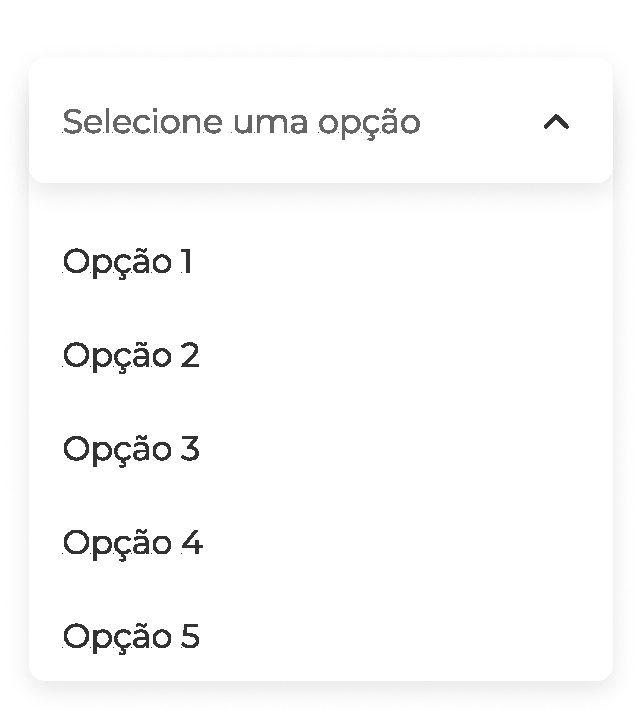
\includegraphics[width=0.8\textwidth]{files/img/2.02!5-desenvolvimento/2.02!5.3-prototipagem/5.3.1-componentes/SingleSelect}
    \caption{Caixa de seleção única} \label{fig:SingleSelect}
  \end{subfigure}
  \hfill
  \begin{subfigure}[b]{0.45\textwidth} \centering
    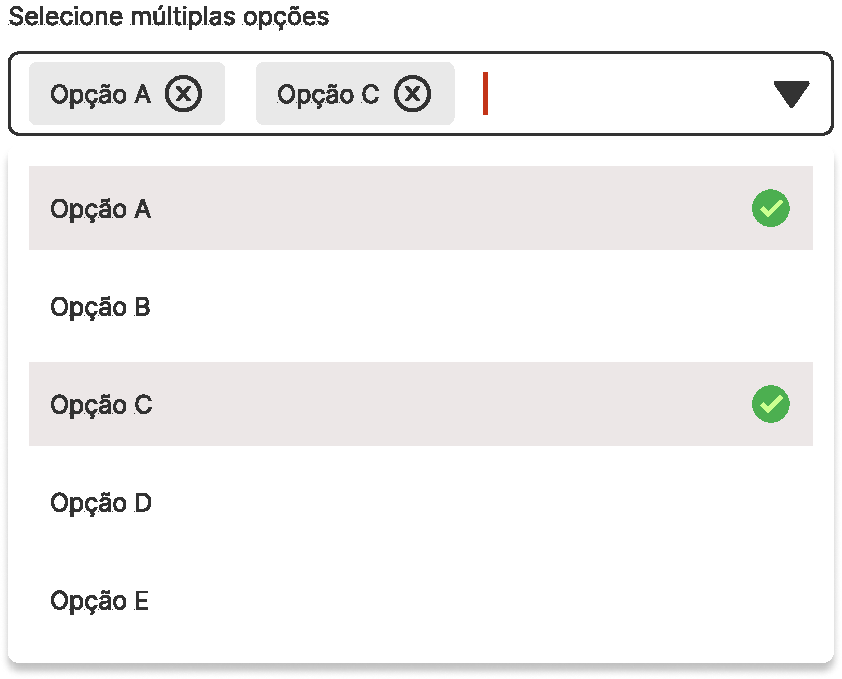
\includegraphics[width=\textwidth]{files/img/2.02!5-desenvolvimento/2.02!5.3-prototipagem/5.3.1-componentes/MultiSelect}
    \caption{Caixa de seleção múltipla} \label{fig:MultiSelect}
  \end{subfigure}
\end{MyCenteredFigure}

A \autoref{fig:selects} mostra os protótipos de caixas de seleção que foram utilizados para a seleção de dados. Na \autoref{fig:SingleSelect} está a caixa de seleção onde o usuário pode selecionar apenas uma opção. Já na \autoref{fig:MultiSelect} a caixa de seleção permite ao usuário selecionar várias opções.

\subsection{Protótipos de páginas} \label{ssec:páginas}                                 % #### 5.3.2

Aqui serão elencadas as sete páginas esboçadas para o sistema. Sendo elas a \hyperref[fig:main]{página principal} (\autoref{fig:main}), a \hyperref[fig:CRUD_main]{página de seleção} (\autoref{fig:CRUD_main}), a \hyperref[fig:CRUD_salas]{página de salas} (\autoref{fig:CRUD_salas}), a \hyperref[fig:CRUD_alunos]{página de alunos} (\autoref{fig:CRUD_alunos}), a \hyperref[fig:CRUD_disciplinas]{página de disciplinas} (\autoref{fig:CRUD_disciplinas}), a \hyperref[fig:CRUD_professores]{página de professores} (\autoref{fig:CRUD_professores}) e a \hyperref[fig:CRUD_turmas]{página de turmas} (\autoref{fig:CRUD_turmas}).

A \textbf{primeira página} é a ilustrada pela \autoref{fig:main} que permite que o usuário arraste todas as turmas listadas até o horário desejado. A listagem das turmas a serem distribuídas é disposta em um painel à esquerda. Este painel tem como funcionalidade, fixar as turmas ainda não alocadas, como se estivessem presas por \LinkToURL{\LinkVelcro}{fechos de gancho e laço}. Assim, dispondo de um local para que turmas em processo de mudança de horário sejam armazenadas temporariamente sem que sejam perdidas.

\begin{MyCenteredFigure} \caption{Protótipo da página principal do sistema} \label{fig:main}
  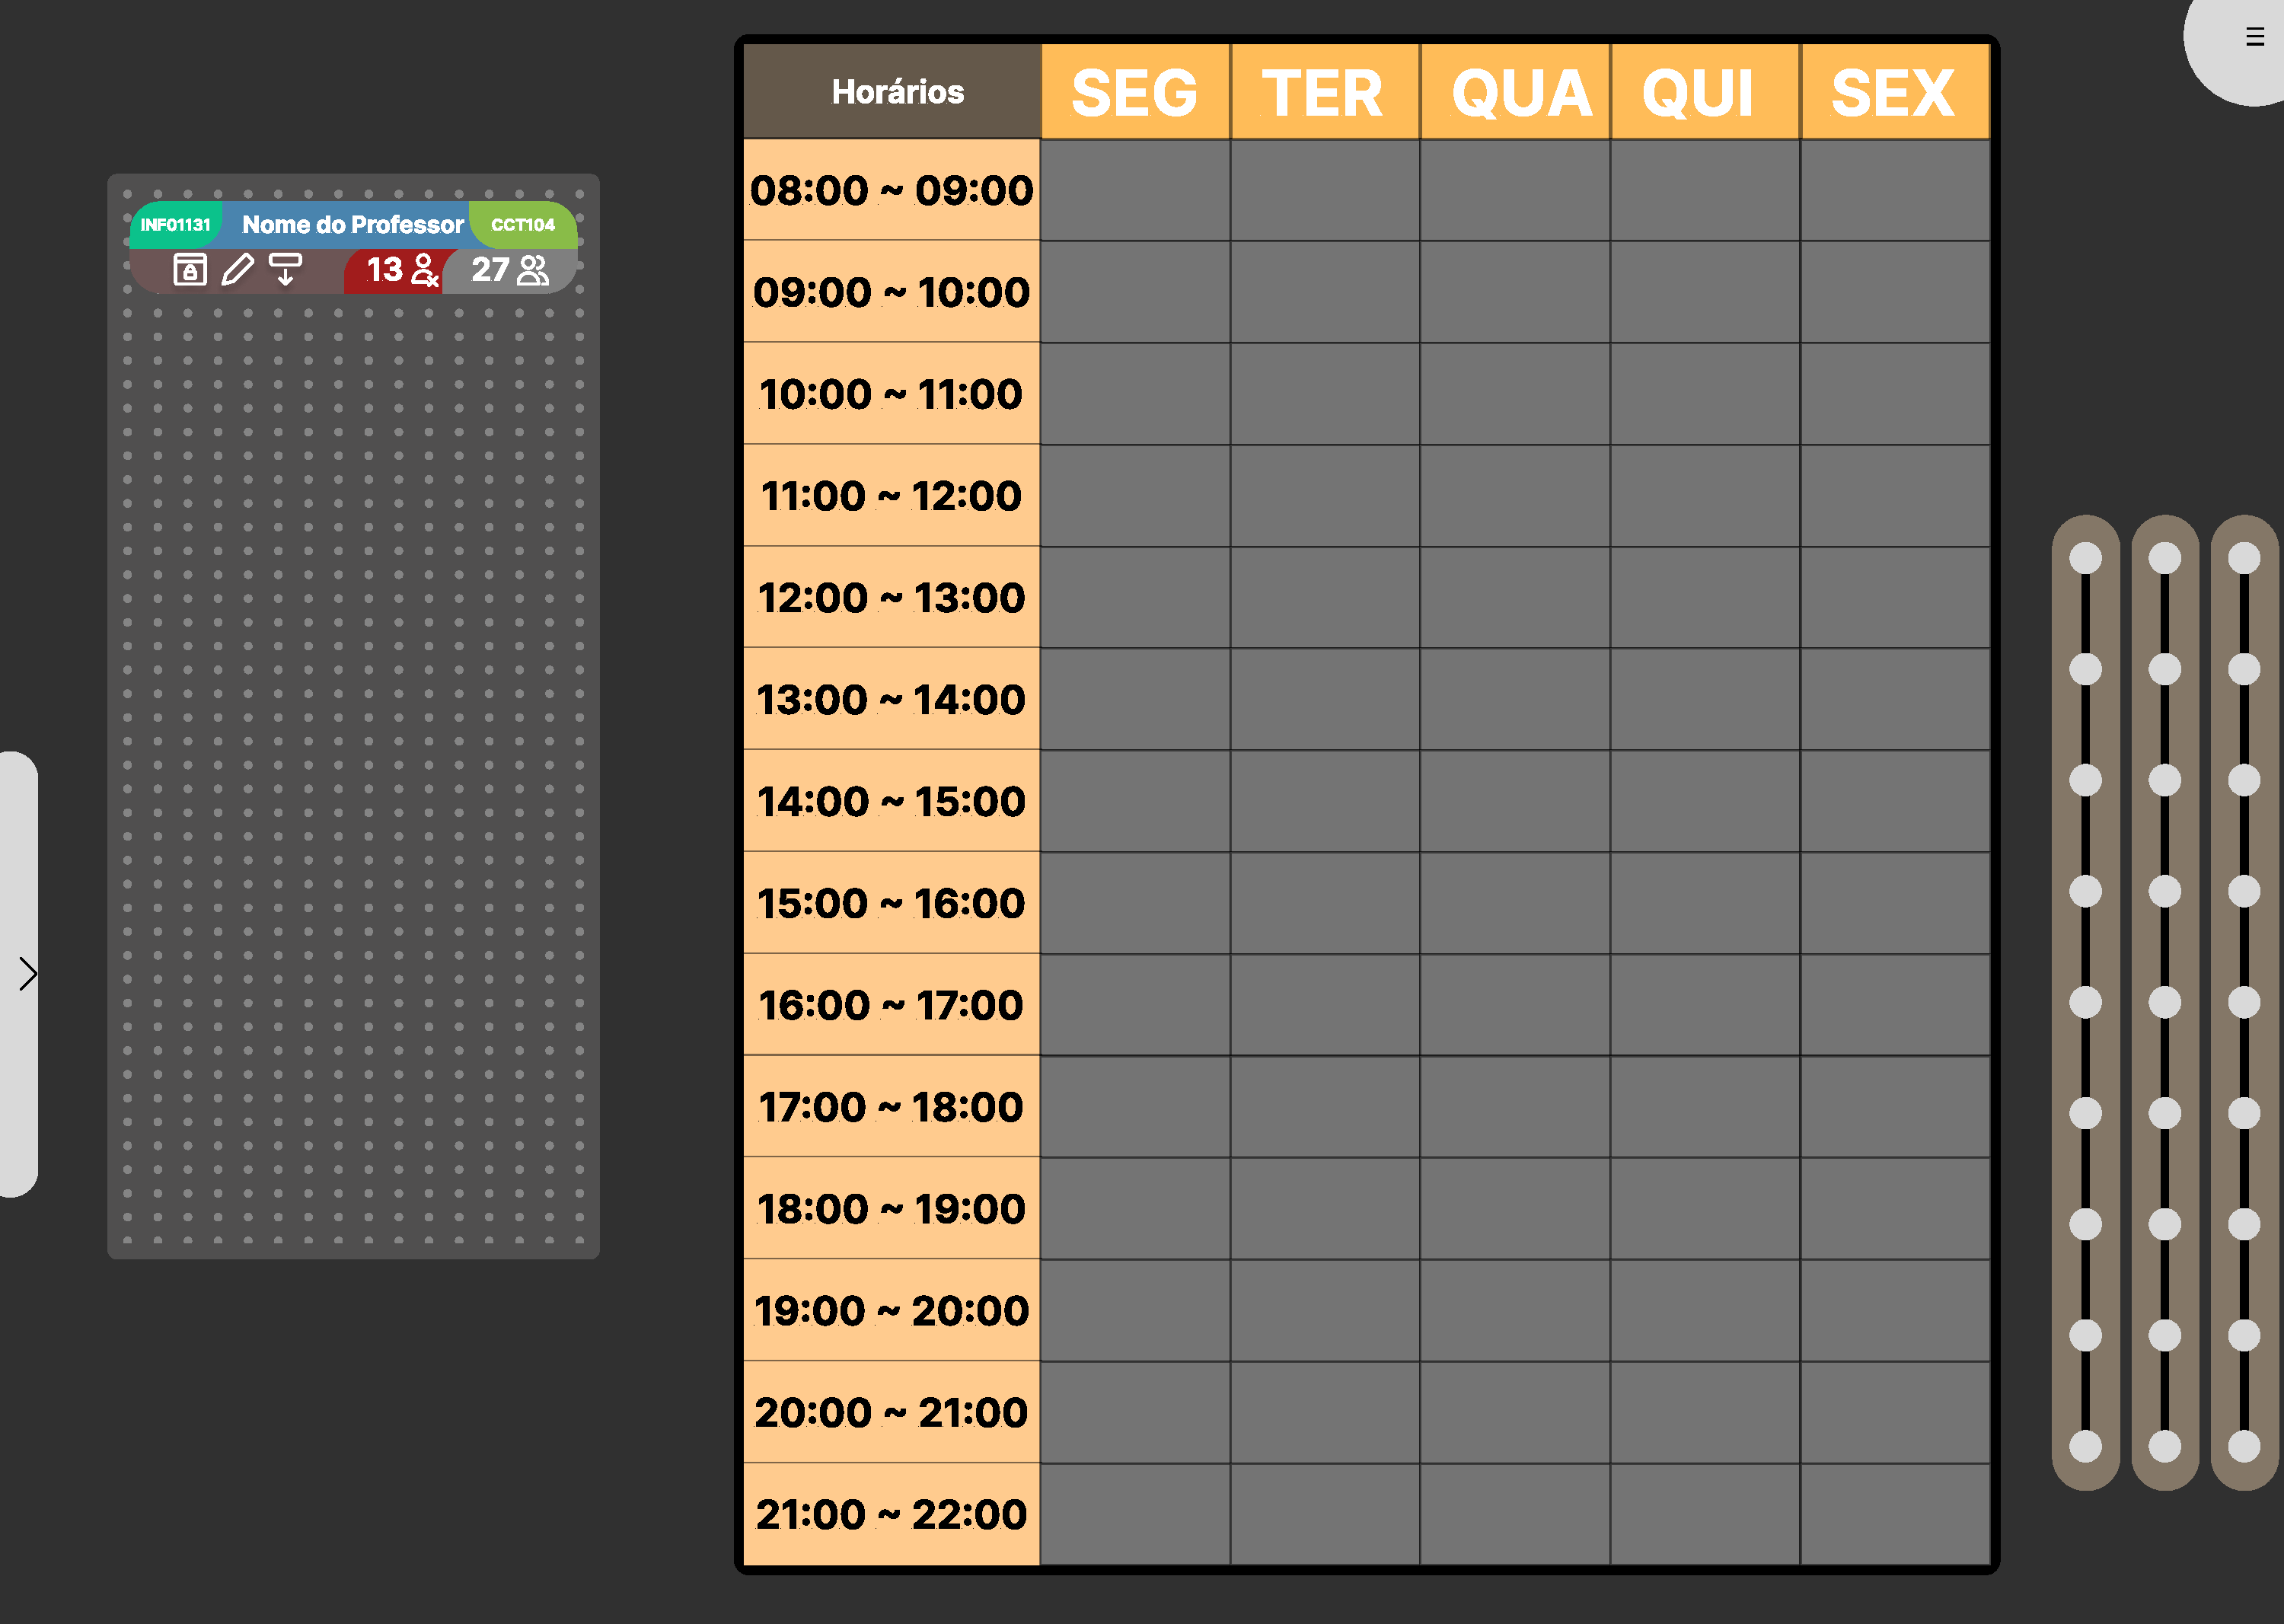
\includegraphics[width=\textwidth]{files/img/2.02!5-desenvolvimento/2.02!5.3-prototipagem/5.3.2-paginas/1-main}
\end{MyCenteredFigure}

Em seguida, temos a \textbf{página de seleção} (\autoref{fig:CRUD_main}) da categoria dos dados que deseja-se modificar, podendo esses serem sobre os professores, alunos, salas, disciplinas ou turmas. Cada uma destas tendo a capacidade de criação, leitura, edição e deleção dos dados.

\begin{MyCenteredFigure} \caption{Protótipo da página de seleção} \label{fig:CRUD_main}
  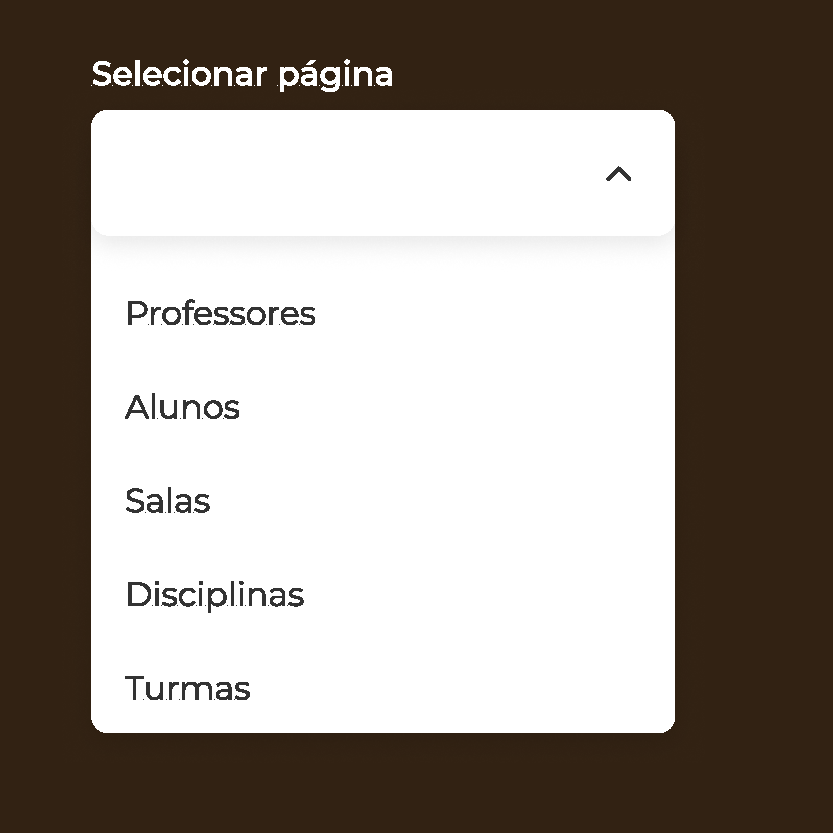
\includegraphics[width=0.5\textwidth]{files/img/2.02!5-desenvolvimento/2.02!5.3-prototipagem/5.3.2-paginas/2-CRUD_main}
\end{MyCenteredFigure}

Quanto à \textbf{página das salas} (\autoref{fig:CRUD_salas}), temos primeiro a seleção da sala na qual deseja-se fazer alterações de cadastro. Abaixo desta caixa de seleção única há um filtro de visualização das alocações de determinado ano e semestre. Nessa página pode-se também registrar algumas características da sala, como a quantidade de cadeiras e computadores, e se possui monitor, projetos, quadro de giz e quadro branco. Um exemplo de sala ainda sem turmas alocadas é representado na \autoref{fig:CRUD_salas}. Essas últimas informações, embora não sejam essenciais para a alocação das turmas, podem ser úteis como forma de filtragem para a alocação de turmas, visto que certas disciplinas demandam salas com características específicas.

\begin{MyCenteredFigure} \caption{Protótipo da página de salas} \label{fig:CRUD_salas}
  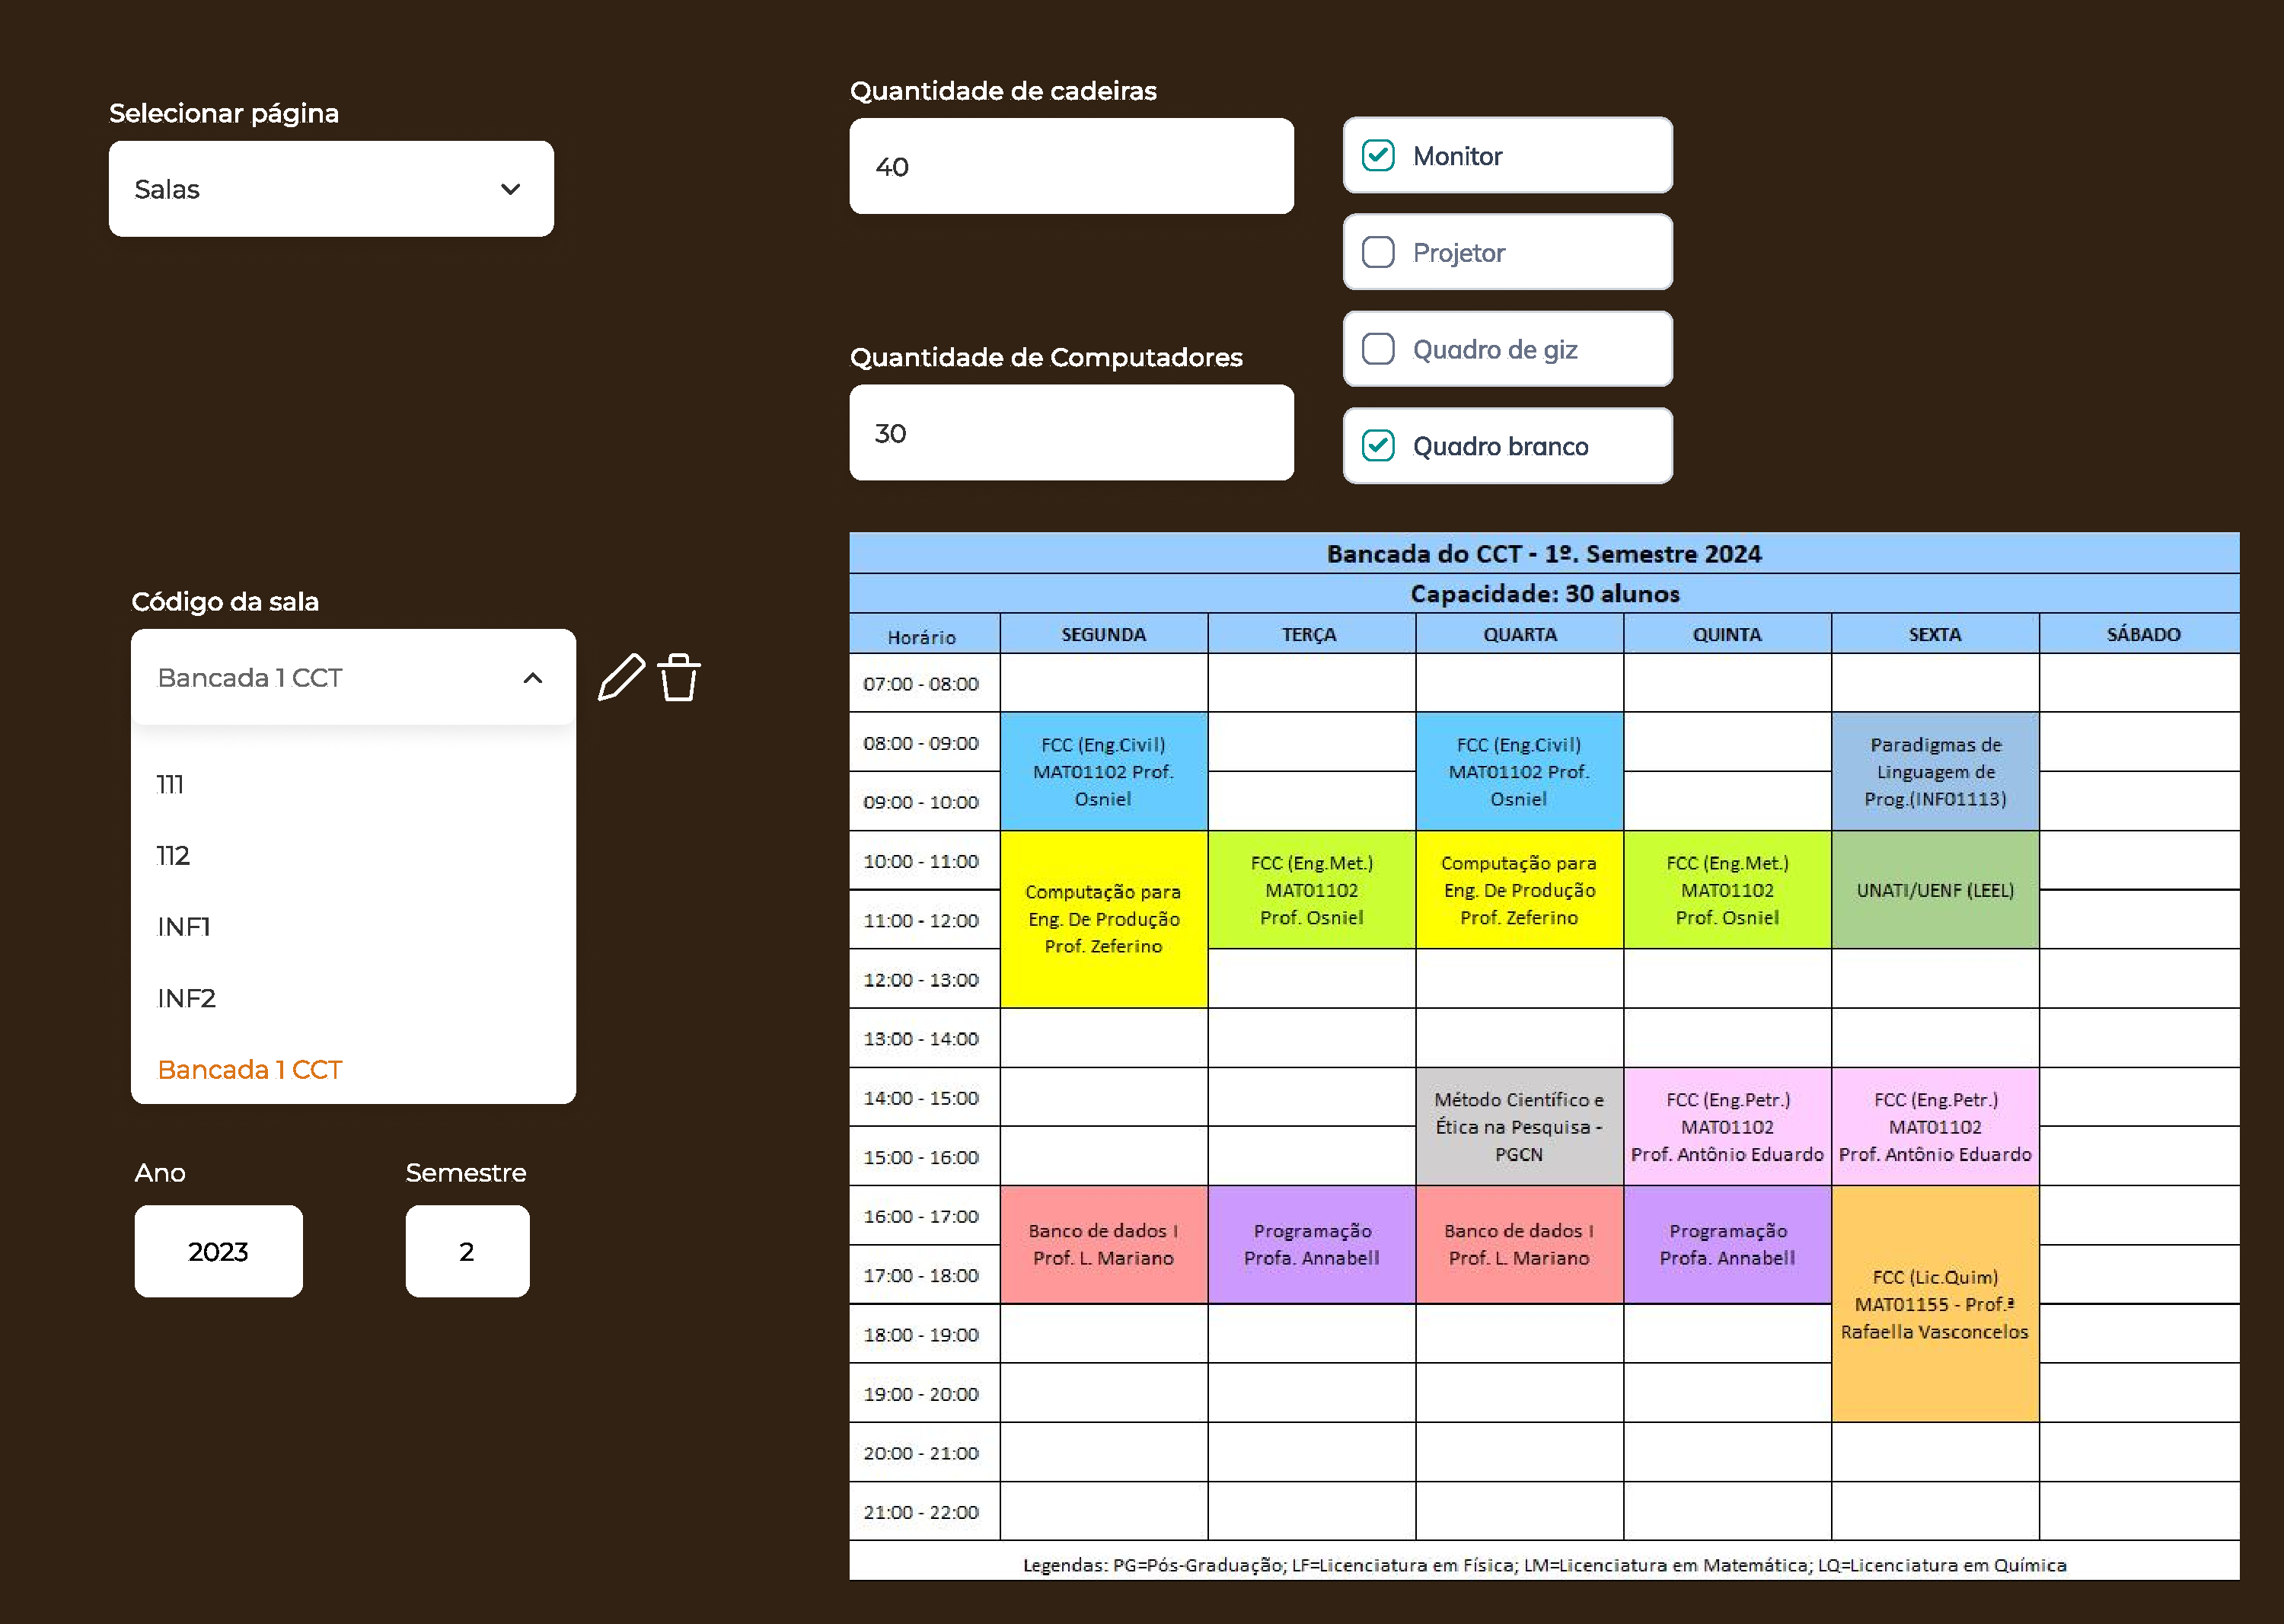
\includegraphics[width=0.9\textwidth]{files/img/2.02!5-desenvolvimento/2.02!5.3-prototipagem/5.3.2-paginas/3-CRUD_salas}
\end{MyCenteredFigure}

Na \textbf{página dos alunos}, pode-se cadastrar novos alunos informando o seu ano de entrada e a sua matrícula. Abaixo temos a visualização da grade, onde pode-se classificar cada uma das disciplinas como aprovada, reprovada e cursando. O exemplo da \autoref{fig:CRUD_alunos} mostra a grade de um aluno inscrito em 2019.1.

\begin{MyCenteredFigure} \caption{Protótipo da página de alunos} \label{fig:CRUD_alunos}
  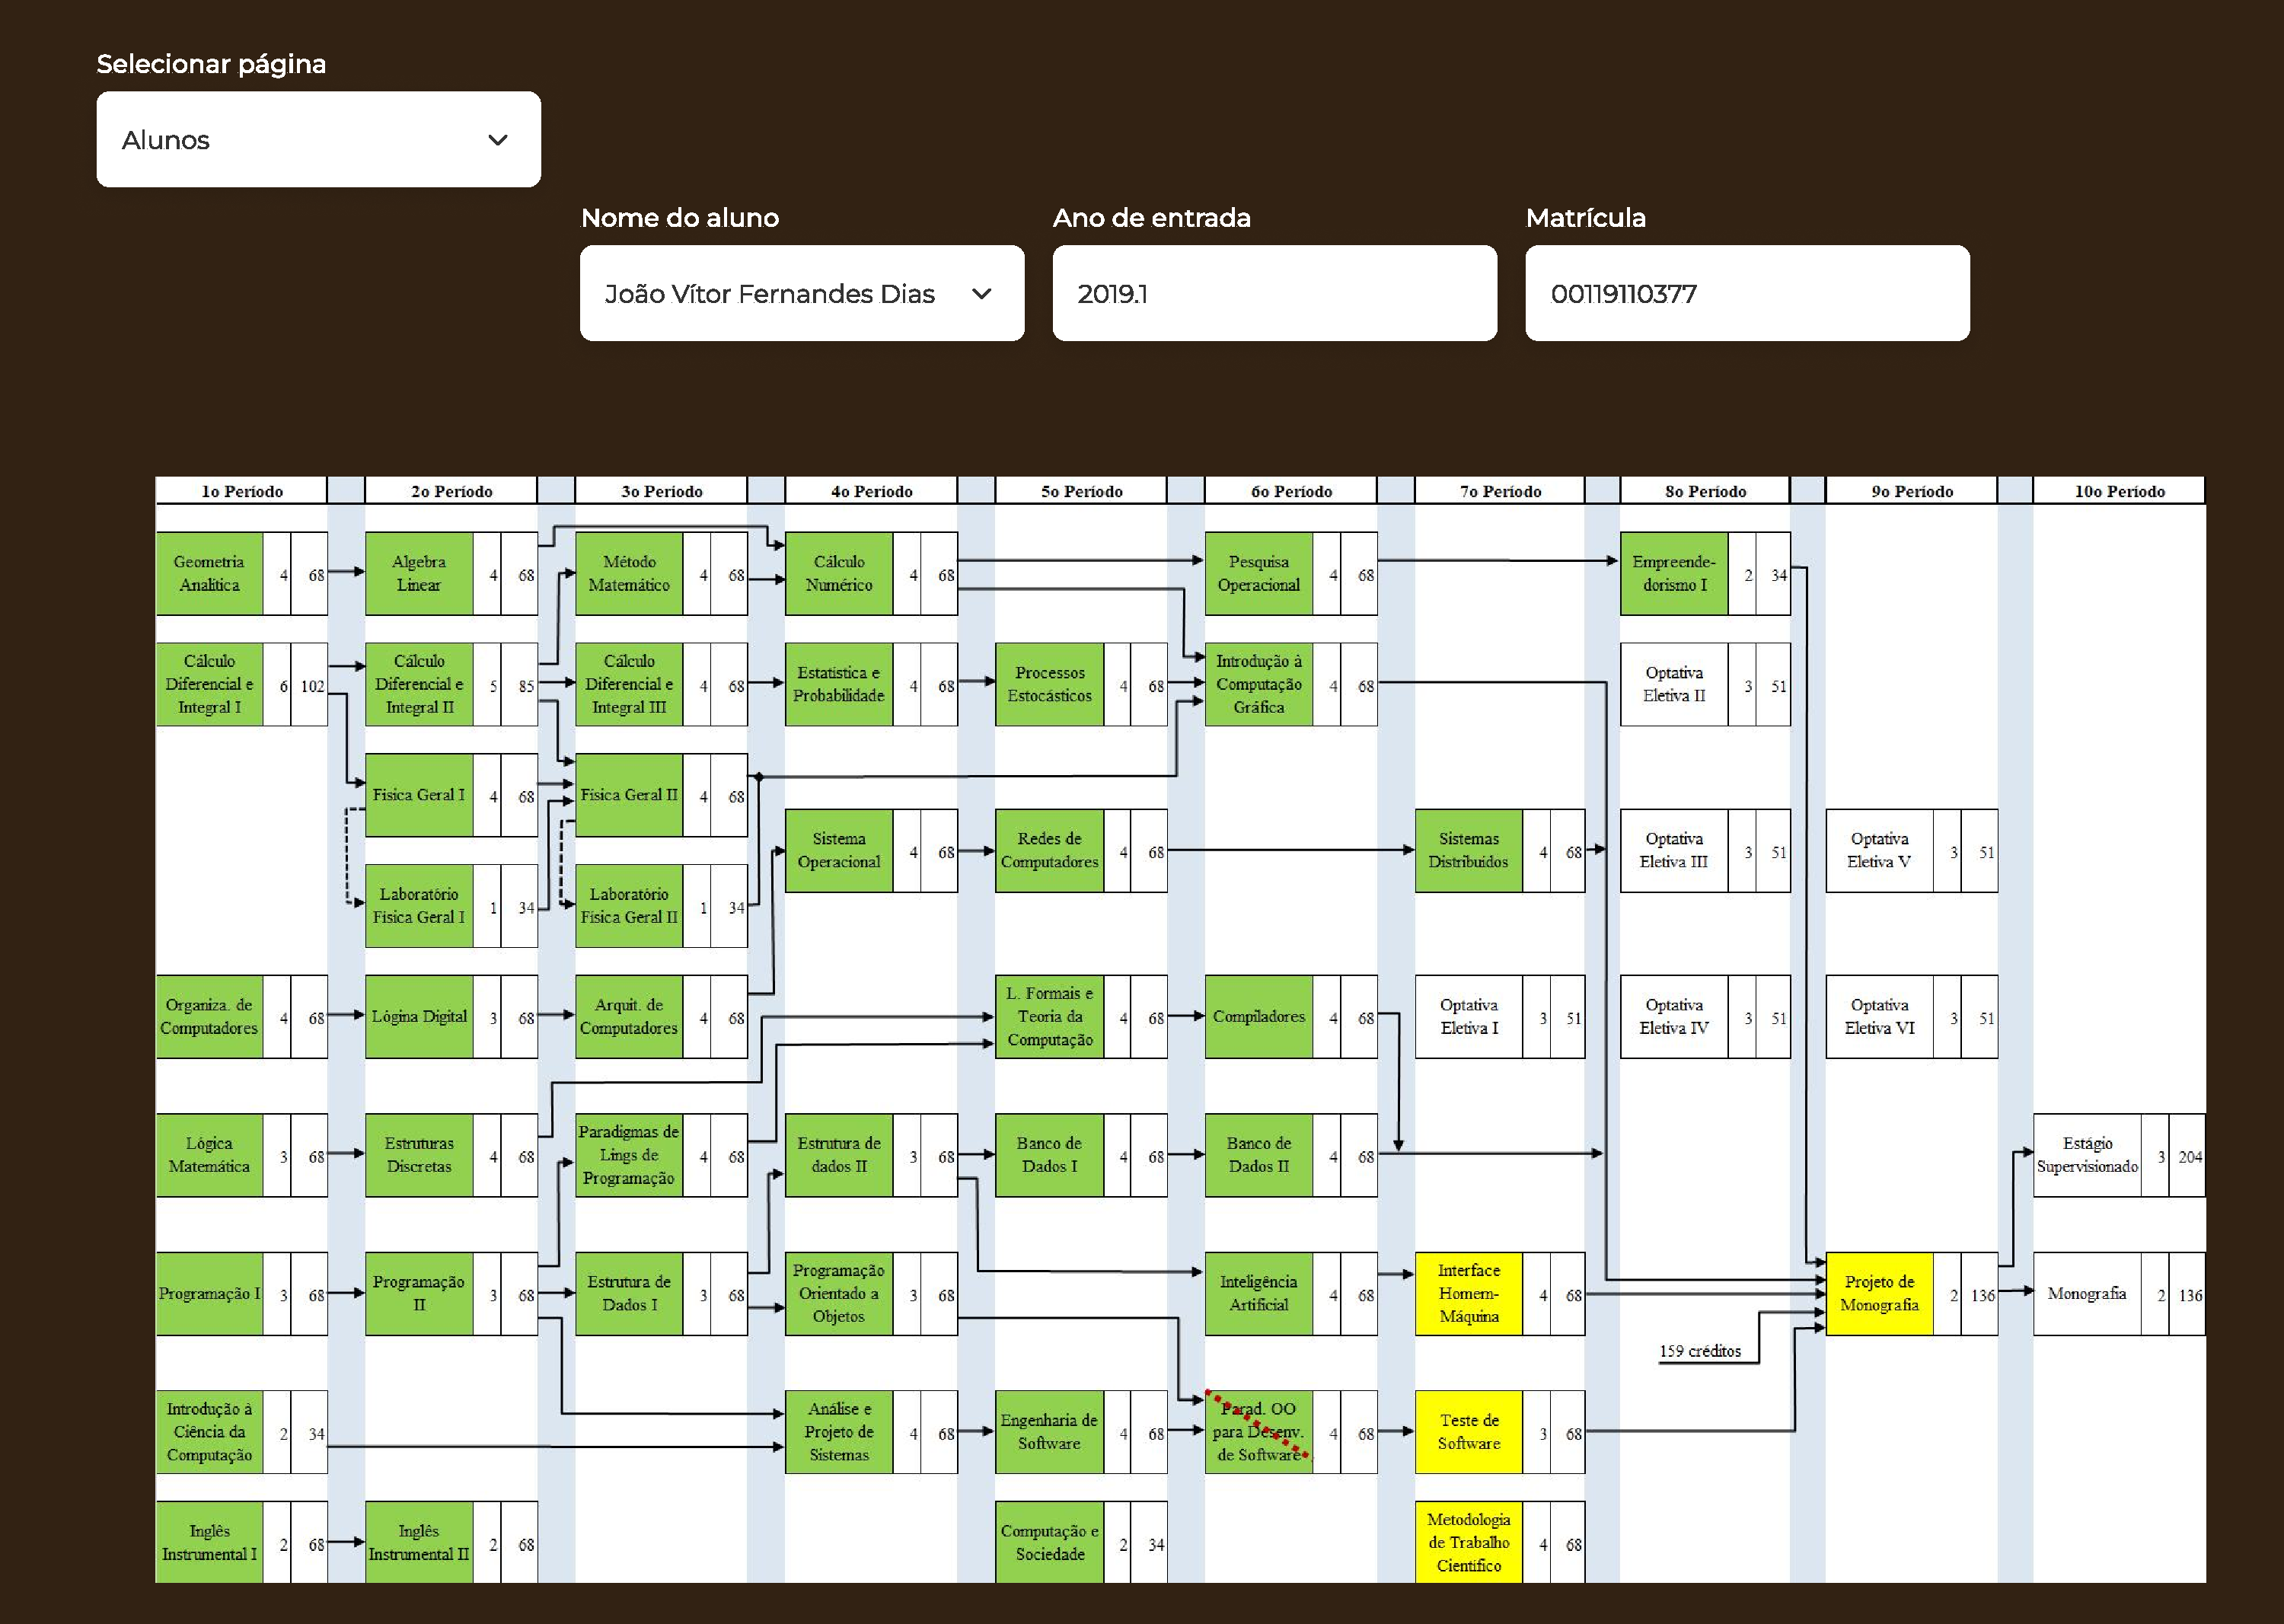
\includegraphics[width=0.9\textwidth]{files/img/2.02!5-desenvolvimento/2.02!5.3-prototipagem/5.3.2-paginas/4-CRUD_alunos}
\end{MyCenteredFigure}

Podemos definir na \textbf{página das disciplinas} qual seu código, nome, e o seu período esperado segundo a matriz curricular. Além dessas informações, pode-se cadastrar quais cursos a possuem em suas matrizes curriculares, quais seus pré-requisitos, os professores que a ministram e quais requisitos a mesma possui em relação às características de sala. A \autoref{fig:CRUD_disciplinas} mostra a página de modificação de disciplinas.

\begin{MyCenteredFigure} \caption{Protótipo da página de disciplinas} \label{fig:CRUD_disciplinas}
  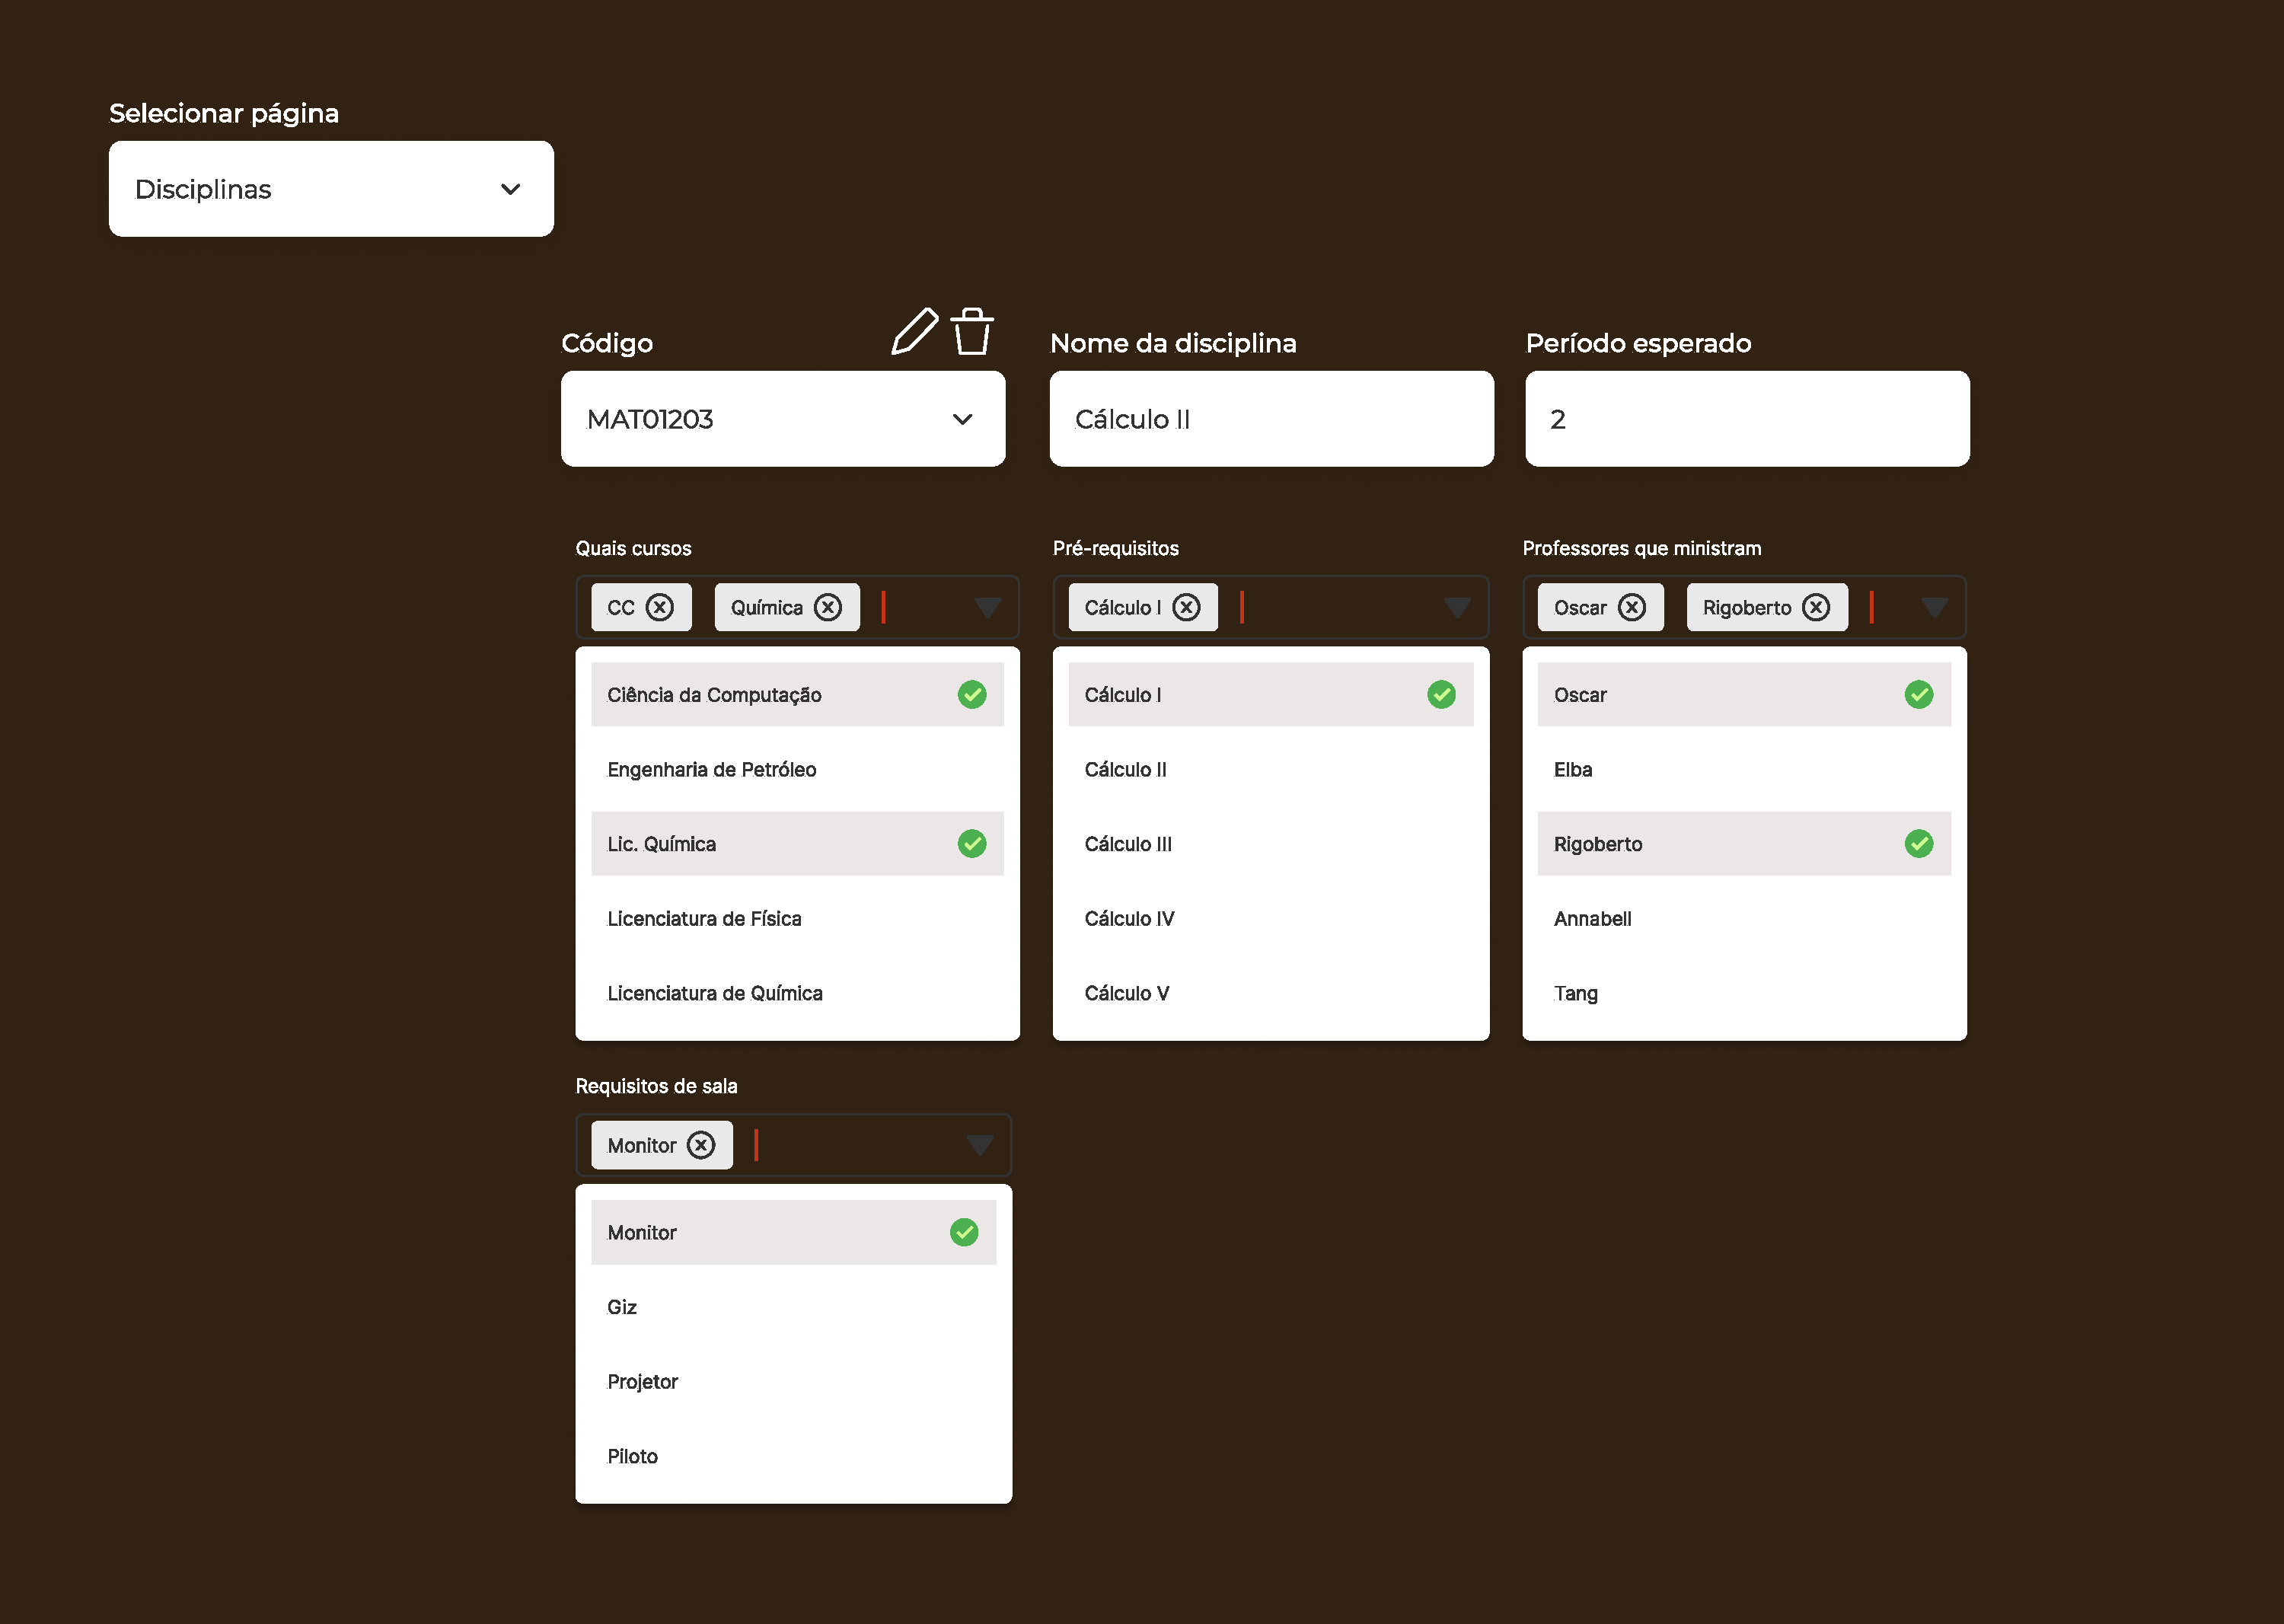
\includegraphics[width=0.8\textwidth]{files/img/2.02!5-desenvolvimento/2.02!5.3-prototipagem/5.3.2-paginas/5-CRUD_disciplinas}
\end{MyCenteredFigure}

Na \textbf{página de professores} (\autoref{fig:CRUD_professores}), temos a relação de disciplinas que os mesmos estão passíveis de ministrar, e também quais são suas preferências de horários ao longo da semana. Embora não seja essencial, essa informação pode ser útil para a alocação de turmas, pois alguns professores podem ter preferência, ou até mesmo não estarem disponíveis para ministrar aulas em determinados horários. Um exemplo deste caso seriam os bolsistas de apoio ao ensino, dado que os mesmos podem estar também vinculados a outras instituições. E nesses casos, aquele que estiver desenvolvendo a grade horária pode alocar as turmas de acordo com a disponibilidade dos professores.

\begin{MyCenteredFigure} \caption{Protótipo da página de professores} \label{fig:CRUD_professores}
  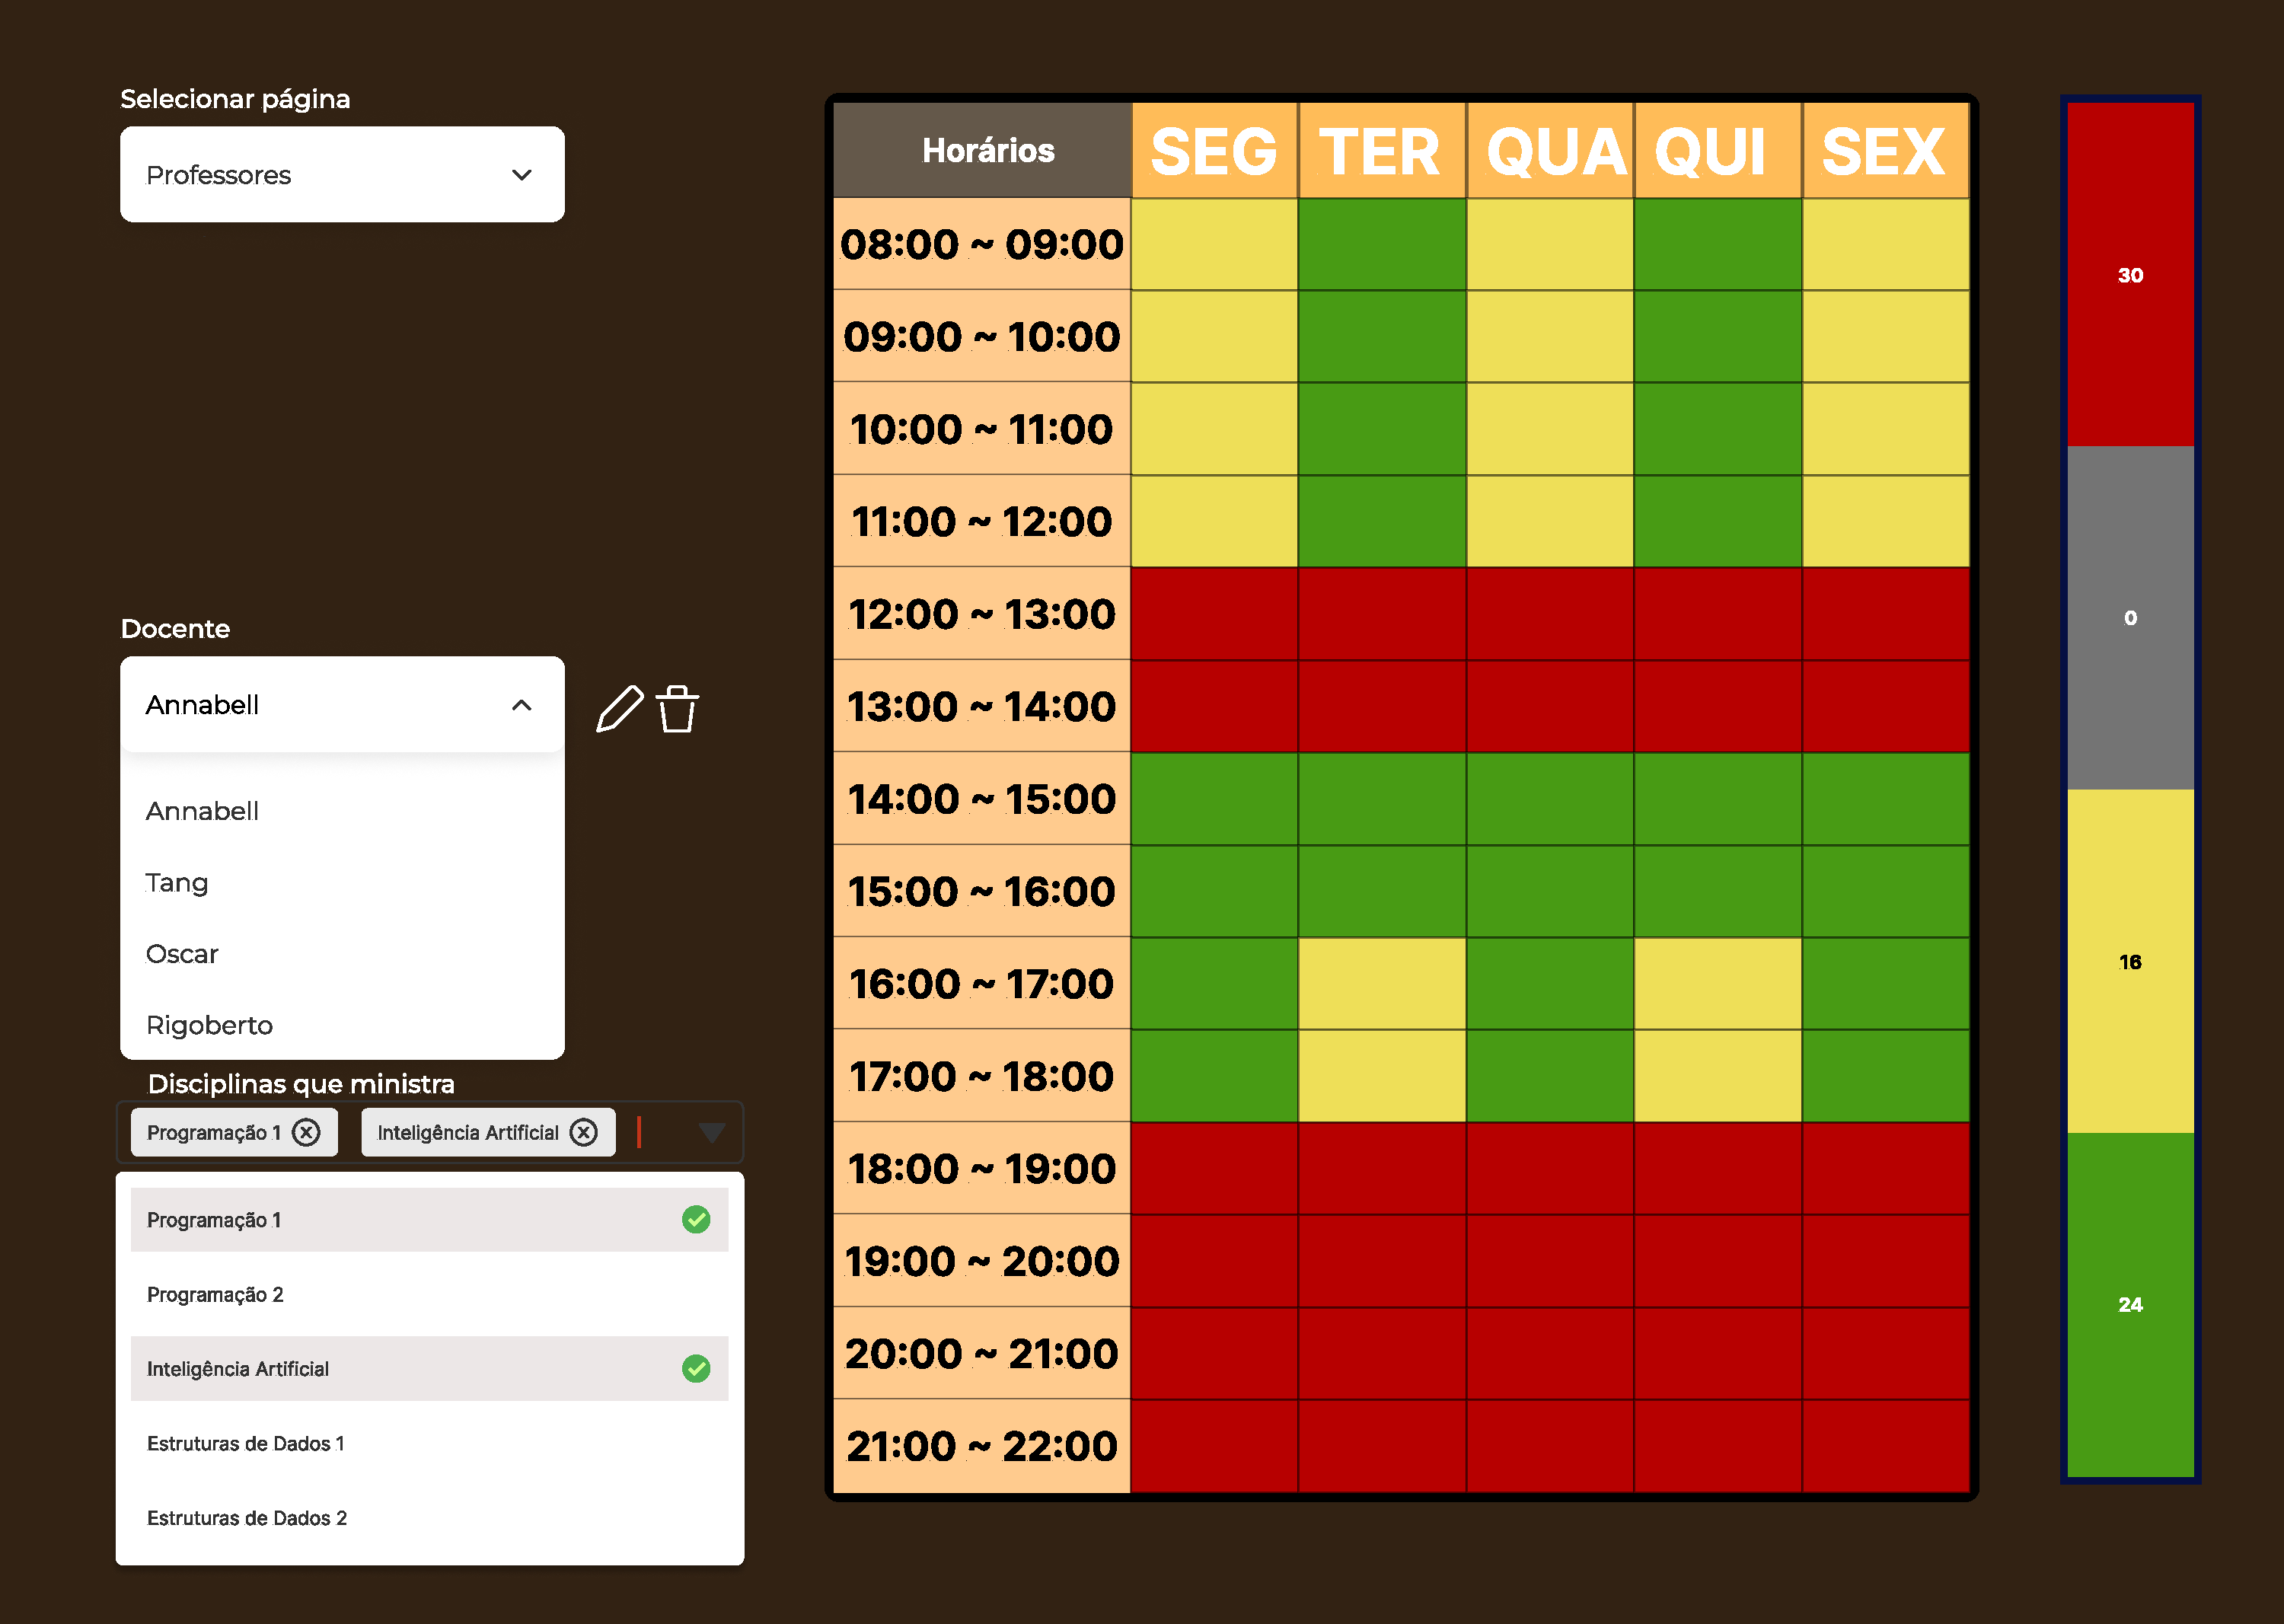
\includegraphics[width=0.8\textwidth]{files/img/2.02!5-desenvolvimento/2.02!5.3-prototipagem/5.3.2-paginas/6-CRUD_professores}
\end{MyCenteredFigure}

Por fim, na \autoref{fig:CRUD_turmas}, temos a junção de todas as informações registradas acima. Nela, podemos alocar os seus horários, definindo o ano, semestre, dia, hora de início e duração em que será ministrada. Também é necessário que seja definido em que sala cada um de seus horários estará alocada. Além de informar, também, qual professor a lecionará e a qual disciplina ela se refere.

\begin{MyCenteredFigure} \caption{Protótipo da página de turmas} \label{fig:CRUD_turmas}
  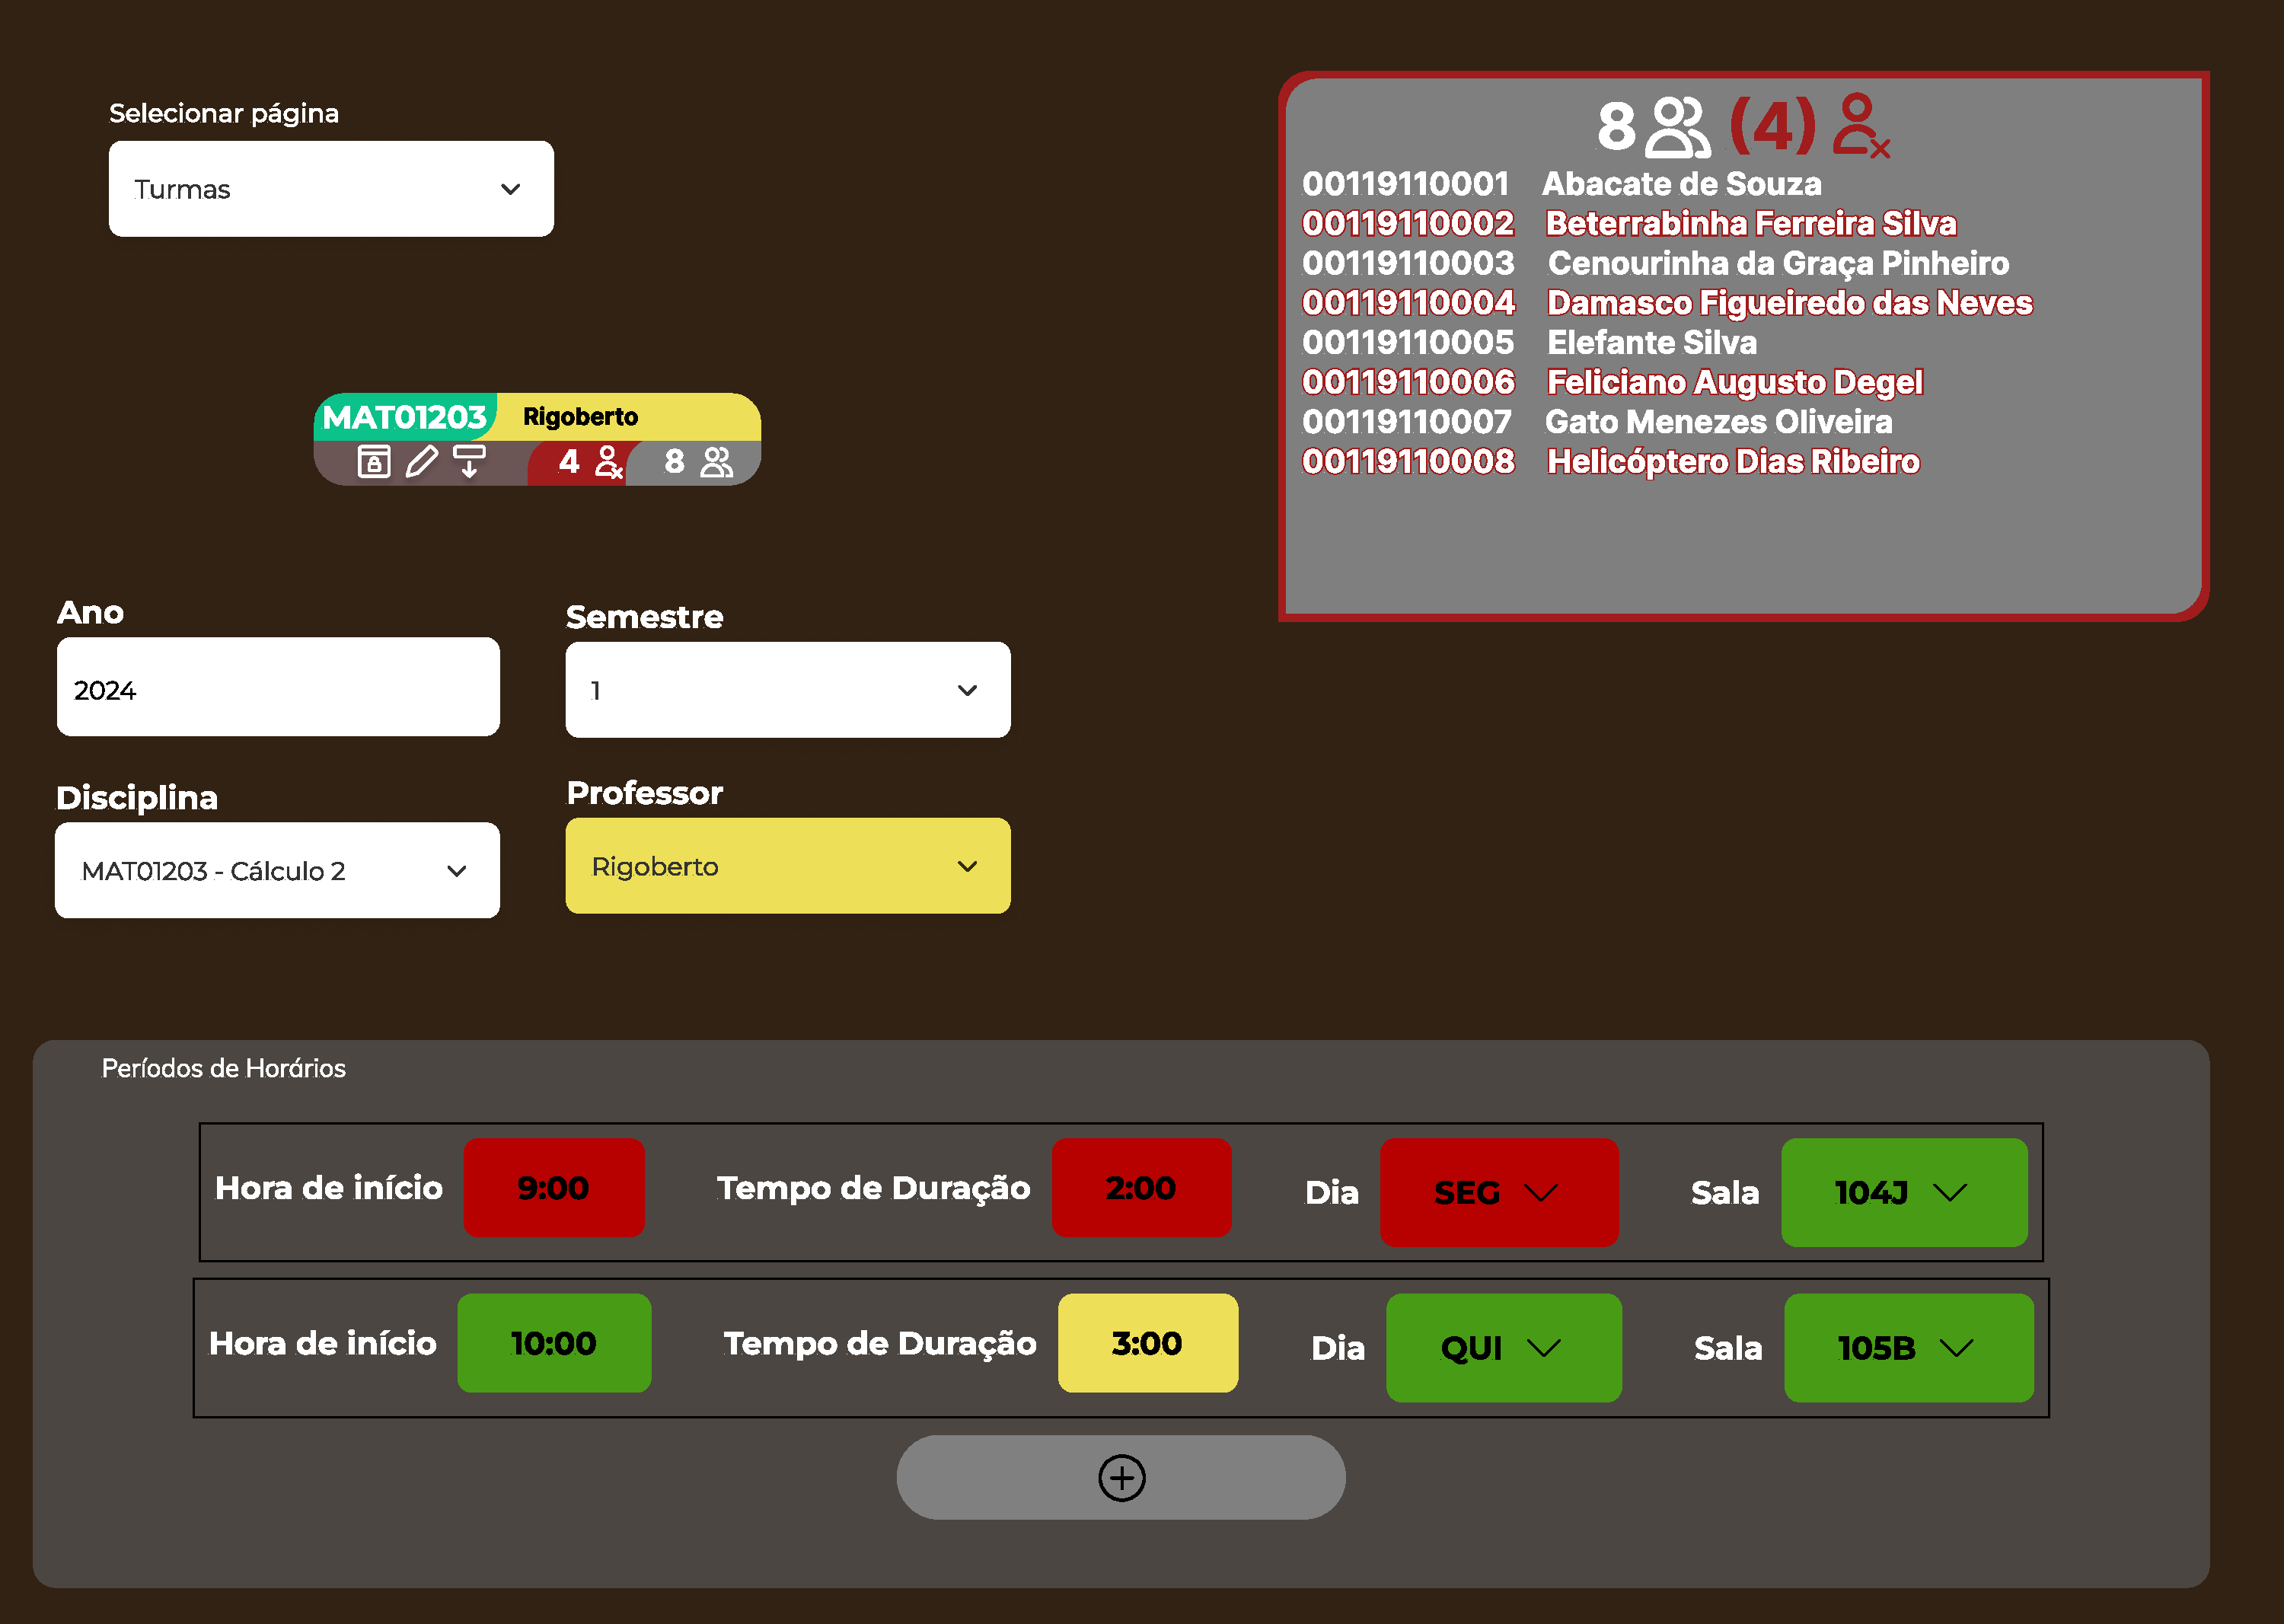
\includegraphics[width=\textwidth]{files/img/2.02!5-desenvolvimento/2.02!5.3-prototipagem/5.3.2-paginas/7-CRUD_turmas}
\end{MyCenteredFigure}

Ainda na \autoref{fig:CRUD_turmas} temos alguns exemplos de conflitos percebidos. O primeiro, com a cor amarelada, informado que o tempo de duração do segundo horário da turma não condiz com a preferência pessoal do professor selecionado. Este conflito não é impeditivo, entretanto, se possível, um outro horário poderia ser encontrado para atender melhor às preferências do professor.

Outro conflito exibido é que a sala em que está alocado o primeiro horário da turma já está ocupada no mesmo horário por outra turma. Este conflito é impeditivo, sendo então representado na cor vermelha. Neste caso, a turma deve ser realocada para outro horário ou sala.

Por último, na listagem dos alunos que podem se inscrever, no canto inferior direito, há quatro alunos marcados em vermelho. Estes alunos poderiam se inscrever em outra turma no mesmo horário em que esta turma está alocada. Este conflito é impeditivo, mas apenas para os alunos, assim como no caso da preferência do professor, a turma pode ser realocada para outro horário para atender melhor às demandas dos alunos.

\section{Programação do sistema} \label{sec:programação}                                % ###  5.4

Após a \hyperref[sec:ModelagemBD]{conceitualização diagramática do banco de dados} e a \hyperref[ssec:componentes]{elaboração dos protótipos com o Figma}, o desenvolvimento do sistema foi iniciado. Por maior familiaridade com a linguagem foi escolhida a linguagem \textbf{\textit{JavaScript}}, utilizando a biblioteca \textbf{\textit{React}} para a criação dos componentes visuais, ou seja, o \textit{frontend}, e o \textbf{\textit{Node.js}} para a criação do \textit{backend} e a criação de um servidor local que permite visualizar as mudanças no código em tempo real. Suas logos estão ilustrados na \autoref{fig:sistemas}.

\begin{MyCenteredFigure} \caption{Recursos usados para o desenvolvimento do sistema} \label{fig:sistemas}
  \begin{animateinline}[loop, autoplay]{1}
    \myAnimation{JavaScript} % 1 JS
    \myAnimation{React}      % 2 React
    \myAnimation{NodeJS}     % 3 Node
    \newframe
    \myAnimation{React}      % 2 React
    \myAnimation{NodeJS}     % 3 Node
    \myAnimation{JavaScript} % 1 JS
    \newframe
    \myAnimation{NodeJS}     % 3 Node
    \myAnimation{JavaScript} % 1 JS
    \myAnimation{React}      % 2 React
  \end{animateinline}
\end{MyCenteredFigure}

% Tang achou esse parágrafo confuso.
Seguindo constantemente o conceito de iteratividade da apresentação do sistema, a programação foi marcada por dois conceitos: blocos de funcionalidades marcantes e blocos de funcionalidades apresentadas. O primeiro conceito se refere à grandes grupos de mudanças que estavam relacionadas a um mesmo tópico, ou que resultaram, quando em conjunto, num sistema consideravelmente distinto de como estava antes de as receber. O segundo conceito se refere à apresentação esporádica da situação atual do sistema para quem o iria utilizar, sendo essas versões chamadas de MVPs (Minimum Viable Product - Mínimo Produto Viável).

Nesta seção serão apresentadas as versões do sistema repartidas de forma a apresentar os agrupamentos de mudanças notórias. Sua \hyperref[sec:programação]{programação} foi repartida em três grandes categorias que visavam entregar o sistema de forma gradual e funcional. A \hyperref[ssec:MVP1]{primeira versão do sistema} foi desenvolvida localmente com o objetivo de se aproximar ao máximo das páginas previstas no protótipo, sem a necessidade de um banco de dados que permitisse alterações. A \hyperref[ssec:MVP2]{segunda versão do sistema} contou com a utilização de duas abordagens distintas de bancos de dados para se obter a permanência dos dados. Já a \hyperref[ssec:MVP3]{terceira versão do sistema} foi desenvolvida de forma a estar completamente hospedada na nuvem, incluindo o seu banco de dados, sendo então \hyperref[sec:preenchimento]{preenchido com mais dados}.

\begin{MyCenteredFigure} \caption{Diagrama da progressão funcionamento da permanência dos dados} \label{fig:API}
  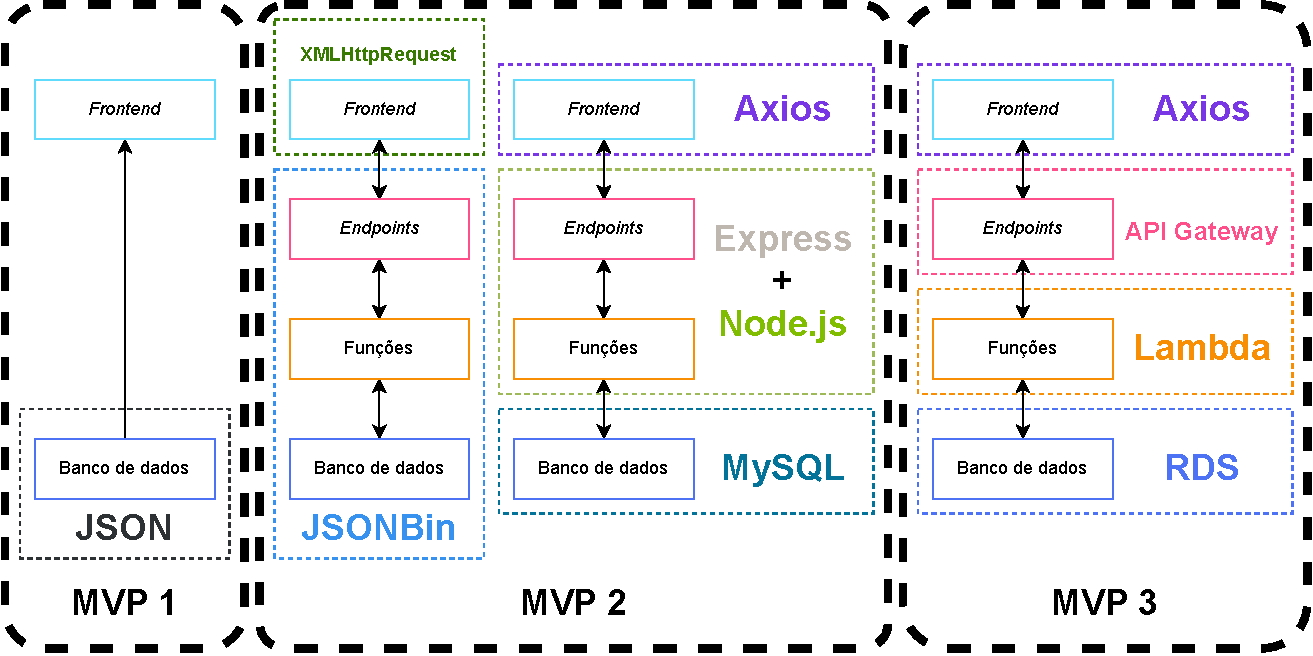
\includegraphics[width=\textwidth]{files/img/2.02!5-desenvolvimento/2.02!5.4-sistema/5.4.0-programacao/API-Progressão}
\end{MyCenteredFigure}

Ao longo da implementação dessas versões, diversos métodos de manutenção dos dados foram utilizados, como a importação de arquivos JSON, a utilização de um banco de dados local e a utilização de um banco de dados hospedado na nuvem. A \autoref{fig:API} ilustra a progressão do funcionamento da permanência dos dados ao longo das três versões do sistema. Os pormenores de cada versão serão descritos adiante.

\subsection{Versão 1.0} \label{ssec:MVP1}                                               % #### 5.4.1

A primeira versão do sistema foi desenvolvida inicialmente em um ambiente local, com o objetivo de se aproximar ao máximo das páginas previstas no protótipo. Para isso, foi utilizada a biblioteca \LinkToURL{\LinkReactRouter}{\textit{React Router}} para a navegação entre as páginas, e a biblioteca \LinkToURL{\LinkReactSelect}{\textit{React Select}} para as caixas de seleção. Ao final desta versão, o sistema foi hospedado no \hyperref[sssec:GitHub Pages]{GitHub Pages} no link \url{\LinkOurClass}.

\subsubsection*{\textbf{Banco de dados preliminar}} \label{sssec:BDInicial}

Os dados contidos no sistema foram inicialmente armazenados em arquivos JSON, que eram importados diretamente para o código (\autoref{fig:API_MVP1}). Isso foi feito para que fosse possível visualizar o funcionamento do sistema sem a necessidade de um banco de dados real. A partir disso, foi possível visualizar o funcionamento do sistema e realizar testes de usabilidade. Em contrapartida, os dados disponíveis não eram modificáveis, tendo apenas a possibilidade de leitura e mutação temporária, visto que após recarregar ou mudar de página, as mudanças eram perdidas.

\begin{MyCenteredFigure} \caption{Diagrama do armazenamento preliminar dos dados} \label{fig:API_MVP1}
  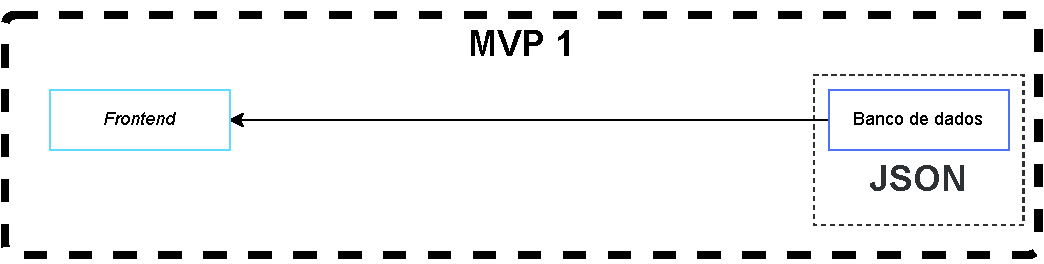
\includegraphics[width=\textwidth]{files/img/2.02!5-desenvolvimento/2.02!5.4-sistema/5.4.1-MVP1/API_MVP1}
\end{MyCenteredFigure}

Nesse método, cada entidade era armazenada em um arquivo JSON separado, contendo esse um array de objetos, onde em cada objeto haviam as chaves, representando as propriedades da entidade, e os valores, representando os dados da entidade.

Como nesta dinâmica não havia uma forte correlação entre os dados, o \textit{frontend} acabava sendo o responsável por unir todas as informações. Assim, por exemplo, para se obter a lista de professores de uma turma, era necessário importar todos os professores, todas as turmas, e então, a partir do nome do professor alocado àquela turma, buscar na listagem dos professores qual era o professor que correspondia àquele nome, para então agregar as informações.

\subsubsection*{\textbf{Funcionalidades iniciais: CRUD e primeiros conflitos}} \label{sssec:Funcionalidades Iniciais}

Nessa primeira versão, algumas funcionalidades já começaram a ser esboçadas, principalmente as funcionalidades CRUD (\textit{Create}, \textit{Read}, \textit{Update}, \textit{Delete}) para as entidades principais do sistema. Embora, como já dito, os dados não fossem persistentes, foi possível visualizar o funcionamento das funcionalidades de criação e leitura de turmas, professores, disciplinas, salas e horários.

Nessa versão, também foi implementada uma checagem bruta de conflitos por alocação simultânea de professores em mais de uma turma e a checagem da quantidade de demanda de alunos em relação à capacidade das salas. Uma descrição mais detalhada das funcionalidades de conflitos está presente adiante na \autoref{sec:conflitos} denominada \nameref{sec:conflitos}.

\subsubsection*{\textbf{Preferências dos professores, progressão dos alunos e recursos da sala}} \label{sssec:Progressão dos Alunos e Preferência dos Professores}

Além das funcionalidades citadas anteriormente que se mantiveram até a conclusão do sistema, também foram desenvolvidas funcionalidades que não obtiveram o mesmo êxito e que foram deixadas de lado. Dentre elas, podemos citar a definição de níveis de \textbf{preferência de horários para professores}, a \textbf{progressão dos alunos} em relação às disciplinas, e a definição das \textbf{características especiais das salas}.

A tabela de preferências de horários para professores foi desenvolvida e consistia em permitir a definição de níveis de preferência para cada um dos horários da semana. A ideia era que, ao alocar as turmas, o sistema pudesse priorizar os horários que fossem mais bem avaliados pelos professores, assim aumentando sua satisfação sempre que possível. A funcionalidade foi descartada por ser considerada de menor prioridade em relação a outras funcionalidades, segundo a coordenação de computação, não sendo ela um dos fatores mais relevantes para a definição das grades horárias no curso de Ciência da Computação.

\subsubsection*{\textbf{GitHub Pages}} \label{sssec:GitHub Pages}

Após o desenvolvimento local foi feita a implementação da interface do sistema para um servidor online. Para isso, foi utilizado o serviço \LinkToURL{\LinkGitHubPages}{GitHub Pages} que, por ser gratuito e de fácil utilização, foi a escolha mais adequada para o momento.

Para implantar no GitHub Pages o código desenvolvido, utilizou-se da \LinkToURL{\LinkBibliotecaGHPages}{biblioteca gh-pages}, que viabiliza a publicação de um site diretamente do repositório do GitHub. A partir disso, o sistema foi disponibilizado para acesso público, permitindo que qualquer pessoa pudesse acessar o sistema e testar suas funcionalidades no endereço eletrônico \url{\LinkOurClass}.

\subsection{Versão 2.0} \label{ssec:MVP2}                                               % #### 5.4.2

Utilizando do \textit{feedback} quanto aos resultados entregues na \hyperref[ssec:MVP1]{primeira versão}, alguns pontos de melhoria foram identificados, sendo um deles, e o mais importante: o planejamento. Na primeira abordagem, o desenvolvimento foi feito seguindo notas e ideias soltas, sem um planejamento prévio, o que resultou em um sistema que, embora funcional, não atendia a todas as necessidades propostas. Também dispunha de funcionalidades que não eram de todo necessárias, ou, melhor dizendo, que tinham menor prioridade do que muitas outras. Como solução, foi utilizado o \hyperref[sssec:GitHub Projects]{GitHub Projects} para organizar as tarefas e priorizá-las.

% Mesmo com esta nova dinâmica, outras funcionalidades foram deixadas de lado. Uma das que foram deixadas de lado foi a possibilidade de fixar certas informações. A proposta era que, certas disciplinas que são ofertadas para múltiplos cursos, pudessem ser fixadas em horários específicos, para que simplificasse aos criadores de grades horárias a alocação de turmas.

% Nessa versão, também foram utilizados dois métodos de manutenção dos dados o \hyperref[ssssec:JSONBin]{JSONBin} que não atingiu às expectativas e o \hyperref[ssssec:MySQL]{MySQL} que serviu para a criação de um banco de dados local, já emulando o \hyperref[sssec:Amazon Web Services]{posterior uso de um banco de dados hospedado na nuvem}.

Seguindo o planejamento feito, uma das primeiras tarefas foi a implementação do banco de dados que permitisse a \hyperref[sssec:Permanência dos Dados]{permanência dos dados}, para isso, foram utilizados dois métodos de manutenção dos dados: o \hyperref[ssssec:JSONBin]{JSONBin} e o \hyperref[ssssec:MySQL]{MySQL}. Outro ponto foi a criação da \hyperref[sssec:Logomarca]{logomarca} do sistema, que foi feita para que o sistema tivesse uma identidade visual própria. Foram desenvolvidas também \hyperref[sssec:Funcionalidades Adicionais]{algumas outras funcionalidades}, como a análise de conflitos adicionais, a possibilidade de se filtrar as turmas e a visualização de disciplinas que ainda não têm uma turma criada no semestre em planejamento.

\subsubsection*{\textbf{GitHub Projects}} \label{sssec:GitHub Projects}

Utilizando o \LinkToURL{\LinkGitHubProjects}{GitHub Projects}, foi organizada uma tabela de tarefas, vista na \autoref{fig:GitHubProjectsTable}, onde foram unificadas as diversas anotações e ideias, antes soltas. A partir disso, foi possível visualizar o que era mais importante e o que poderia ser deixado de lado.

\begin{MyCenteredFigure} \caption{Tabela de tarefas do GitHub Projects} \label{fig:GitHubProjectsTable}
  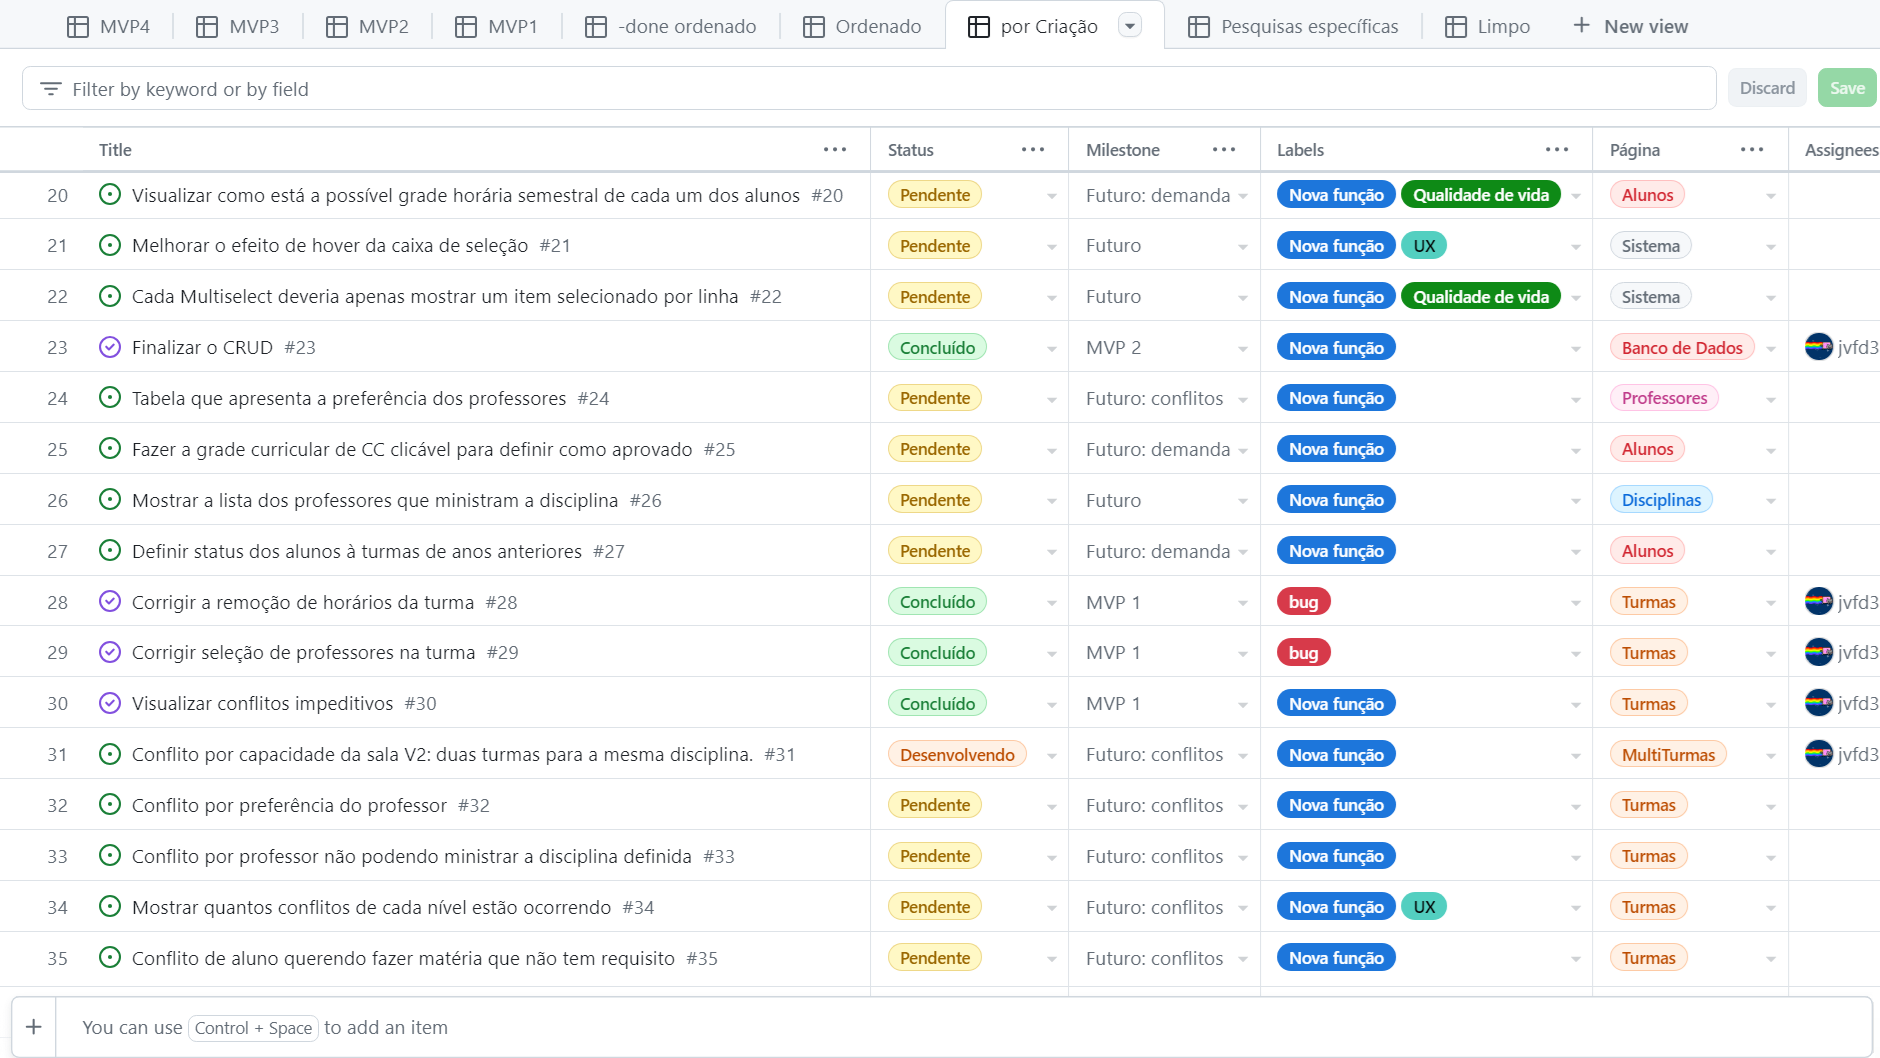
\includegraphics[width=\textwidth]{files/img/2.02!5-desenvolvimento/2.02!5.4-sistema/5.4.2-MVP2/GitHubProjects-Table-Light}
\end{MyCenteredFigure}

Tendo este novo sistema de tarefas em prática, foi possível planejar melhor quais eram as funcionalidades que precisavam ser desenvolvidas, as que já estavam prontas, as que poderiam ter melhorias e quais se desejava implementar no futuro.

As tarefas foram inicialmente divididas em três principais categorias: \textit{Status}, \textit{Página} e \textit{Sequência}. O \textit{Status} reflete o andamento do código da tarefa, podendo ser este andamento \textbf{Pendente}, \textbf{Desenvolvendo}, ou \textbf{Concluído}. A \textit{Página} reflete em qual página do sistema a tarefa se encontra, e a \textit{Sequência} reflete a ordem de prioridade da tarefa.

Citando mais detalhes da \autoref{fig:GitHubProjectsTable}, temos à esquerda a numeração das tarefas, seguido do título da tarefa que descreve em poucas palavras sobre o que se trata. ao final do título há uma combinação do símbolo ``\#'' e uma numeração. Essa numeração representa a sequência de criação das tarefas, código esse que pode ser usado como referência entre as tarefas, assim permitindo que tarefas correlacionadas tenham um link direto entre elas. Na próxima coluna está o \textit{Status} da tarefa, seguido de duas colunas, \textbf{\textit{Milestone}} e \textbf{\textit{Labels}} que só foram criadas \hyperref[ssssec:Marcos e Etiquetas]{posteriormente}. Finalizando temos a coluna \textbf{Página} que primariamente distingue em qual página do sistema a tarefa se encontra, mas que também contém algumas categorias que fogem do conceito de página, como por exemplo é o caso das categorias ``Componente'', ``Sistema'' e ``Banco de Dados''. Por último há a coluna \textit{Assignees} que indica quem é o responsável pela tarefa; nesse caso, todas as tarefas que estão em andamento ou que já se encontram concluídas foram atribuídas ao mesmo responsável.

\subsubsection*{\textbf{Permanência na alteração dos dados}} \label{sssec:Permanência dos Dados}

Tendo agora uma rota mais clara a ser seguida, o desenvolvimento foi retomado. Uma das características mais marcantes e ainda não atribuídas ao sistema era a manutenção das modificações feitas nos dados. Nesta etapa, foram utilizados dois métodos de se manter as alterações feitas aos dados. Com esse intuito foram utilizados dois métodos de manutenção dos dados o \hyperref[ssssec:JSONBin]{JSONBin} que não atingiu às expectativas e o \hyperref[ssssec:MySQL]{MySQL} que serviu para a criação de um banco de dados local, já emulando o posterior uso de um \hyperref[sssec:Amazon Web Services]{banco de dados hospedado na nuvem}. Como nessa etapa houveram esses dois métodos de manutenção dos dados, a \autoref{fig:API_MVP2} ilustra o paralelo entre os dois métodos.

\begin{MyCenteredFigure} \caption{Comparação entre bancos de dados da Versão 2.0} \label{fig:API_MVP2}
  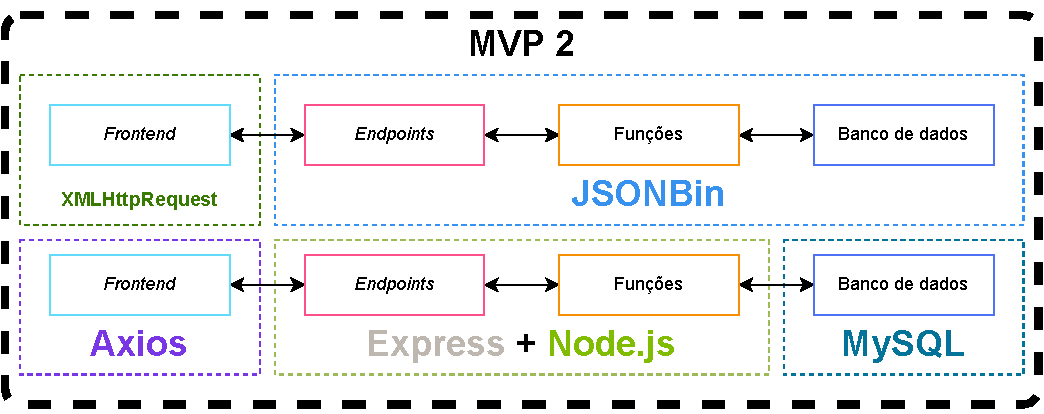
\includegraphics[width=\textwidth]{files/img/2.02!5-desenvolvimento/2.02!5.4-sistema/5.4.2-MVP2/API_MVP2}
\end{MyCenteredFigure}

\subsubsubsection*{A) \LinkToURL{\LinkJSONBin}{JSONBin}} \label{ssssec:JSONBin}

Como até então os dados estavam armazenados em formato JSON, imaginou-se que a melhor forma de persistir os dados seria através de um banco de dados que lidasse com JSON, o escolhido para este fim foi o JSONBin por apresentar ser uma plataforma gratuita e de fácil utilização.

Esta plataforma permite a criação de \textit{bins}, que são basicamente coleções de dados em formato JSON. A partir disso, é possível realizar requisições HTTP para a leitura, escrita, atualização e remoção dos dados. A utilização do JSONBin foi feita através de requisições HTTP usando o objeto \textit{XMLHttpRequest} do JavaScript, e a comunicação entre o \textit{frontend} e o JSONBin foi feita através de \textit{tokens} de acesso. Este fluxo é representado pela seção superior da \autoref{fig:API_MVP2}.

Com isso, se tornou possível ler e atualizar os dados de forma remota, e assim, manter os dados mesmo após a recarga da página. Embora cumprisse com o que promete e o que era desejado, o JSONBin não se mostrou a melhor escolha para o sistema, visto que a sua utilização não performou tão bem quanto se esperava.
% Não se sabe se foi por inexperiência ou por limitações do próprio serviço, mas
A utilização do JSONBin para a coleta dos dados, fazia com que a tela de carregamento do sistema demorasse alguns segundos para ser exibida, o que não é apropriado para a usabilidade do sistema proposto.

\subsubsubsection*{B) \LinkToURL{\LinkMySQL}{MySQL}} \label{ssssec:MySQL}

Embora houvesse o desejo do uso de informações em formato JSON, achou-se por bem utilizar um banco de dados mais usual, recorrendo então ao MySQL, sendo então necessário criar um banco de dados local que armazenasse os dados e que pudesse ser acessado pelo sistema. Essa configuração serviu para estabelecer a supracitada camada de banco de dados. E consistiu basicamente na instalação do MySQL Server.

\paragraph*{B1) Migração dos dados}

Como os dados se encontravam em formato JSON, primariamente utilizou-se da ferramenta de importação de dados do próprio \textbf{MySQL Workbench}. Durante essa importação, o software automaticamente identifica os campos, criando a tabela e suas colunas. Porém, devido à quantidade dos dados, essa importação tendia a ser demorada, e por vezes, falhava
% , sem haver uma explicação clara do porquê
.

Com isso, foi necessário recorrer a uma abordagem semimanual, sendo então desenvolvido um código em Python que lê os arquivos JSON e os converte em arquivos SQL para que as \textit{queries} pudessem ser executadas no MySQL Workbench. A partir disso, foi possível importar os dados de forma mais rápida e eficiente.

Apesar da primeira tentativa de importação não ter sido completamente bem sucedida, foi desta forma que as tabelas, representadas pela \autoref{fig:TabelasIniciais}, foram inicialmente criadas. Isso gerou posteriormente a necessidade de ajustes manuais, como a adição de chaves primárias e estrangeiras, e a alteração de tipos de dados. Porém, como neste momento, o sistema visava apenas replicar o funcionamento do JSONBin, essas alterações não foram feitas de imediato.

\begin{MyCenteredFigure} \caption{Diagrama inicial das tabelas de dados SQL} \label{fig:TabelasIniciais}
  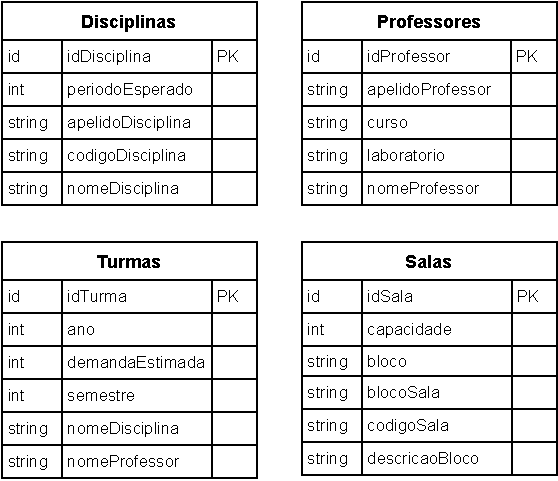
\includegraphics[width=0.7\textwidth]{files/img/2.02!5-desenvolvimento/2.02!5.4-sistema/5.4.2-MVP2/Diagrama_ER-As_is}
\end{MyCenteredFigure}

\paragraph*{B2) Acesso ao Banco de Dados}

Seguindo a mesma sequência de camadas, o acesso ao banco de dados continua sendo feito através de requisições HTTP, porém, ao invés de serem enviadas ao JSONBin, são enviadas a um servidor local que executa as operações no banco de dados. Essa modificação é representada pela seção inferior da \autoref{fig:API_MVP2}.

No \textit{frontend}, enquanto que para acessar a API já pronta do JSONBin foi utilizado o objeto \textit{XMLHttpRequest}, para a comunicação com o banco de dados local, foi utilizada a biblioteca \LinkToURL{\LinkAxios}{\textit{Axios}} para construir as requisições HTTP. E elas, ao invés de serem enviadas ao JSONBin, são enviadas ao \textbf{servidor local}.

Na criação deste \textbf{servidor local} utilizou-se a biblioteca \LinkToURL{\LinkExpress}{\textit{Express}} para desenvolver um \textit{backend} local executado com o \LinkToURL{\LinkNodeJS}{Node.js} paralelo ao \textit{frontend}. Essa biblioteca é responsável por criar todas as rotas necessárias para a comunicação entre o \textit{frontend} e o banco de dados. A partir disso, foi possível criar rotas para cada uma das entidades, e para cada uma das operações CRUD. Com isso, cada operação CRUD em cada uma das rotas é encaminhada para uma \textbf{função específica} que executa a operação no banco de dados.

Este uso, embora exemplifique a aplicação da permanência dos dados, está limitado por dois aspectos: em primeira instância, a permanência dos dados é limitada ao servidor local, não sendo este o desejo final do sistema. Em segunda instância, para haver o acesso aos dados, é necessário que, além do banco de dados, o \textit{backend} também esteja em execução, entretanto, o GitHub Pages, onde o sistema está hospedado, não viabiliza essa execução. Com isso viu-se necessária a busca por um serviço de hospedagem que disponibilizasse a execução do \textit{backend}.

\subsubsection*{\textbf{Logomarca}} \label{sssec:Logomarca}

Um dia após o Natal, foi criado um dos arquivo do sistema chamado ``hourclassMagic.js'', este arquivo agrupava funções que consistiam basicamente em adicionar e remover horários (\textit{hour}) e turmas (\textit{class}) da listagem de turmas e horários. Porém, considerando que a junção dos nomes \textit{hour} e \textit{class} era consideravelmente similar à palavra \textit{hourglass} (``ampulheta'' em inglês) e que a ampulheta é um símbolo que remete ao tempo, e que o sistema é um sistema de alocação de horários, optou-se por utilizar a ampulheta como símbolo do sistema. Quanto ao nome, como o sistema visa a alocação de turmas, especificamente para o curso de Ciência da Computação na UENF, decidiu-se pela corruptela da palavra \textit{hour} para que se tornasse \textit{our}, que significa ``nosso'' em inglês, assim, remetendo ao sentido de individualidade do sistema. Com isso, o nome do sistema se tornou \textit{OurClass}.

\begin{MyCenteredFigure} \caption{Logomarcas do sistema} \label{fig:Logomarcas}
  
\includegraphics[width=\textwidth]{files/img/2.02!5-desenvolvimento/2.02!5.4-sistema/5.4.2-MVP2/Logomarcas}
\end{MyCenteredFigure}

Juntando o símbolo da ampulheta com o nome \textit{OurClass} e outros elementos gráficos, como as tabelas horárias, foi criada a logomarca do sistema, que pode ser vista na \autoref{fig:Logomarcas}. A logomarca foi criada utilizando de inteligências artificiais generativas, principalmente o \textit{Bing}. A partir disso, foi possível criar uma logomarca que refletisse o propósito do sistema, e que fosse agradável visualmente. Após analisar as possibilidades, foi escolhida a \autoref{fig:logomarca_oficial} como a logomarca oficial do sistema. A logomarca foi então adicionada ao sistema.

\begin{MyCenteredFigure} \caption{Logomarca oficial} \label{fig:logomarca_oficial}
  
\includegraphics[width=0.5\textwidth]{files/img/2.02!5-desenvolvimento/2.02!5.4-sistema/5.4.2-MVP2/OurClass}
\end{MyCenteredFigure}

\subsubsection*{\textbf{Funcionalidades adicionais: conflitos, filtragem e disciplinas não oferecidas}} \label{sssec:Funcionalidades Adicionais}

Acrescendo à visualização de conflitos desenvolvida na primeira versão, foi implementada a visualização de conflito por capacidade de salas, ao comparar com a quantidade de alunos estimados para a turma. Mais detalhes sobre os conflitos podem ser vistos mais adiante na \autoref{sec:conflitos} denominada \nameref{sec:conflitos}.

Adicionou-se também diversas filtragens, principalmente na página de \textbf{Grade Horária}. Dessa forma, torna-se possível a visualização específica de turmas que atendam a certos critérios. Essa filtragem é feita através de caixas de seleção, onde é possível selecionar quais critérios se deseja filtrar, sendo eles: ano, semestre, disciplina, professor, sala e categoria. Nessa última distinguem-se as disciplinas por períodos esperados para uma disciplina do curso de Ciência da Computação, e até mesmo, se são opcionais ou de outros cursos. Essa coletânea de filtros viabiliza uma análise mais limpa das informações estruturadas, podendo então gerar \textit{insights} quanto ao posicionamento histórico das turmas.

Outra utilidade adicionada, agora na página \textbf{MultiTurmas}, foi a seção de ``Disciplinas ainda não oferecidas''. Sua funcionalidade consiste em dispor ao usuário uma lista de disciplinas que, segundo a matriz curricular de Ciência da Computação, deveriam ser ofertadas naquele semestre. A partir disso, o usuário pode então selecionar o botão correspondente àquela disciplina e, a partir disso, uma turma para esta disciplina é adicionada à lista de turmas ofertadas. Há também um botão no topo que permite a adição de todas as disciplinas de uma vez.

\subsection{Versão 3.0} \label{ssec:MVP3}                                               % #### 5.4.3

A primeira versão trouxe a possibilidade de se visualizar o sistema, a segunda trouxe a possibilidade de se manter os dados. A terceira e última versão do sistema foi desenvolvida de forma a estar completamente hospedada na nuvem, incluindo o seu banco de dados. Assim como na versão anterior, alguns novos ajustes foram feitos na definição e distribuição de tarefas no \hyperref[sssec:GitHub Projects]{GitHub Projects}. Mas os dois principais focos desta versão foram o uso da \hyperref[sssec:Amazon Web Services]{Amazon Web Services} para a hospedagem do banco de dados e a \hyperref[sec:Solução inicial]{reimplementação da heurística para criação de uma grade horária inicial}.

\subsubsection*{\textbf{Mudanças no GitHub Projects}} \label{sssec:Mudanças no GitHub Projects}

O uso do GitHub Projects se provou como uma excelente forma de organização das tarefas, e assim, foi mantido para a terceira versão. Alguns novos detalhes foram adicionados em sua organização, como a adição da categorização de tarefas por \textbf{Marcos} (\textit{Milestones}) e \textbf{Etiquetas} (\textit{Labels}).

\begin{MyCenteredFigure} \caption{Marcos concluídos do GitHub Projects} \label{fig:ProjectsClosedMilestones}
  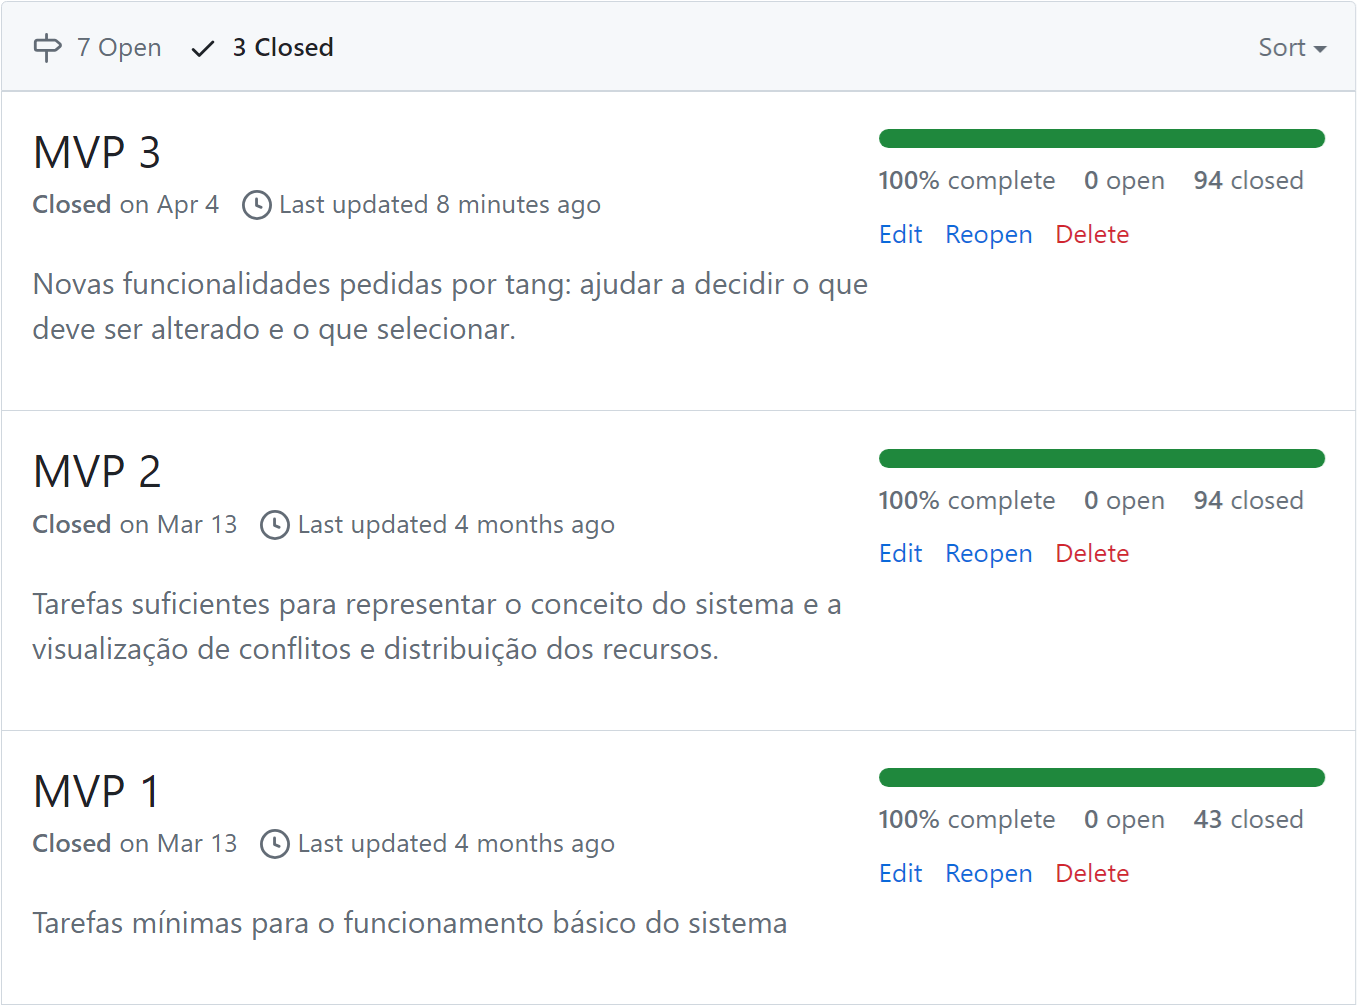
\includegraphics[width=0.9\textwidth]{files/img/2.02!5-desenvolvimento/2.02!5.4-sistema/5.4.3-MVP3/GitHubProjects-Closed_Milestones-Light}
\end{MyCenteredFigure}

\subsubsubsection*{A) Marcos e Etiquetas} \label{ssssec:Marcos e Etiquetas}

Os \textbf{Marcos} visam distinguir as tarefas por suas versões, e também por seus tipos de funcionalidades futuras, assim, a medida em que surgiam novas ideias, elas eram adicionadas ao GitHub Projects. Dessa forma, garantindo uma metrificação do andamento de cada categoria de funcionalidades, além de afunilar a quantidade de tarefas realmente prioritárias para o sistema.

\begin{MyCenteredFigure} \caption{Marcos abertos do GitHub Projects} \label{fig:ProjectsOpenMilestones}
  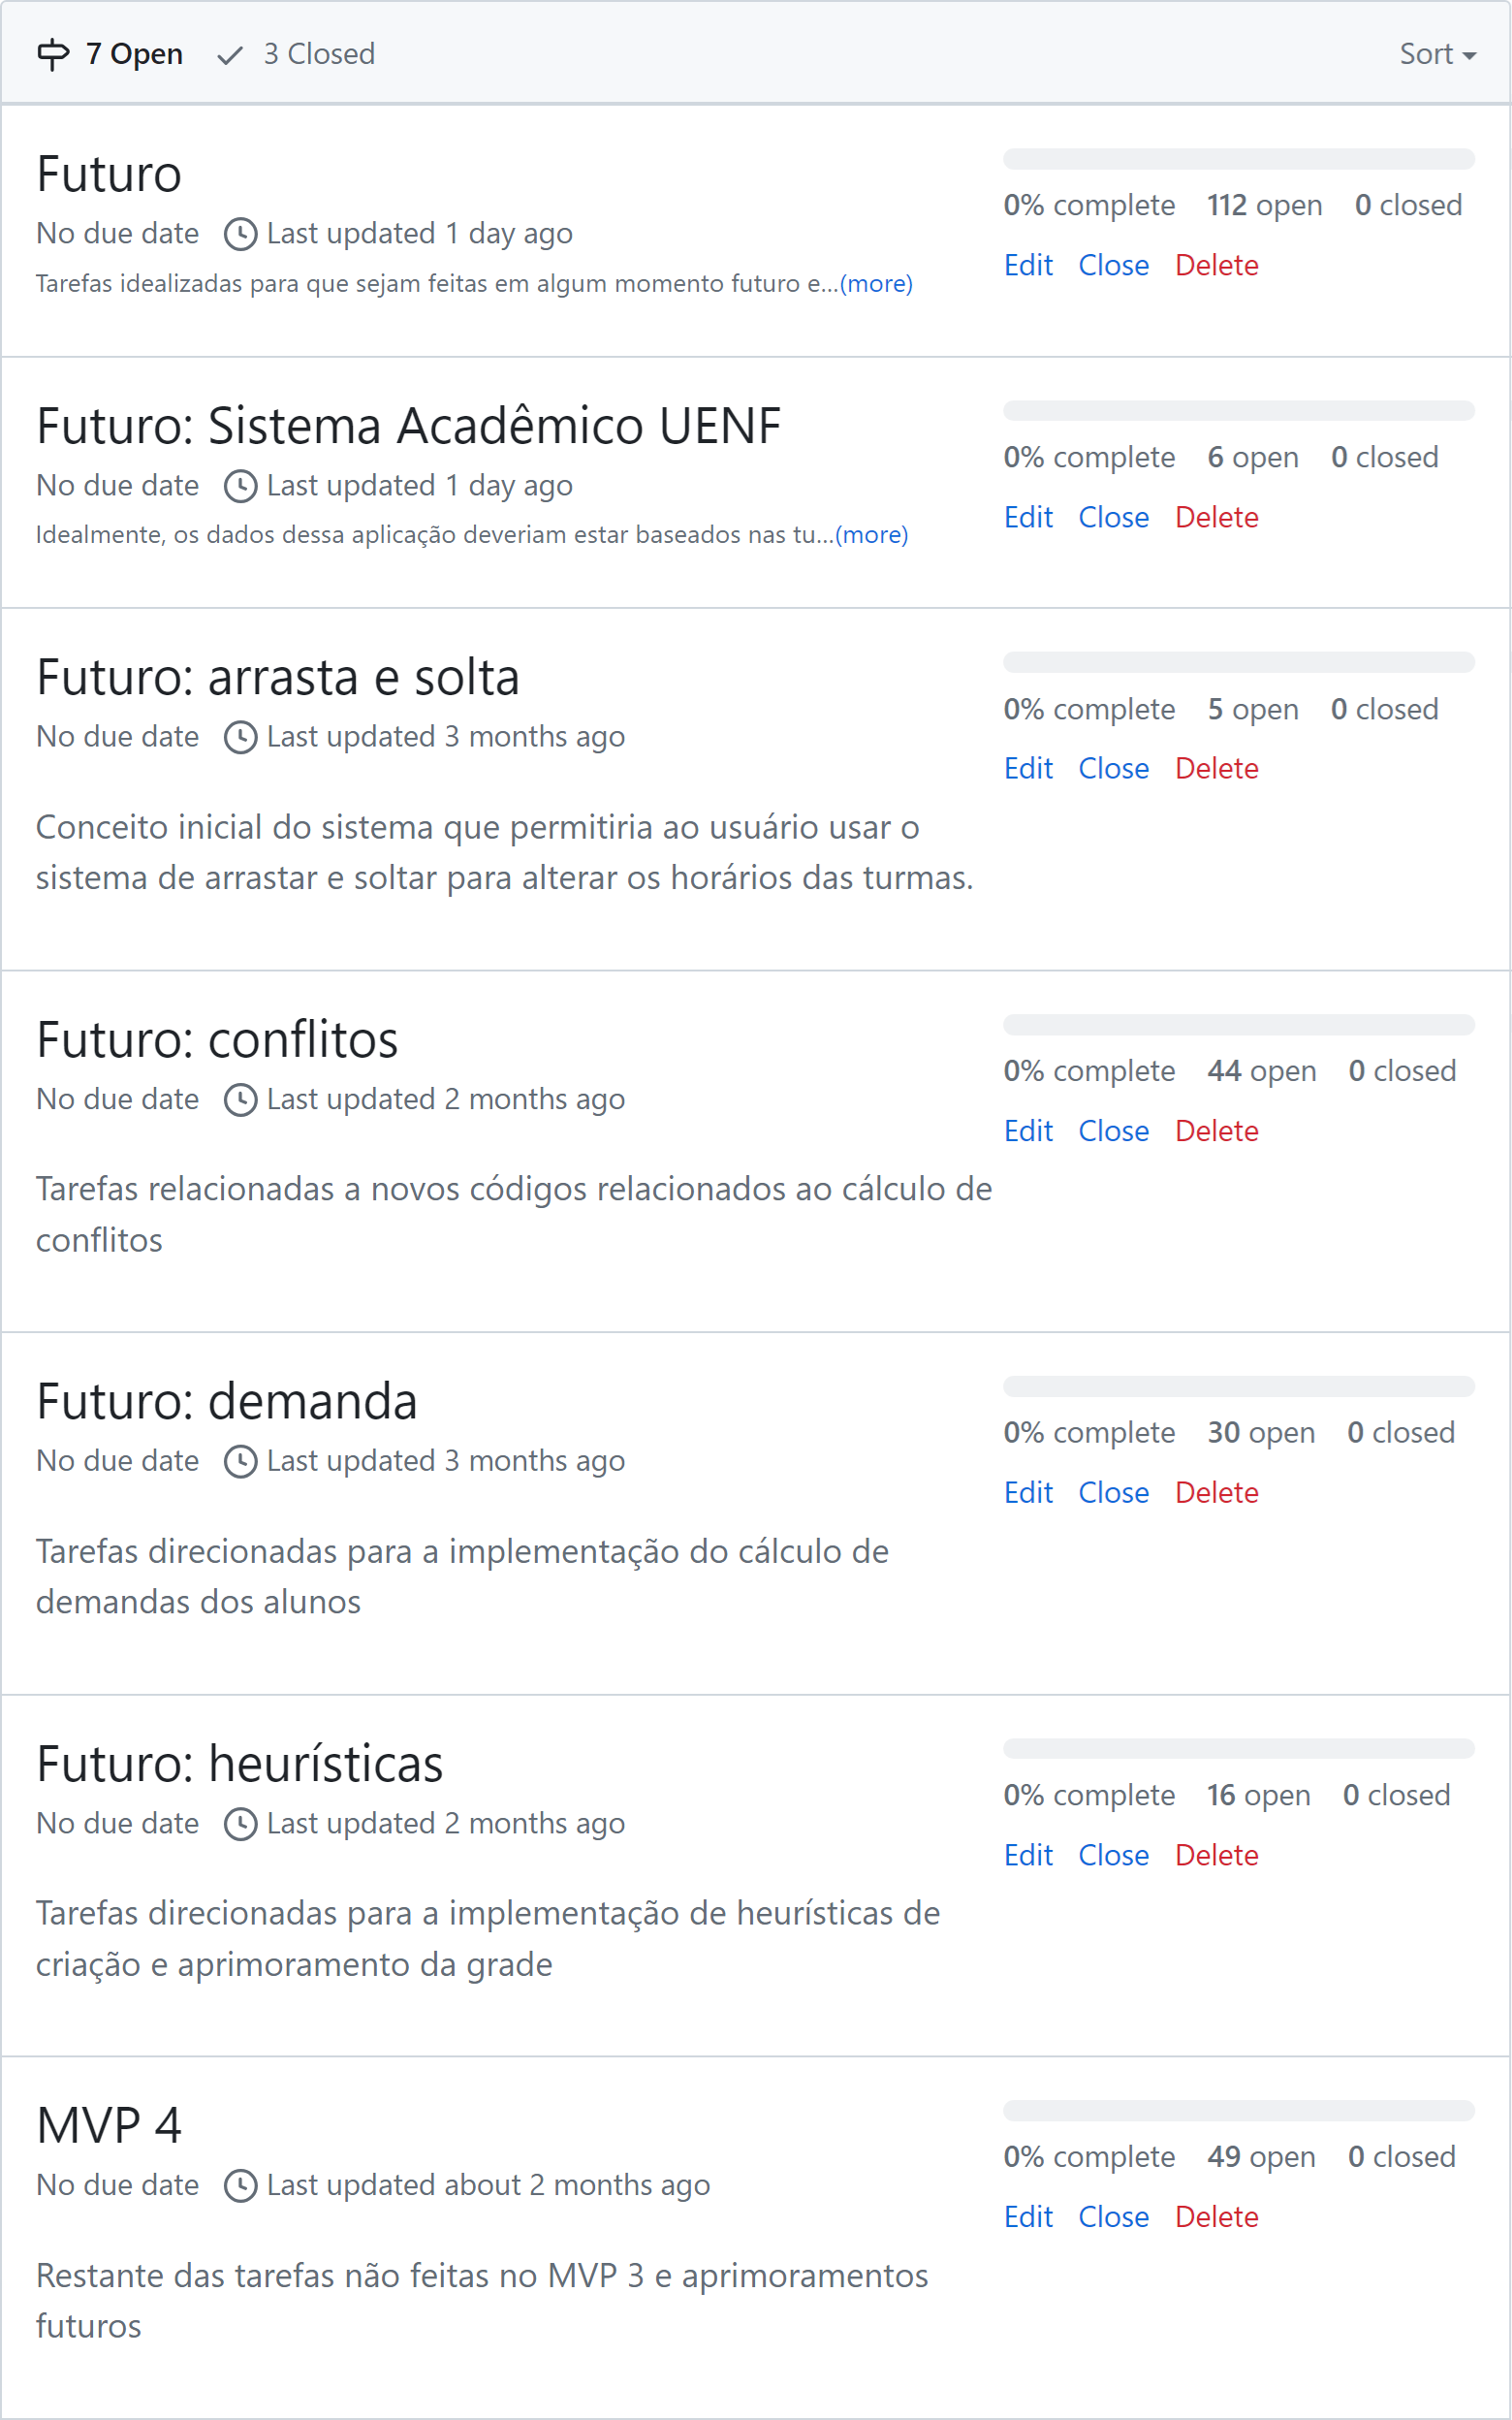
\includegraphics[width=0.9\textwidth]{files/img/2.02!5-desenvolvimento/2.02!5.4-sistema/5.4.3-MVP3/GitHubProjects-Open_Milestones-Light}
\end{MyCenteredFigure}

A \autoref{fig:ProjectsClosedMilestones} mostra os marcos que já foram concluídos, sendo eles as três versões desenvolvidas, e a \autoref{fig:ProjectsOpenMilestones} mostra os marcos que ainda estão em aberto, podendo ser retomadas no futuro.

\begin{itemize}
  \item Marcos Abertos
        \begin{enumerate}
          \item \textbf{MVP 1}: foram concluídas na primeira versão;
          \item \textbf{MVP 2}: foram concluídas na segunda versão;
          \item \textbf{MVP 3}: foram concluídas na terceira versão;
        \end{enumerate}
  \item Marcos Fechados
        \begin{enumerate}
          \item \textbf{MVP 4}: planejadas para a próxima versão a ser desenvolvida;
          \item \textbf{Futuro}: foram planejadas para o futuro do sistema;
          \item \textbf{Heurísticas}: visam aprimorar a alocação de turmas através de heurísticas;
          \item \textbf{Conflitos}: visam aprimorar a visualização, qualidade e/ou variedade de conflitos;
          \item \textbf{Integração com o Sistema Acadêmico UENF}: visam a integração do atual sistema com o sistema acadêmico da UENF.
          \item \textbf{Arrasta e solta}: visam aprimorar a alocação de turmas através de um sistema de arrastar e soltar;
          \item \textbf{Demandas}: visam calcular a demanda dos alunos por disciplinas;
        \end{enumerate}
\end{itemize}

No GitHub Projects, também foram adicionadas as \textbf{etiquetas} (\autoref{fig:ProjectsLabels}) que distinguem as tarefas por seu intuito. As etiquetas utilizadas foram as seguintes:

\begin{MyCenteredFigure} \caption{Etiquetas do GitHub Projects} \label{fig:ProjectsLabels}
  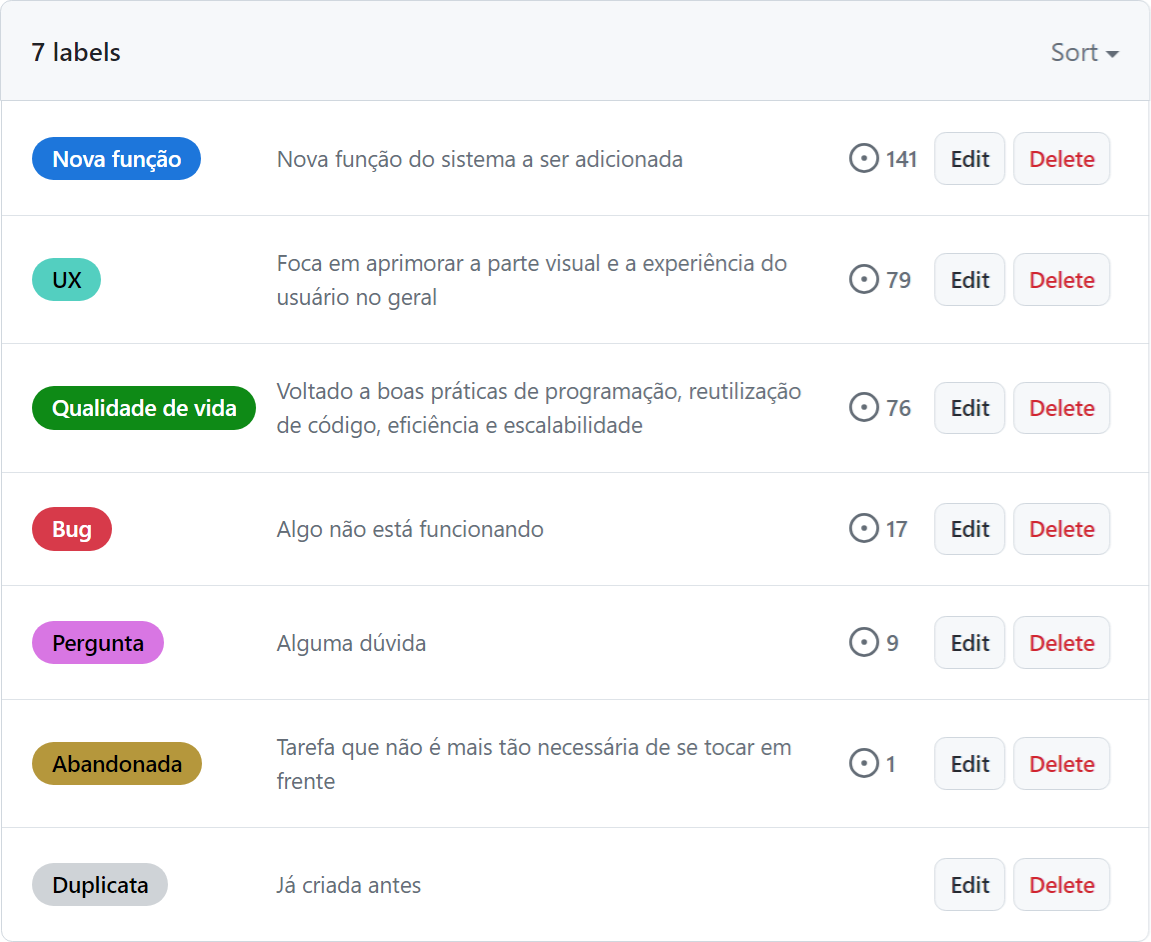
\includegraphics[width=0.7\textwidth]{files/img/2.02!5-desenvolvimento/2.02!5.4-sistema/5.4.3-MVP3/GitHubProjects-Labels-Light}
\end{MyCenteredFigure}

\begin{enumerate}
  \item \textbf{Nova função}: funcionalidades que ainda não foram implementadas;
  \item \textbf{Qualidade de vida}: melhorias que não são necessárias, mas que aprimoram o processo de desenvolvimento;
  \item \textbf{UX}: aprimoramento da experiência do usuário;
  \item \textbf{Bug}: correção de bugs;
  \item \textbf{Pergunta}: dúvidas sobre a validade da tarefa;
  \item \textbf{Abandonada}: quando criada parecia interessante, mas que se decidiu por não implementar;
  \item \textbf{Duplicata}: já foi criada antes e que foi descartada;
\end{enumerate}

\subsubsubsection*{B) Gráficos} \label{ssssec:Gráficos}

O GitHub Projects também oferece a possibilidade de visualização de gráficos na seção \textit{Insights}, que mostram a quantidade de tarefas em cada uma das categorias. Esses gráficos são úteis para a visualização do andamento do projeto, e para a identificação de possíveis gargalos. Com eles, pode-se ter uma noção das métricas do projeto, como por exemplo:

\begin{MyCenteredFigure} \caption{Gráfico de Marco \textit{versus} quantidade de tarefas separadas por etiqueta} \label{fig:ProjectsInsights}
  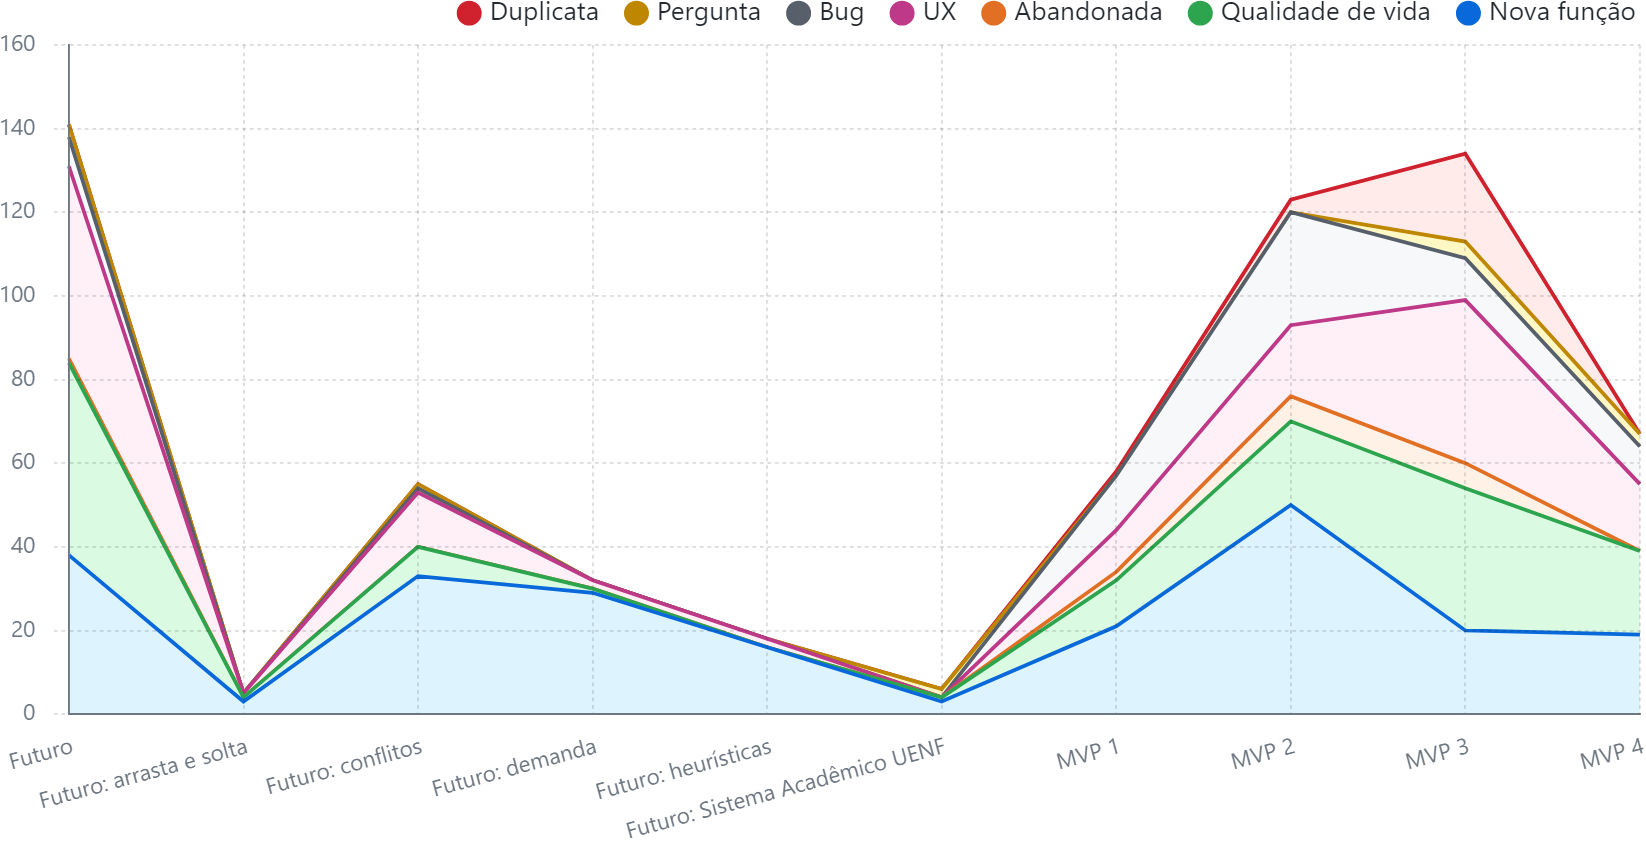
\includegraphics[width=\textwidth]{files/img/2.02!5-desenvolvimento/2.02!5.4-sistema/5.4.3-MVP3/GitHubProjects-Insights-Stacked_Line-Milestone_Label-Light}
\end{MyCenteredFigure}

\begin{itemize}
  \item Quantidade de tarefas de determinada etiqueta a cada marco, exemplificado na \autoref{fig:ProjectsInsights};
  \item Quantidade de tarefas por marco;
  \item Quais páginas receberam tarefas de quais etiquetas;
  \item Quantas são as tarefas em cada um de seus estados (\textbf{completa}, \textbf{em progresso} ou \textbf{pendente}).
\end{itemize}

\subsubsection*{\textbf{\textit{Amazon Web Services}}} \label{sssec:Amazon Web Services}

Para suprir a necessidade de um servidor que pudesse executar o \textit{backend} do sistema em conjunto com o banco de dados, foi escolhido a \textit{Amazon Web Services} (AWS). A AWS é um serviço de computação em nuvem que oferece uma ampla gama de serviços, entretanto, apenas alguns deles foram necessários para o sistema.

\begin{MyCenteredFigure} \caption{Diagrama da permanência dos dados na versão 3.0} \label{fig:API_MVP3}
  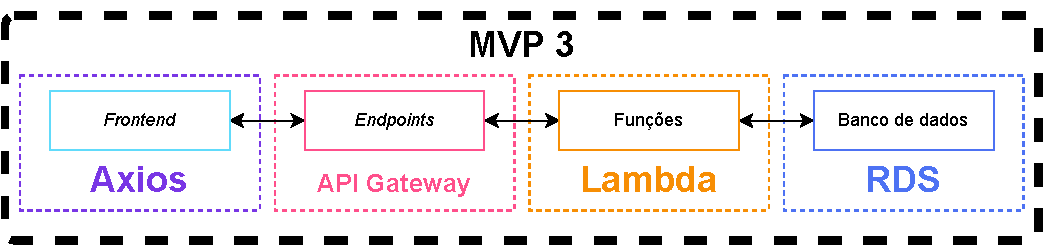
\includegraphics[width=\textwidth]{files/img/2.02!5-desenvolvimento/2.02!5.4-sistema/5.4.3-MVP3/API_MVP3}
\end{MyCenteredFigure}

O uso da AWS segue a mesma lógica do servidor local, com a diferença de que o servidor está em nuvem, e não localmente, assim resolvendo o primeiro dos dois problemas citados. Neste contexto o uso da AWS, representado pela \autoref{fig:APIAWS}, foi feito através de três serviços principais: o \textit{API Gateway} para a recepção das requisições HTTP, o \textit{Lambda} para a execução das funções que acessam o banco de dados, e o \textit{RDS} para o armazenamento dos dados; serviços estes que serão descritos mais detalhadamente a seguir. O uso desses três serviços permitiu a execução do \textit{backend} do sistema em nuvem, e assim, atingindo a permanência dos dados. Com isso, o sistema passou a ser capaz de manter os dados mesmo após a recarga da página, e assim, atender a uma das principais necessidades do sistema.

\begin{MyCenteredFigure} \caption{API REST no AWS} \label{fig:APIAWS}
  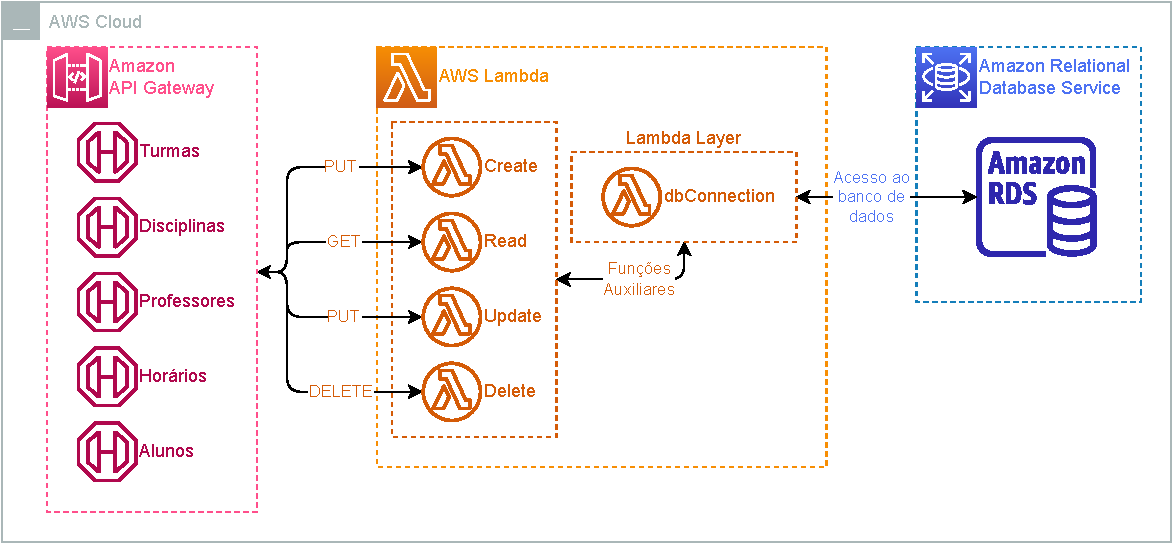
\includegraphics[width=\textwidth]{files/img/2.02!5-desenvolvimento/2.02!5.4-sistema/5.4.3-MVP3/API-Funcionamento}
\end{MyCenteredFigure}

% \subsubsubsection*{A) CORS} % Até agora não entendi direito pra que serve isso. \label{CORS}

\subsubsubsection*{A) Implantação} \label{ssssec:Implantação}

O conjunto de funcionalidades da AWS envolve em grande parte o objetivo de manter um sistema constantemente acessível através da internet, ainda assim, durante o desenvolvimento, ou até mesmo durante o ciclo de vida do software, é esperado que ocorram manutenções periódicas nas quais é compreensível que o sistema fique fora do ar. Sendo assim, para manter-se visando ao máximo a acessibilidade do sistema, espera-se que o mesmo fique desconectado o mínimo possível.

Tanto o API Gateway quanto as funções Lambda precisaram sofrer diversas modificações ao longo do desenvolvimento. A aplicação dessas modificações é chamada de implantação (\textit{deploy}), onde a AWS substitui a versão atual do sistema pela nova versão. Essa aplicação de modificações foi inicialmente feita através da interface \textit{web} da AWS, porém, com o tempo, foi percebido que essa abordagem era ineficiente. No caso das implantações do API Gateway, visto que assim que as rotas estiverem configuradas, não há a necessidade de alterá-las, não havia grande impacto no fluxo de trabalho. Já no caso das funções Lambda, cada mínima mudança no código requisitava um novo \textit{deploy} para cada uma das funções alteradas.

Outro detalhe percebido, foi que boa parte do código se repetia entre as funções que interagiam diretamente com o banco de dados. Sendo assim, passou-se a utilizar das \textit{Lambda Layers}, que são camadas que podem ser compartilhadas entre diversas funções, e assim, diminuir a quantidade de código repetido. Essa nova abordagem permitiu que as funções fossem mais enxutas, e que as mudanças fossem aplicadas de forma mais rápida, visto que bibliotecas e funções comuns entre as funções eram compartilhadas entre elas.

\subsubsubsection*{B) AWS CLI} \label{ssssec:AWS CLI}

Nas primeiras tentativas de \textit{deploy}, duas abordagens eram utilizadas: a primeira era a de copiar e colar o código diretamente na interface web da AWS, e a segunda era a de fazer o upload de um arquivo zip contendo o código.

\lstinputlisting[captionpos={t}, label={code:lambda}, caption={Código de \textit{deploy} de Lambda}]{files/codigos/AWS_CLI.sh}

Como mostrado no \autoref{code:lambda}, usa-se o software AWS CLI para criar uma função lambda. O comando \textit{create-function} é o comando que cria a função, e os argumentos que seguem são os parâmetros necessários para a criação da função. O \textit{function-name} é o nome da função, o \textit{runtime} é a versão do Node.js que a função utiliza, o \textit{role} é o conjunto de permissões criadas na seção \textit{AWS Identity and Access Management} (IAM), o \textit{handler} é o nome do arquivo principal que contém a função, e o \textit{zip-file} é o arquivo zip que contém o código da função.

Com isso, ao executar o comando, a função é criada, e então, a nova versão do código é aplicada. Com este fluxo de trabalho, embora permita o \textit{deploy} sem a direta conexão ao sistema AWS, ainda assim é necessário executar comandos específicos para cada uma, tendo que manualmente compactar o código e fazer o upload de cada um dos arquivos das diversas funções coexistentes.

\subsubsubsection*{C) SAM} \label{ssssec:SAM}

Como solução, foi utilizado o AWS SAM (\textit{Serverless Application Model}), que é uma extensão do \textit{AWS CloudFormation} que simplifica o desenvolvimento de aplicações sem servidor. O AWS SAM permite a definição de aplicações sem servidor de forma mais simples, e a partir disso, é possível fazer o \textit{deploy} de toda a aplicação de uma vez só. O uso do AWS SAM foi feito através de um arquivo \textit{template.yaml}, que contém a definição de todas as funções Lambda, e de recursos necessários para o funcionamento do sistema.

Como mostrado no \autoref{code:template} disposto no \autoref{apendice:ExemploTemplateYAML}, o arquivo \textit{template.yaml} contém a definição de algumas das estruturas utilizadas para este sistema, principalmente as funções Lambda, visto que são quatro funções para cada uma das seis entidades, totalizando 24 funções. O arquivo contém a definição de cada uma das funções, e de cada uma das rotas que elas atendem. A partir disso, é possível fazer o \textit{deploy} de todas as funções que foram alteradas de uma vez só, e assim, diminuir o tempo de \textit{deploy} e a quantidade de comandos necessários.

Após o preparativo do arquivo \textit{template.yaml}, o \textit{deploy} é feito através do conjunto de comandos \textit{sam build; sam deploy}, que primeiro combina o \textit{CloudFormation Template} com o código da aplicação, e em seguida realiza o \textit{deploy} de todas as funções definidas no arquivo. Com isso, o sistema passou a ser mais facilmente atualizável, e mais facilmente mantido.

\subsubsubsection*{D) Outros serviços da AWS} \label{ssssec:Outros serviços da AWS}

Os serviços listados até então foram os principais utilizados para a execução do \textit{backend} do sistema, entretanto, diversos outros serviços foram utilizados para a manutenção do sistema como um todo e para a execução de tarefas secundárias. Abaixo estão listados alguns desses serviços.

\begin{itemize}
  \item \textbf{S3}: serviço de armazenamento de objetos, utilizado para armazenar os objetos gerados pelo CloudFormation;
  \item \textbf{CloudWatch} e \textbf{CloudTrail}: serviço de monitoramento, utilizado para a visualização de métricas do sistema;
  \item \textbf{IAM}: serviço de gerenciamento de permissões, utilizado para a definição de permissões para as funções Lambda;
  \item \textbf{VPC}: serviço de rede privada virtual, utilizado para a definição de uma rede privada para o sistema;
  \item \textbf{Cost Explorer}: serviço de visualização de custos, utilizado para a visualização dos custos do sistema;
\end{itemize}

\subsubsection*{\textbf{Melhorias no sistema}} \label{sssec:Melhorias no Sistema}

O sistema passou por diversas pequenas mudanças, e algumas maiores. Uma considerável parte delas foi relacionada à forma com que as informações eram estruturadas internamente, mudanças essas feitas com o intuito de tornar o sistema mais fácil de ser mantido posteriormente. Em seguida estão listadas algumas das várias melhorias feitas no sistema.

\subsubsubsection*{A) Filtros e ordenações} \label{ssssec:Filtros e ordenações}

Levando em consideração a multidimensionalidade da estrutura dos dados, a possibilidade de realizar ``curvas de nível'' e as ordenar por diferentes critérios se mostrou uma funcionalidade essencial para a compreensão dos dados. Dessa forma, em diferentes páginas do sistema, foram adicionadas ordenações padrões e seletores de filtragem manual, assim permitindo ao usuário a visualização de dados específicos.

Alguns exemplos de casos de uso dessas funcionalidades seria: ``Na página \textbf{MultiTurmas} o Professor A está tendo conflitos em suas turmas, então o usuário pode filtrar as turmas do Professor A e visualizar apenas as suas turmas. Em seguida, o usuário percebe que o Professor A está em conflito com a Sala B123, então o usuário visualiza apenas as turmas da Sala B123. Por fim, o usuário encontra um outro horário disponível para o Professor A e a Sala B123, e então, o conflito é resolvido.''

Uma das solicitações presentes ao final da versão anterior foi quanto a uma distinção mais clara entre disciplinas de Ciência da Computação e disciplinas de outros cursos. Para isso, embora não pareça apresentar grande robustez na forma como foi feito, apresenta suficiente clareza para o usuário final. A distinção foi feita ao utilizar o campo \textbf{Período Esperado} presente na entidade \textbf{Disciplina}, para definir que:

\begin{itemize}
  \item \textbf{1 $\leq$ Período Esperado $\leq$ 10}: Disciplina obrigatória de Ciência da Computação;
  \item \textbf{Período Esperado = 11}: Disciplina eletiva optativa para Ciência da Computação;
  \item \textbf{Período Esperado = 12}: Disciplina eletiva livre para Ciência da Computação;
  \item \textbf{Período Esperado = 13}: Disciplina não ofertada para Ciência da Computação;
\end{itemize}

Com essa divisão, definiu-se o sistema para que, por padrão, apenas exibisse as turmas voltadas para Ciência da Computação, e que, caso o usuário desejasse, poderia visualizar as turmas de outros cursos.

\subsubsubsection*{B) MultiTurmas} \label{ssssec:MultiTurmas}

Dentre as tarefas realizadas, uma das páginas que mais sofreu alterações foi a página de \textbf{MultiTurmas}. Nela, foram feitas diversas melhorias, como a adição de filtros, ordenações e aprimoramento dos textos contidos nas caixas de seleção.

\paragraph*{B1) Adição da propriedade ``descrição''} \label{par:Descrição}

Disciplinas oferecidas em um mesmo semestre por vezes são oferecidas para alunos demais para que uma única turma os comporte, e assim, é necessário a criação de mais de uma turma. Para que os alunos e professores possam identificar facilmente a qual turma pertencem, foi adicionada a propriedade descrição, que é uma breve descrição da turma. Esse código descritor já se encontra no Sistema Acadêmico, porém com a limitação de apenas 3 caracteres. No presente trabalho, a descrição pode conter até 255 caracteres.

Adicionando esse campo, a visualização linear das informações da turma se tornou mais difícil de apresentar na tela. Considerando que em sua maioria as turmas possuem dois horários, dispôs-se então as informações em conjuntos de dois elementos, ao invés de uma lista única, tornando então a visualização mais densa.

\paragraph*{B2) Aprimoramento dos identificadores dos conflitos}

Os conflitos ocorridos indicavam quais eram os identificadores (ids) das turmas que estavam em conflito, porém, esses ids eram referentes ao banco de dados, sendo ele um valor numérico, não continha valor semântico suficiente para ser facilmente identificado. Estes ids eram visualizados ao posicionar o ponteiro do mouse por sobre os componentes cujo conflito foi verificado. Com isso, foi feita a adição de um novo identificador, que é composto pelas informações contidas na turma, sendo elas o ano, semestre, nome da disciplina, nome do professor, e o código descritor da turma. A partir disso, tornou-se mais fácil identificar quais turmas estavam em conflito, e assim, corrigi-las. Essa identificação foi adicionada também aos horários, onde o identificador passou a ser composto pela sala, dia da semana, horário de início e fim.

\paragraph*{B3) Criação e deleção de turmas e horários}

Embora seja uma funcionalidade básica e existente desde a primeira versão, a criação e deleção de turmas apresentou diversos problemas ao longo do desenvolvimento. Um dos mais cruciais era devido à assincronicidade intrínseca ao uso de um banco de dados remoto. O problema era que durante a criação sequencial de duas turmas, apenas a segunda era mostrada, mesmo que ambas tivessem sido criadas.

O que ocorria era que, ao começar com a lista de $Turmas = [A, B]$ tenta-se adicionar a turma $C$ à lista de $Turmas$, mas para isso, a requisição enviada ao banco de dados deve retornar com o status de sucesso, e para que, só assim, fosse adicionada à listagem apresentada no sistema. Então, caso fosse feita a tentativa de se adicionar a turma $D$ antes da confirmação anterior ser recebida, a adição seria realizada novamente na listagem inicial ($[A, B]$). Por fim, assim que a primeira requisição retornasse bem sucedida, por um breve instante a listagem seria $[A, B, C]$, e então, após a adição da turma $D$, a listagem seria $[A, B, D]$. Para resolver esse problema, foi feita a adição de uma função de \textit{callback} que passou a utilizar o estado mais atual da listagem de turmas, e não mais a listagem inicial.

Outra característica aprimorada, foi a velocidade de adição e deleção, principalmente a de deleção. Antes, a aprovação do banco de dados era necessária para que a lista de turmas fosse atualizada, e isso tornava o processo de deleção lento. Para resolver isso, foi feita a adição de uma função de deleção que remove a turma da listagem de turmas antes mesmo da confirmação do banco de dados. Essa não se mostra como a solução mais adequada, visto que em caso de falha na deleção, a turma poderá ser restaurada com a simples atualização da página, os pontos positivos na usabilidade superam os negativos.

\paragraph*{B4) Aprimoramento das disciplinas não oferecidas} \label{par:Solução inicial}

A funcionalidade \hyperref[sssec:Funcionalidades Adicionais]{anteriormente denominada ``Disciplinas ainda não oferecidas''} foi aprimorada de tal forma que agora, além de criar uma turma para a disciplina selecionada, o sistema automaticamente analisa o histórico de criação de turmas, definindo previamente o professor, a demanda estimada, e os horários, incluindo seus dias, horas de início e sala em que é alocada. Então, após a criação de todas as turmas referentes ao curso de Ciência da Computação, uma solução inicial foi obtida. Sendo ela mais detalhadamente descrita posteriormente na \autoref{sec:Solução inicial} denominada \nameref{sec:Solução inicial}.

\subsubsubsection*{C) Grade horária} \label{ssssec:Grade Horária}

A página que detinha o nome ``CCTable'' e que visava apresentar exclusivamente as disciplinas do curso de Ciência da Computação, foi renomeada para ``Grade Horária'', e passou a ser possível de apresentar disciplinas de todos os cursos, embora ainda não seja possível distinguir as disciplinas de um curso para o outro. As células das turmas sofreram um ligeiro aprimoramento visual e foram ordenadas primariamente por seu período esperado.

\subsubsubsection*{D) Banco de dados} \label{ssssec:Banco de dados}

Quanto ao banco de dados, os dados antes desconexos passaram a ser interligados adequadamente por chaves estrangeiras. Apresentando então restrições em casos de deleções inapropriadas no banco de dados. A API, por sua vez, deixou de retornar as listas de turmas, professores, disciplinas e salas, e passou a retornar os dados de forma mais estruturada em formato JSON.

\begin{MyCenteredFigure} \caption{Novo diagrama de banco de dados} \label{fig:MVP3_BancoDeDados}
  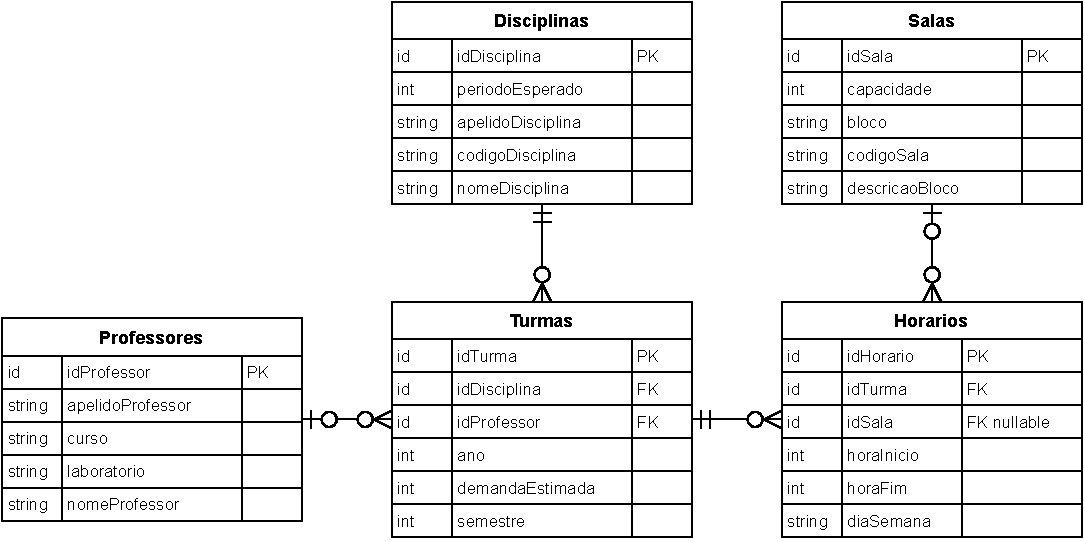
\includegraphics[width=\textwidth]{files/img/2.02!5-desenvolvimento/2.02!5.4-sistema/5.4.3-MVP3/Diagrama_ER-How_it_should_be}
\end{MyCenteredFigure}

Na \autoref{fig:MVP3_BancoDeDados} vemos as inter-relação entre as propriedades das entidades do banco de dados. Com o uso mais apropriado das chaves estrangeiras, o anterior uso dos nomes das disciplinas e professores como elementos de identificação foi substituído pelo uso de seus respectivos códigos identificadores. Houve também o surgimento da entidade \textbf{Horarios}, que interliga as turmas às salas.

\subsubsubsection*{E) Aprimoramento na forma de criação de itens}

Antes, ao acessar a página de criação de entidades, uma entidade era previamente selecionada. E para a criação de uma nova entidade, os valores da entidade anterior deveriam ser alterados, e, ao clicar em adicionar, esses valores alterados eram cadastrados no banco de dados. Essa sequência de ações não apresentou intuitividade suficiente e, portanto, foi alterada. A versão atual passou a não selecionar previamente a entidade. Assim, ao clicar em adicionar um novo item, uma nova entidade é criada. No caso das turmas, a entidade é criada com os valores de ano e semestre predefinidos baseado na filtragem selecionada.

\subsubsubsection*{F) Boas práticas}

Além das funcionalidades voltadas para o usuário final, algumas mudanças classificadas como \textbf{Qualidade de vida} foram realizadas visando a manutenção do sistema. Dentre elas estão:

\begin{itemize}
  \item \textbf{Repadronização de componentes}: como o conhecimento relacionado a boas práticas de programação foi adquirido ao longo do desenvolvimento, partes de componentes criados anteriormente foram reformulados para que estivessem estruturados de acordo com a estrutura recentemente desenvolvida no código.
  \item \textbf{Externalização de informações}: algumas informações constantes como cores de fundo e textos foram externalizadas para variáveis, assim, caso haja a necessidade de alteração, não será necessário a busca manual por todas as ocorrências. Um outro caso desses é referente aos textos dispostos nas caixas de seleção, que foram convertidos em funções que retornam o texto desejado.
  \item \textbf{Inglês}: como as linguagens de programação de modo geral se apresentam no idioma inglês, é considerado uma boa prática que as variáveis e funções também, o que não foi a abordagem inicialmente tomada. Assim, foi feita uma gradual migração para o inglês, e embora não tenha sido concluída, a maior parte do código já se encontra em inglês. Para facilitar essa migração, foi elaborado um sistema de ``\textit{getters}'' como forma de obter a propriedade de determinado objeto, independente de qual língua ele esteja.
  \item \textbf{Remoção de estruturas obsoletas}: ao longo do desenvolvimento, algumas estruturas foram criadas e não utilizadas. Um exemplo dessas foi a propriedade ``Ordem'' que visava definir a ordem em que os horários da turma apareceriam, porém o resultado desta propriedade foi obtido com a ordenação dos horários por dia e em seguida por horário, não sendo então necessária. Ela então foi removida do sistema e do banco de dados.
\end{itemize}

\section{Solução inicial} \label{sec:Solução inicial}                                   % ###  5.5 

Um dos processos mais importantes para a alocação de turmas é a definição de uma solução inicial. Ao longo das versões, a solução inicial foi sendo aprimorada, deixando de \hyperref[sssec:Funcionalidades Adicionais]{criar turmas para todas as disciplinas disponíveis, porém sem as suas informações preenchidas}, para \hyperref[par:Solução inicial]{criar turmas com suas características já preenchidas seguindo uma heurística baseada no histórico de criação de turmas}.

O botão de adição de todas as disciplinas foi mantido, e agora, ao ser clicado, cria as turmas com suas características já preenchidas, assim gerando uma solução inicial, porém passível de conflitos. Vale ressaltar que o preenchimento das características, entretanto, não inclui a propriedade \hyperref[par:Descrição]{descrição}, visto que esta é uma característica única de cada turma e deve ser adicionada manualmente somente em caso de necessidade.

\subsection{Heurística histórica para criação de uma solução inicial} \label{ssec:Heurística}

A solução inicial é obtida através de uma heurística própria que analisa o histórico de criação de turmas com o objetivo de criar todas as turmas necessárias para o semestre. O histórico em que se baseia consiste em todas as turmas, de todos os anos, cadastradas no sistema, sendo elas do curso de Ciência da Computação ou não. A partir disso, define as características das turmas a serem criadas. A heurística é executada assim que o botão de adição de turmas a partir das disciplinas ainda não ofertadas for clicado.

Baseado na grade curricular de 2015, foram armazenadas no sistema as disciplinas e seus respectivos períodos esperados. Com essa informação, é possível distinguir entre disciplinas geralmente oferecidas no primeiro semestre (aquelas cujo período esperado é um número ímpar), e as disciplinas oferecidas no segundo semestre (aquelas cujo período esperado é um número par).

Na seção inferior da página Multiturmas há uma tabela com a listagem das disciplinas esperadas a serem oferecidas no semestre selecionado nos filtros, desde que ainda não tenham sido atreladas a alguma turma naquele semestre. Listagem essa que apresenta as disciplinas pares, ímpares, ou todas, caso o semestre de verão seja selecionado.

Com essas informações o usuário pode escolher criar uma turma para uma \textbf{disciplina em específico}, ou então uma turma para \textbf{cada uma das disciplinas listadas}. Ao criar uma turma para uma \textbf{disciplina específica}, ele inserirá essa disciplina em uma lista de turmas a serem criadas. Já ao criar uma turma para \textbf{todas as disciplinas listadas}, o sistema irá inserir todas as disciplinas da listagem em uma lista de turmas a serem criadas.

A partir daí o sistema percorrerá cada uma das disciplinas na listagem das turmas a serem criadas e, filtrará do cadastro histórico de turmas para que sejam obtidas \textbf{apenas as turmas da disciplina em questão}. Em seguida, a heurística analisa a listagem das turmas já filtradas e define as características das turmas a serem criadas.

O algoritmo de aquisição das informações para a criação da turma é ilustrado no \autoref{code:heuristica} e consiste em 4 funções principais: \textit{splitClasses}, \textit{getMostFrequentClassTimeSizes}, \textit{getMeanDemand} e \textit{getMostFrequent}.

\begin{lstlisting}[language=JavaScript, caption={Heurística de solução inicial}, label={code:heuristica}]
function getUsualInfo(classes) {
  const classTimes = splitClasses(classes);
  const quantity = getMostFrequentClassTimeSizes(classes);
  const classUsualInfo = {
    professor: getMostFrequent(classes, ["professor"]),
    expectedDemand: getMeanDemand(classes),
    // description: getDescription(classes, currentSemester),
    description: null,
    classTime: {
      quantity,
      day: getMostFrequent(classTimes, ["dia"], quantity),
      room: getMostFrequent(classTimes, ["sala"]),
      duration: getMostFrequent(classTimes, ["duracao"]),
      startHour: getMostFrequent(classTimes, ["horaInicio"]),
    },
  };
  return classUsualInfo;
}
\end{lstlisting}

Na função \textbf{\textit{splitClasses}} uma lista de objetos ``turma'' contendo múltiplos horários é passada por parâmetro e é dividido em uma lista de objetos ``turma'', onde cada objeto contém as informações de um dos horários, então retornando uma lista de objetos ``horário''. Essa função realiza esta conversão para que se possa trabalhar com os dados referentes a cada horário de forma individual.

Na função \textbf{\textit{getMostFrequentClassTimeSizes}} é passada uma lista de objetos ``turma'' contendo múltiplos horários e é retornado um número inteiro que representa a quantidade de horários que foi mais frequente dentre as turmas passadas por parâmetro. Essa função é utilizada para definir a quantidade de horários que a nova turma terá.

Na função \textbf{\textit{getMeanDemand}} é passada uma lista de objetos ``turma'' e é retornado um número inteiro que representa a média da demanda de todas as turmas que possuam demanda estimada.

Na função \textbf{\textit{getMostFrequent}} são passados três parâmetros usualmente: uma \textbf{lista de objetos} ``turma'' ou uma lista de objetos ``horário'', uma lista de strings que representam \textbf{o campo que se deseja analisar}, e um número inteiro que representa a \textbf{quantidade de valores} que se deseja retornar, sendo este valor igual a 1 caso nenhum valor seja passado. A função então usa a lista de objetos passada por parâmetro para contar a frequência de cada valor registrado no campo desejado, e então, retorna os valores mais frequentes.

Com essas quatro funções são coletadas as informações pertinentes à turma de tal disciplina, sendo elas: professor, demanda estimada, quantidade de horários, dia, sala, duração e hora de início. E, com esses dados, o sistema criará uma turma para a disciplina em questão contendo as informações obtidas.

\subsection{Requisitos, benefícios e limitações da heurística histórica} \label{ssec:limitacoes_heuristicas}

Como a heurística é baseada no histórico de criação de turmas, é necessário, claro, que haja um histórico de criação de turmas para que a solução inicial seja obtida. E, quanto maior o histórico, mais precisa será a solução inicial obtida.

A heurística é capaz de prever com certa precisão as características das turmas a serem criadas. Entretanto, a solução encontrada está passível de apresentar conflitos visto que nem todas as alocações de turmas apresentam um padrão objetivo. Além disso, a heurística não checa se a turma a ser criada está alocada em um horário já ocupado pelo professor ou sala em questão. Outra limitação é quanto a professores que já não estejam mais associados à instituição ou que acabaram de ser contratados, nesses casos, os mesmos, devido à baixa frequência de alocações, terão menor probabilidade de serem alocados.

Como o usuário tem a capacidade de escolher alocações de apenas algumas disciplinas específicas, a geração da solução inicial pode ser feita parcialmente, o que traz maior flexiblidade ao usuário.

As limitações da heurística encarregam então ao usuário a verificação e a correção dos possíveis conflitos gerados durante a criação da solução inicial. Essa correção se dá através da análise do sistema de \hyperref[sec:conflitos]{detecção e alerta dos conflitos}.

\section{Detecção e alerta dos conflitos} \label{sec:conflitos}                         % ###  5.6

Uma das principais funcionalidades do sistema é a detecção de conflitos. Seu objetivo é auxiliar ao usuário a identificar possíveis problemas na alocação das turmas, e assim, permitir que ele possa corrigi-los antes de finalizar a grade horária. Diversas situações podem ser consideradas como conflitos, e cada uma delas é tratada de forma diferente.

Os conflitos aqui se colocam como uma forma de alerta ao usuário, e não como uma restrição, assim viabilizando ao usuário que uma ação seja tomada, ou não, a partir do alerta. O conceito da não restrição é importante, visto que embora idealmente espera-se que o processo de alocação disponha de todas as informações para que seja otimamente alocado, na prática, isso atualmente não se mostra uma realidade.

Essa flexibilização das restrições que poderiam ser tidas como rígidas em um problema de otimização, é uma característica do problema de alocação de turmas da UENF. Como na realidade da instituição as grades precisam ser criadas enquanto ainda se tem informações incompletas, certas decisões precisam ser tomadas manualmente, sendo então necessária esta flexibilidade para permitir que o usuário possa tomar essas decisões.

Além disso, diversos casos atípicos acabam por ocorrer na realidade da universidade, e que, embora possam não ser aconselháveis ou até mesmo tidos como conflituosos pelo sistema, não seriam de fato um problema para a execução prática das alocações.

\subsection{Conflitos atípicos}

Nessa seção são descritos alguns exemplos de conflitos que poderiam ser alertadas pelo sistema, mas que não seriam realmente um restritor para a execução prática das alocações.

Considerando o corpo docente do curso de Ciência da Computação, que atualmente conta com seis professores doutores, é recorrente a solicitação de professores bolsistas para ministrar disciplinas. Devido aos prazos existentes ao longo do processo de criação da grade horária, é comum que ainda não se saibam quais e quantos professores bolsistas serão disponibilizados para quais turmas. Porém, como o Sistema Acadêmico requere a inserção de professores para a criação de turmas, uma solução encontrada foi a inserção de um desses professores permanentes como responsável pela turma. E, mesmo após se obter a informação quanto a quais e quantos bolsistas estarão disponíveis, ainda assim o sistema acadêmico não os permite serem inseridos, visto que eles não têm um vínculo permanente com a instituição. Com isso, seria possível ver, por exemplo, um conflito entre duas turmas que possuem o mesmo professor em um mesmo horário, mas que na prática, uma delas será ministrada por um professor bolsista.

Outras situações que podem ocorrer giram em torno da alocação das salas. Duas situações que podem ilustrar sua atipicidade são: a possibilidade de alocar uma turma a uma determinada sala, mesmo que se tenha a intenção de ministrá-la em outra, e também a possibilidade de se repartir a turma em duas salas de aula ocorrendo simultaneamente.

\subsection{Conflitos tratados pelo sistema} \label{ssec:ConflitosTratados}

Para a implementação, primeiro visou-se a detecção de conflitos que poderiam ser considerados restritores para a alocação das turmas. Sendo eles os de alocação simultânea de salas e professores, visto que um professor não pode ministrar em duas turmas simultaneamente, nem uma sala deve comportar duas turmas simultaneamente (embora ambos sejam teoricamente possíveis). Além disso, também foi implementada a detecção de conflitos de capacidade, onde a quantidade de alunos de uma turma é maior do que a capacidade da sala alocada, e alguns outros indicativos visuais que serão descritos abaixo.

Os conflitos calculados são representados de três formas diferentes. A primeira e mais perceptível é a mudança de cor de fundo dos atributos conflituosos. A segunda, visando evitar sobreposição de conflitos, é a adição de uma borda inferior que se estende por toda a largura do atributo. E a terceira, mais descritiva, é o uso do atributo \textit{title} dos elementos HTML, que exibe uma mensagem de alerta flutuante ao passar o mouse sobre o atributo conflituoso, assim dispondo de mais detalhes sobre os conflitos buscados e encontrados.

Embora o sistema seja projetado para ser permissivo quanto a inexistência de certas informações, é sempre esperado que a maior quantidade de informações possíveis seja inserida, assim, caso algum campo não tenha sido preenchido a cor de fundo do elemento será alterada para um tom acinzentado.

\begin{MyCenteredFigure} \caption{Paleta de cores do sistema} \label{fig:conflitoDisciplinaPaleta}
  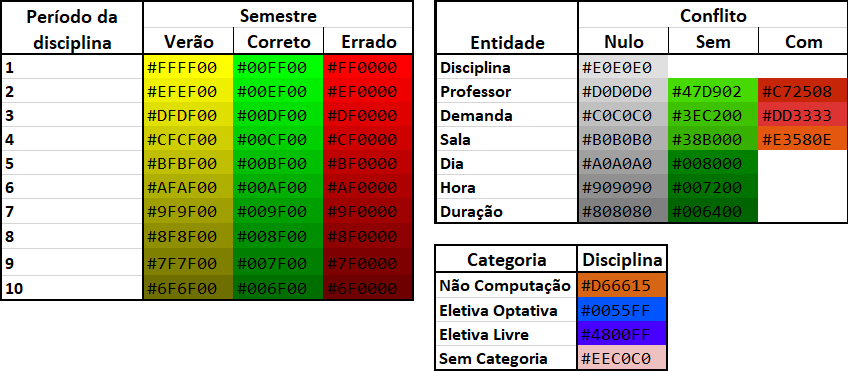
\includegraphics[width=\textwidth]{files/img/2.02!5-desenvolvimento/2.02!5.6-conflitos/Paleta de Cores}
\end{MyCenteredFigure}

Os conflitos que são representados por cores, têm sua paleta de cores representada na \autoref{fig:conflitoDisciplinaPaleta}. Nessa paleta, dispõe-se 3 conjuntos principais: a distribuição de cores para as disciplinas obrigatórias do curso de Ciência da Computação, que variam de acordo com o semestre em que são ofertadas; a categoria das disciplinas não obrigatórias para o curso de Ciência da Computação; e os conflitos das outras entidades, que são classificados amplamente entre ``com conflito'', ``sem conflito'' e ``conflito nulo'' (dados faltantes).

Cinco campos se encontram sem cores, sendo eles a \textbf{Disciplina sem conflito}, \textbf{Disciplina com conflito}, \textbf{Dia com conflito}, \textbf{Hora com conflito} e \textbf{Duração com conflito}. No caso dois dois primeiros, melhor explicado \hyperref[sssec:Disciplina]{a seguir}, a representação dos conflitos é substituída pela representação de seu período esperado e de suas categorias. Já os três últimos também não possuem conflitos por si só, o que ocorre é que herdam a cor de fundo das entidades que têm conflito em determinado dia, hora e duração, como é o caso da alocação múltipla de turmas em uma mesma sala ou de professores em turmas simultâneas.

\begin{MyCenteredFigure} \caption{Exemplo de conflito nulo} \label{fig:turmaVazia}
  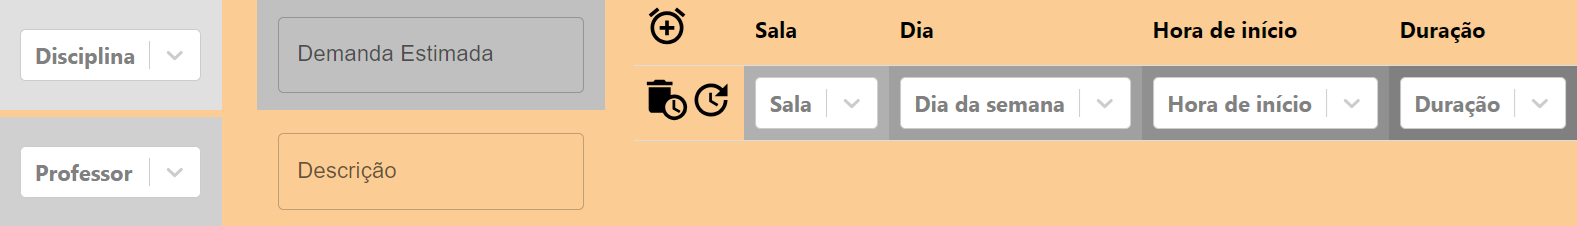
\includegraphics[width=\textwidth]{files/img/2.02!5-desenvolvimento/2.02!5.6-conflitos/Incompletude de informações}
\end{MyCenteredFigure}

A \autoref{fig:turmaVazia} ilustra os \textbf{conflitos nulos}. Esse tipo de conflito representa a incompletude de informações, e como durante parte do processo de criação da grade não se tem todas as informações sobre as alocações das turmas, ele acaba por ser um dos conflitos mais comuns. Esse conflito, representado pela cor acinzentada, é detectado quando um dos campos não se encontra preenchido.

\subsubsection*{\textbf{Conflitos de professores}} \label{sssec:Professores}

O sistema contempla a checagem de conflitos de alocação simultânea de professores em mais de uma turma. Ou seja, considerando todas as turmas às quais o professor está atribuído no ano e semestre selecionados, o sistema compara todos os horários das turmas deste professor, e verifica se há alguma interseção entre horários que estão no mesmo dia, levando em conta a duração da aula.

\begin{MyCenteredFigure} \caption{Exemplo de conflito de alocação de professor} \label{fig:conflitoAlocacaoProfessor}
  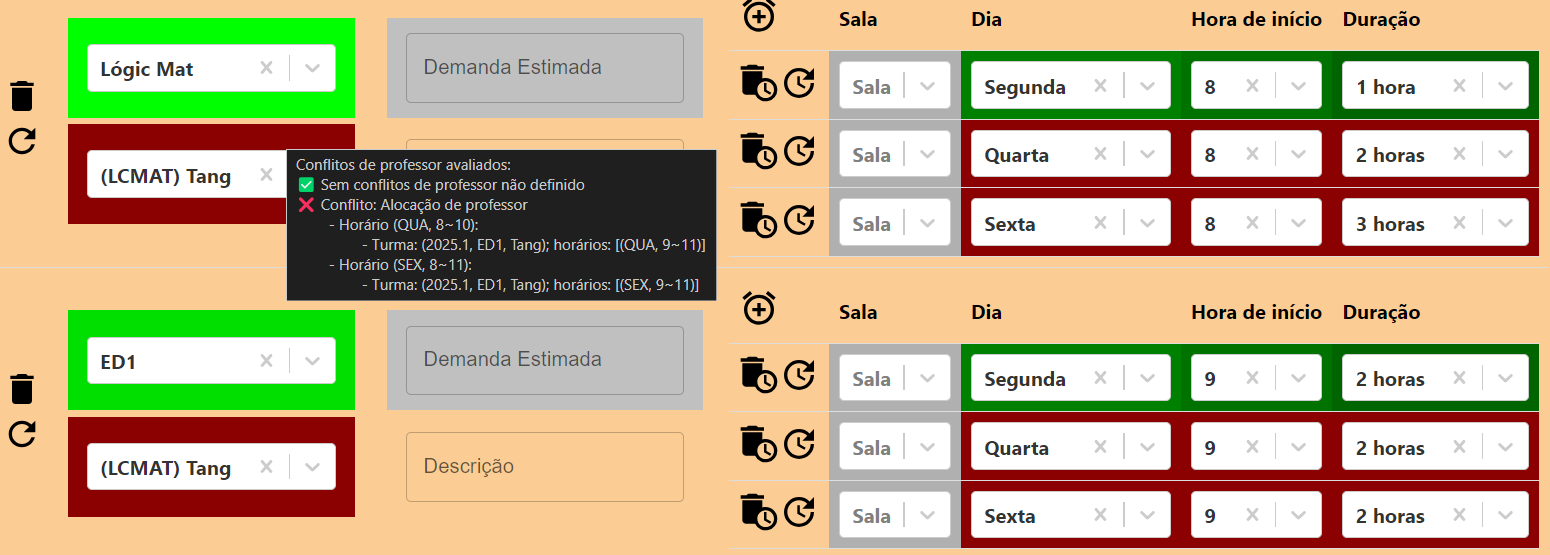
\includegraphics[width=\textwidth]{files/img/2.02!5-desenvolvimento/2.02!5.6-conflitos/Alocação de professores}
\end{MyCenteredFigure}

Caso haja algum conflito, o sistema destaca o professor em questão, tornando a sua cor de fundo avermelhada. Além disso, ao passar o mouse sobre o nome do professor, é exibido um alerta flutuante, informando quais são as turmas e horários que estão em conflito. Esse comportamento é exemplificado na \autoref{fig:conflitoAlocacaoProfessor}, onde o professor Tang é alocado em duas turmas que ocorrem simultaneamente durante algum intervalo de tempo durante os horários de quarta e sexta-feira, assim informando no alerta flutuante quais são as turmas e horários que estão alocados simultaneamente.

\subsubsection*{\textbf{Conflitos de salas}} \label{sssec:Salas}                                 % #### 5.6.1

\begin{MyCenteredFigure} \caption{Exemplo de conflito de alocação de sala} \label{fig:conflitoAlocacaoSalas}
  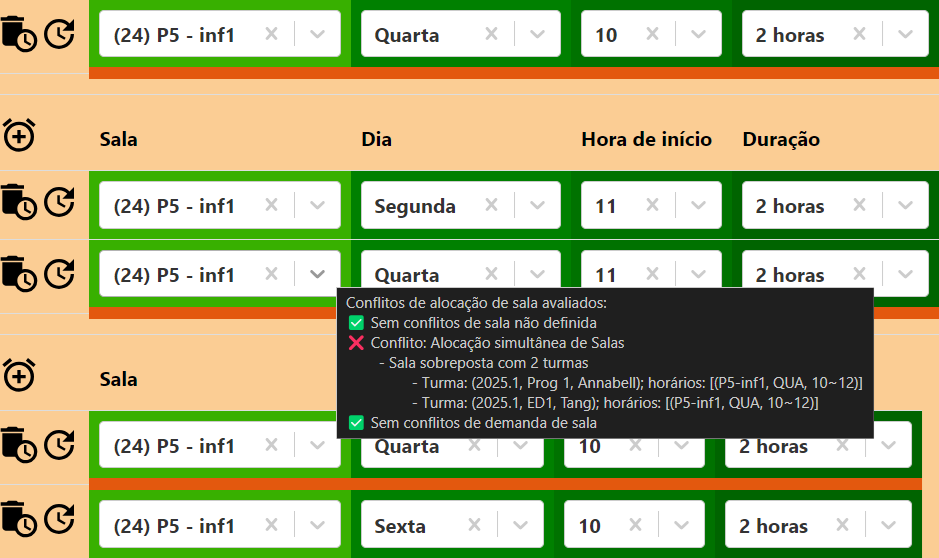
\includegraphics[width=\textwidth]{files/img/2.02!5-desenvolvimento/2.02!5.6-conflitos/Alocação de Salas - Sala}
\end{MyCenteredFigure}

As salas também apresentam a verificação do conflito de alocação simultânea. Porém, diferente dos professores, a checagem é feita conferindo todos os horários na qual a sala está alocada, e então é feita a mesma verificação de interseção citada anteriormente. Havendo o conflito, é exibida uma borda alaranjada na parte inferior das propriedades referentes ao conflito, além de, assim como no caso dos professores, exibir o alerta flutuante. A \autoref{fig:conflitoAlocacaoSalas} representa um caso de conflito de alocação de salas.

\begin{MyCenteredFigure} \caption{Exemplo de conflito de capacidade na sala} \label{fig:conflitoAlocacaoSalasCapacidade}
  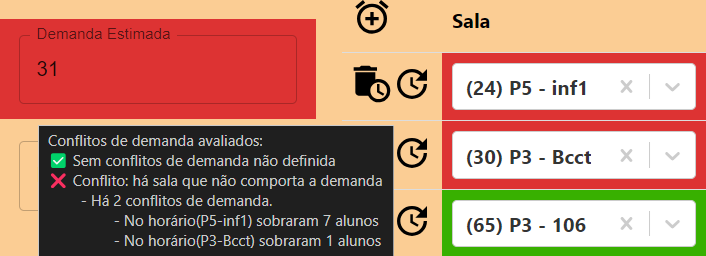
\includegraphics[width=\textwidth]{files/img/2.02!5-desenvolvimento/2.02!5.6-conflitos/Demanda X Capacidade}
\end{MyCenteredFigure}

Além disso, também é feita a comparação entre a quantidade máxima de alunos comportados na sala e a quantidade de alunos estimados para a turma. Este conflito por sua vez é ilustrado tornando avermelhado o fundo da demanda estimada e da seleção de salas. Caso uma turma tenha mais de um horário, é calculada a quantidade remanescente dos alunos que demandam a disciplina com relação a cada uma das capacidades das salas destes horários, mostrando cada um deles no alerta flutuante.

Então, como pode-se perceber na \autoref{fig:conflitoAlocacaoSalasCapacidade}, a turma ilustrada apresenta demanda estimada de 31 alunos não poderia ser adequadamente alocada às salas ``P5 - inf1'', nem na ``P3 - Bcct'', visto que a primeira apenas comporta 24 alunos e a segunda, 30 alunos. O alerta flutuante, ao ser acionado, informa ainda quantos são os alunos que não poderiam ser alocados em cada uma das salas.

\subsubsection*{\textbf{Conflitos de disciplina}} \label{sssec:Disciplina}                       % #### 5.6.2

\begin{MyCenteredFigure} \caption{Avisos flutuantes dos conflitos de disciplinas A} \label{fig:conflitoDisciplinaTitulos_A}
  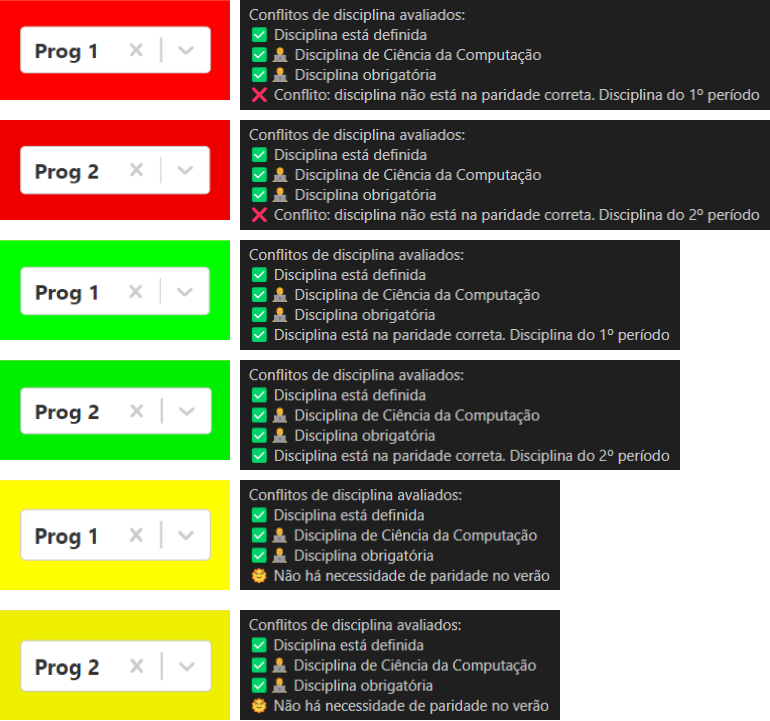
\includegraphics[width=0.8\textwidth]{files/img/2.02!5-desenvolvimento/2.02!5.6-conflitos/Categorias Disciplinas A}
\end{MyCenteredFigure}

Além desses conflitos, outras características analisadas e representadas se referem às disciplinas atribuídas às turmas, que, embora não representem necessariamente um \textit{conflito}, mas sim um indicativo, ainda assim serão tratados como conflitos por motivos de simplificação. Esse indicativo leva em consideração o semestre selecionado e o período esperado da disciplina de certa turma. Utilizando de lógica similar, também é indicado caso não tenha sido atribuído um período à disciplina, e se, para o curso de Ciência da Computação, a disciplina é considerada como \textbf{Eletiva Livre}, \textbf{Eletiva Optativa}, ambas em tons azulados, ou se não é uma disciplina para o curso de Ciência da Computação, sendo então representada em tons alaranjados. Estas características são ilustradas no lado direito da \autoref{fig:conflitoDisciplinaTitulos_A}.

\begin{MyCenteredFigure} \caption{Avisos flutuantes dos conflitos de disciplinas B} \label{fig:conflitoDisciplinaTitulos_B}
  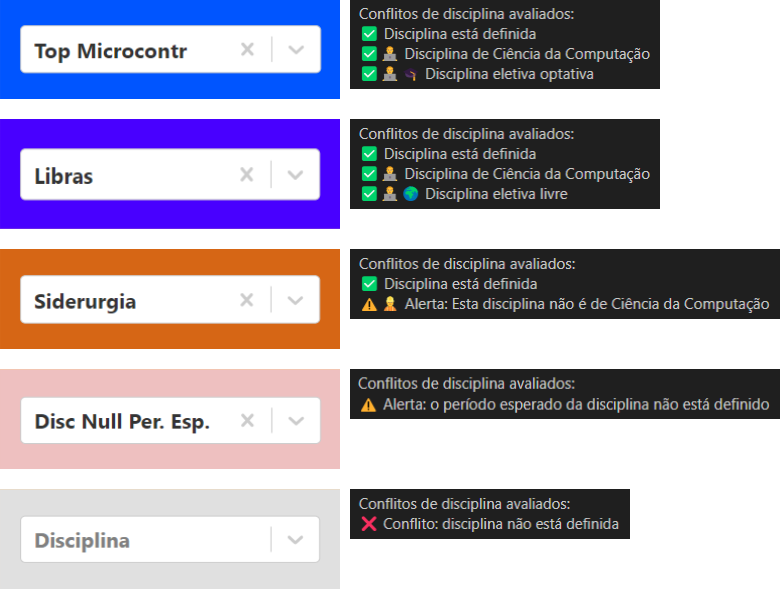
\includegraphics[width=0.8\textwidth]{files/img/2.02!5-desenvolvimento/2.02!5.6-conflitos/Categorias Disciplinas B}
\end{MyCenteredFigure}

Já no lado esquerdo da \autoref{fig:conflitoDisciplinaTitulos_B}, vemos os conflitos que correlacionam os períodos esperados das disciplinas obrigatórias do curso de Ciência da Computação com o semestre em que foram ofertadas. Os semestres possíveis são três: o primeiro semestre, o segundo semestre e o ``período de verão''. No caso do período de verão, as disciplinas que têm o seu período esperado neste semestre são marcadas com um tom amarelado, visto que não há relevância da sua paridade em um período de férias. Já nos casos das disciplinas de paridade ímpar (disciplinas dos períodos 1, 3, 5, 7 e 9) no primeiro semestre, ou as disciplinas de paridade par (disciplinas dos períodos 2, 4, 6, 8 e 10) no segundo semestre, estas são marcadas com um tom esverdeado, sendo aquelas referentes aos períodos finais do curso marcadas com um tom mais escuro. Já as disciplinas pares em semestres ímpares, ou as disciplinas ímpares em semestre pares, são ilustradas com a cor avermelhada, seguindo a mesma lógica de gradiente escuro nos últimos períodos.

\subsection{Resolução dos conflitos} \label{ssec:Resolução}                             % #### 5.6.3

A resolução dos conflitos é feita de forma manual, e o sistema não apresenta uma funcionalidade que permita a resolução automática dos conflitos. A resolução é feita através da análise dos alertas flutuantes e das cores identificadoras dos conflitos, e então, a partir disso, o usuário pode tomar a ação necessária para a resolução dos conflitos. A sequência de ações necessária para a resolução dos conflitos é arbitrária aos gostos do usuário, sendo fortemente dependente da subárea do problema que o usuário deseja resolver. Ainda assim, de forma geral é listado no \autoref{code:pseudo} um pseudo-algoritmo que descreve uma possível sequência para a resolução dos conflitos.

\begin{lstlisting}[language=Python, caption={Pseudo-algoritmo para a resolução de conflitos}, label={code:pseudo}]
def resolveConflitos():
  while ha_informacoes_faltantes():
    adicione_informacoes_faltantes()
    while ha_conflitos():
      ordene_tipos_de_conflitos_por_prioridade()
      for tipo_de_conflito in tipos_de_conflitos:
        conflitos_selecionados = selecione_conflitos(tipo_de_conflito)
        for conflito in conflitos_selecionados:
          analise_grade_horaria_da_entidade_em_questao(conflito)
          realocar_entidade_para_onde_nao_haja_conflito()
\end{lstlisting}

\begin{comment}
Início
Enquanto (a grade estiver incompleta) faça:
Adicione as informações faltantes
Enquanto (houver conflitos) faça:
Ordenar tipos de conflitos por prioridade
Para cada (tipo de conflito) faça:
Selecionar todos os conflitos desse tipo
Para cada (conflito) faça:
Analisar a grade horária da entidade em questão
Alocar a entidade a um novo conjunto de variáveis que não gere conflito
Fim Para
Fim Enquanto
Fim Enquanto
Fim
\end{comment}

\section{Preenchimento de dados} \label{sec:preenchimento}                              % ###  5.7

Inicialmente, os dados adicionados faziam jus diretamente às disciplinas, professores, salas e turmas do curso de Ciência da Computação. Porém, como para a análise completa dos conflitos é necessário que seja feita também a adição das turmas de outros cursos, foi feito o preenchimento de dados para as entidades de professores, disciplinas e salas.

Para acumular mais dados referentes às entidades do banco de dados, foram tomadas algumas abordagens: requisição dos dados diretamente do Sistema Acadêmico, processamento de tabelas, processamento de PDFs e \textit{web scraping}, todos eles ilustrados pela \autoref{fig:DataFlow}.

\begin{MyCenteredFigure} \caption{Diagrama do fluxo de obtenção de dados} \label{fig:DataFlow}
  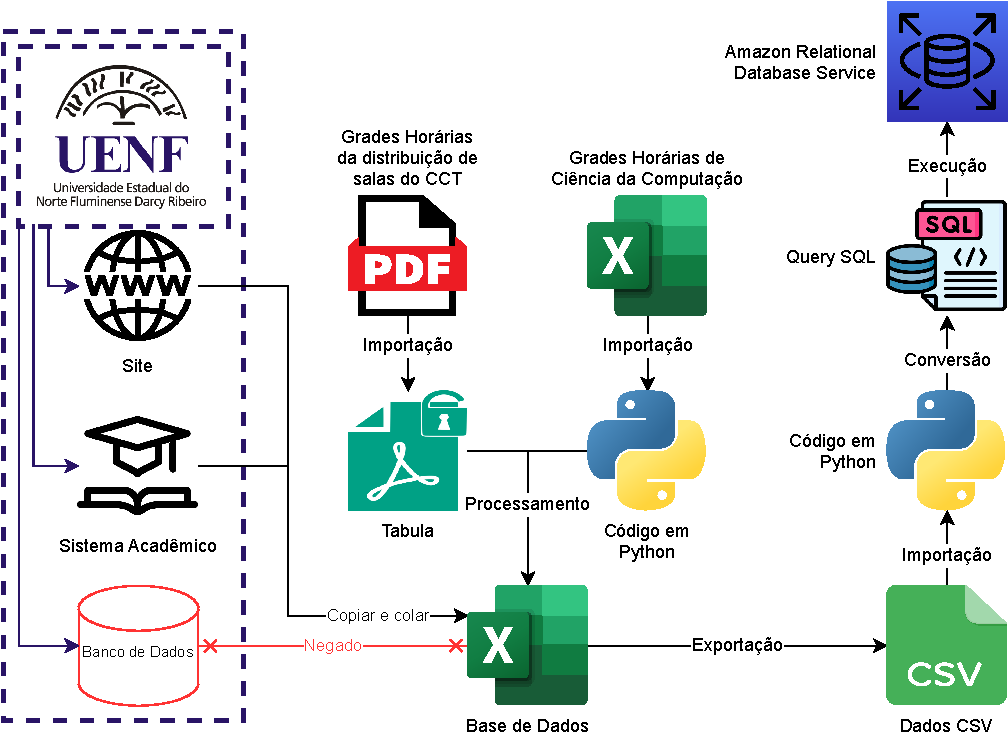
\includegraphics[width=\textwidth]{files/img/2.02!5-desenvolvimento/2.02!5.7-preenchimento/Processamento de dados}
\end{MyCenteredFigure}

A forma teoricamente mais direta e eficiente para se obter os dados das entidades é a obtenção das informações contidas no banco de dados do sistema acadêmico. Para este fim, foi feita uma solicitação ao responsável pela Secretaria Acadêmica (SECACAD) da UENF, que direcionou a solicitação ao desenvolvedor do Sistema Acadêmico. A resposta obtida do desenvolvedor foi que a solicitação não poderia ser atendida, visto que não detinha a posse dos dados, e que para que pudesse fornecê-los, seria necessária uma solicitação formal à reitoria da UENF. Essa solicitação foi então passada à Coordenação do curso de Ciência da Computação, com o qual ficou decidido abandonar a ideia e buscar outras formas de obtenção dos dados.

Paralelamente à abordagem anterior foram feitas tentativas individuais de obtenção dos dados. O processamento de tabelas e PDFs e o \textit{web scraping} foram as abordagens utilizadas. Inicialmente os dados foram coletados e armazenados em tabelas, e então, convertidos para o formato CSV. Os arquivos CSV, por sua vez, foram utilizados em \textit{scripts} Python que os convertiam em \textit{queries} SQL, para que assim então fossem adicionados ao banco de dados.

Os PDFs analisados dispunham de tabelas referentes à oferta de turmas para o CCT, mas os dados advindos do processamento de PDF não são tão estruturados quanto os de uma tabela Excel, por este motivo, a primeira abordagem foi a solicitação dos arquivos tabulares para aquele que os produziu. Não havendo resposta favorável quanto a isso, diversos \textit{softwares} de conversão de tabelas em PDF para Excel foram testados, porém, nenhum deles foi capaz de converter as tabelas de forma satisfatória. Um dos agravantes é a existência de células mescladas, o que torna mais complicada a conversão direta. Outra abordagem testada foi a de importação direta dos PDFs através do Excel e também o simples copiar e colar. Nenhum desses métodos foi eficiente, então com isso alguns dados foram coletados, mas sem certeza quanto à sua precisão. Deste método foram coletadas as informações referentes à nomes de professores e disciplinas, capacidades das salas, e horários de aulas.

Além dos PDFs anteriores, haviam também os arquivos referentes à oferta de turmas para o curso de Ciência da Computação. Estes sim dispunham também de sua versão em Excel, e assim, foram processados utilizando \textit{scripts} Python. A abordagem apresentou falhas, visto que a notação das informações não apresentava o mesmo padrão ao longo dos anos, então foi necessário fazer ajustes manuais, resultando em uma tabela normalizada com diversas pastas de trabalhos referentes a cada um dos semestres desde 2019, não considerando os semestres de verão. Deste método foram coletadas as informações referentes à nomes e apelidos de professores e disciplinas, demandas estimadas dos alunos pela turma, descrição da turma, e horários de aulas.

Por fim, foi feita o \textit{web scraping} que consistiu na busca por informações em diversos sites, principalmente o \LinkToURL{\LinkAcademicoUENF}{Sistema Acadêmico}, o \LinkToURL{\LinkSiteUENF}{site da UENF} e outros sites. Nessa etapa, foi possível encontrar lotes de informações estruturadas. Um dos lotes foi a listagem de disciplinas e suas características que se encontram disponíveis no Sistema Acadêmico da UENF, essas informações foram copiadas e coladas no arquivo Excel unificado. Outros lotes foram encontrados dispersos ao longo do site da UENF e consistiam basicamente em listagem de professores e seus respectivos laboratórios. Essas informações estavam dispersas dos sites dos diversos centros e cursos, alguns disponíveis no próprio site, outros em formato de arquivo. Deste método foram coletadas as informações referentes à nomes de professores, seus laboratórios e centros; e disciplinas e seus nomes, códigos e períodos de vigência. Além disso, foram encontrados documentos oficiais que referenciam a capacidade de ocupantes das ``salas'' disponíveis do Centro de Convenções, popularmente conhecido como ``Apitão'' que mesmo não sendo propriamente uma sala de aula, já foi utilizado previamente para tal fim. Outras salas já obtiveram alocações similares, assim como a Sala dos Professores.

\section{Próximos desenvolvimentos} \label{sec:proximos}                                % ###  5.8

Ao longo de todo o desenvolvimento, podemos dividir as funcionalidades em quatro categorias: as que foram \textbf{implementadas e se mantiveram}, as que foram \textbf{implementadas e descartadas}, as que \textbf{não foram implementadas} e as que foram \textbf{preparadas} para próximos desenvolvimentos.

As \textbf{implementadas e se mantiveram} são aquelas principais e essenciais para o funcionamento do sistema, como a adição de turmas, professores, disciplinas e salas, a visualização da grade horária, a detecção de conflitos.

As \textbf{implementadas e descartadas} são aquelas que por diversos motivos, não se mantiveram no sistema. Um exemplo disso é a funcionalidade de travamento de turmas, que foi implementada, mas descartada por não ser considerada essencial.

As \textbf{não implementadas} são aquelas que, devido a priorização das tarefas, não detiveram importância o bastante para que chegassem à etapa de implementação. Um exemplo disso é a funcionalidade de alterar a grade horária através do sistema de arrastar e soltar.

As \textbf{preparadas mas não implementadas} são aquelas que, por conveniência ou por praticidade do momento, foram parcialmente desenvolvidas, mesmo que não tenham grande participação no sistema final. Dentre elas, podemos citar a funcionalidade de adição de alunos, e diversas tabelas e colunas no banco de dados que foram criadas e preenchidas mas não utilizadas.

\subsection{Funcionalidades preparadas} \label{ssec:Funcionalidades preparadas}         % ###  5.8.1

Dentre as funcionalidades preparadas temos o sistema de cadastro de alunos, que consiste basicamente na adição das informações básicas dos alunos, como ano de entrada, curso, matrícula e nome como é visto em sua tabela no canto inferior direito na \autoref{fig:DER final}. Seus dados podem ser armazenados no banco de dados junto com os outros dados das entidades que são mais diretamente relacionadas à grade horária, como as turmas, professores, disciplinas e salas.

Além dos alunos, outras entidades também foram estruturadas, sendo elas os centros e laboratórios. Isso se deu com o objetivo de estruturar mais objetivamente as informações referentes aos professores e disciplinas, visto que os professores são vinculados a um centro e a um laboratório, assim tendo a tendência a reduzir a necessidade de repetição de informações.

\begin{MyCenteredFigure} \caption{Diagrama entidade relacionamento final} \label{fig:DER final}
  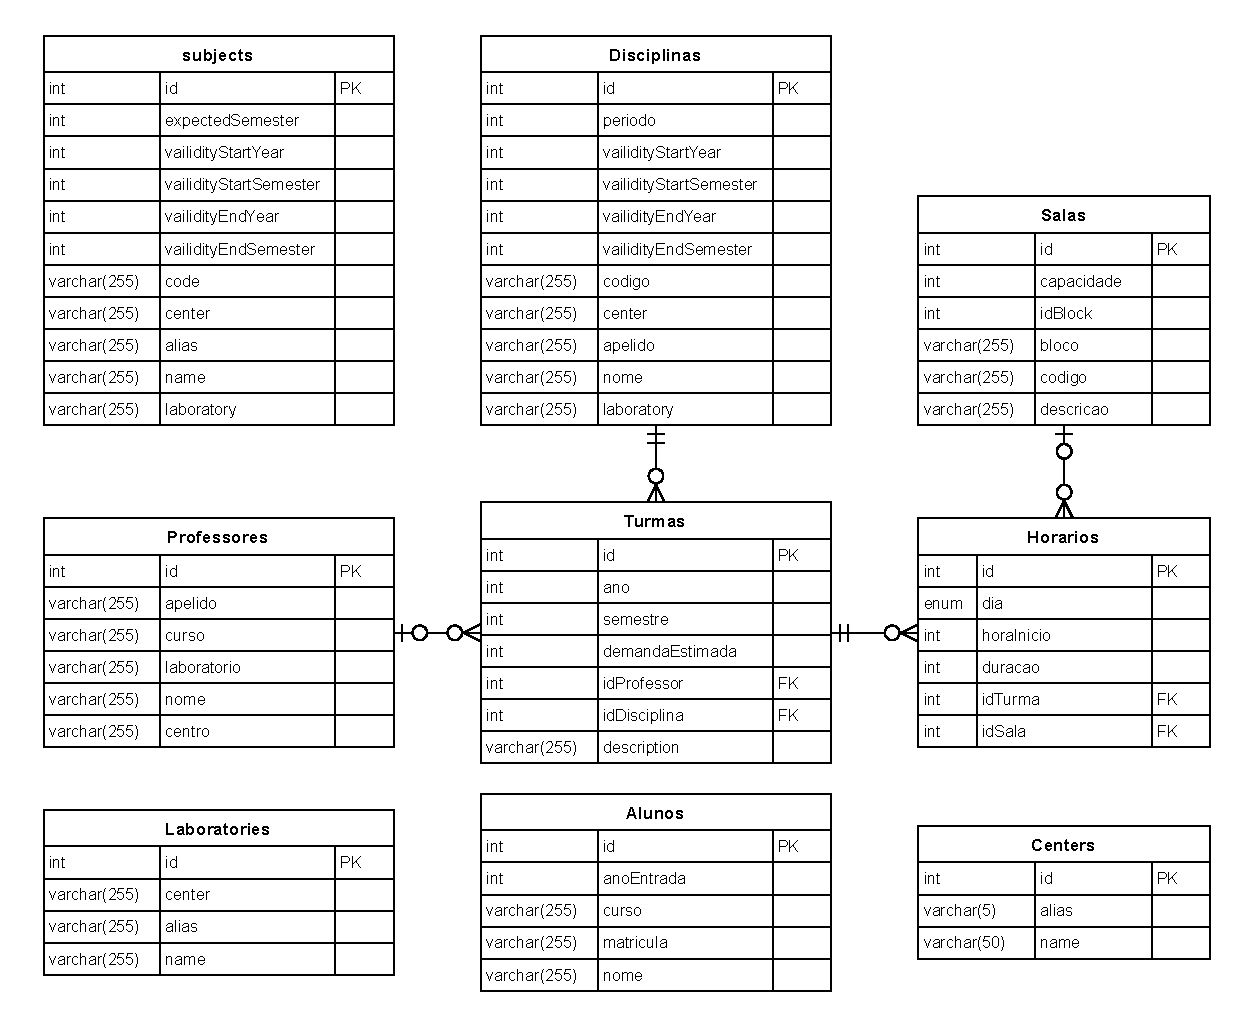
\includegraphics[width=\textwidth]{files/img/2.02!5-desenvolvimento/2.02!5.8-proximos/Diagrama ER-Final}
\end{MyCenteredFigure}

Nota-se que na \autoref{fig:DER final}, alguns atributos encontram-se em inglês e outros em português. Isso se dá pelo fato de que a transição para o inglês foi feita de forma gradual, e embora a maior parte do sistema já esteja em inglês, ainda há partes que se encontram em português. A decisão pela migração para o inglês se deu pelo fato de que na programação de modo geral, as variáveis e funções são escritas em inglês, e embora não seja uma regra, torna o código mais consistente em sua linguagem.

A interface para definição da preferência dos professores também se encontra pronta, e consiste em uma tabela onde cada linha representa um horário e cada coluna representa um dia da semana. Nela, o professor pode marcar os horários em que não pode ministrar aulas, e também indicar os horários em que prefere ministrar aulas. Essa funcionalidade pode vir a ser retomada posteriormente por auxiliar na tomada de decisão voltada a alocação dos professores bolsistas, visto que geralmente são os que menor se sabe sobre a disponibilidade, então, tendo a possibilidade de marcar os horários em que não podem ministrar aulas, pode-se evitar a alocação de turmas nesses horários.

Outro sistema também preparado envolve a visualização da progressão de disciplinas dos alunos que foi dividida basicamente em três categorias: \textbf{aprovadas}, \textbf{cursando} e \textbf{reprovadas}. A visualização era feita em uma caixa de seleção de múltipla escolha, onde as opções eram todas as disciplinas disponíveis. Com esse registro, torna-se possível ter uma estimativa calculada da demanda de alunos para as turmas, pois considera-se a quantidade de alunos que ainda não a concluíram, seja por reprovação ou por escolherem não se inscrever. Tendo também o histórico de reprovações médias, pode-se calcular mais precisamente a demanda de alunos para as turmas. Cada uma dessas funcionalidades foi parcialmente implementada, podendo ser então retomadas e finalizadas em futuros desenvolvimentos.
